\documentclass[a4paper,12pt,twoside,final]{book}

\usepackage[utf8]{inputenc}

\usepackage[spanish,es-nodecimaldot]{babel} % International, rec. by RAE: http://www.tex-tipografia.com/marca_decimal.html
%\usepackage[backend=bibtex, maxbibnames=99, giveninits=true]{biblatex}
\usepackage[backend=biber, maxbibnames=99, giveninits=true]{biblatex}

\addbibresource{references.bib}
% COLOR
\usepackage[usenames,dvipsnames,svgnames,table]{xcolor}



% Colores para estilo Proyecto Docente (tonos naranjas)
\definecolor{lightback}{HTML}{F4E0BF}
     \definecolor{back}{HTML}{F3C591}
\definecolor{lightline}{HTML}{FCAF5F}
     \definecolor{line}{HTML}{ED7900}
% Colores para portada
\definecolor{epsc:oscuro}{HTML}{280091}
 \definecolor{epsc:medio}{HTML}{4C5CC5}
 \definecolor{epsc:claro}{HTML}{3FCFD5}
 \definecolor{epsc:verde}{HTML}{00B299}


\usepackage{float}
\usepackage{lscape}

\usepackage{tikz} % used in cover to place images

\usepackage{datetime} % allow formal date format
% "Month, YEAR" date format, in spanish with the month uppercased not interfering other dates
\newcommand\Monthname[1][EMPTY]{
  \ifnum1=#1Enero\else
  \ifnum2=#1Febrero\else
  \ifnum3=#1Marzo\else
  \ifnum4=#1Abril\else
  \ifnum5=#1Mayo\else
  \ifnum6=#1Junio\else
  \ifnum7=#1Julio\else
  \ifnum8=#1Agosto\else
  \ifnum9=#1Septiembre\else
  \ifnum10=#1Octubre\else
  \ifnum11=#1Noviembre\else
  \ifnum12=#1Diciembre\else
  \fi\fi\fi\fi\fi\fi\fi\fi\fi\fi\fi\fi
}
\newdateformat{monthyeardate}{%
  \Monthname[\THEMONTH], \THEYEAR}


% FONTs
\usepackage[T1]{fontenc}
\usepackage{textcomp}           % Needed for new symbols like € ?

\usepackage[scaled]{berasans} % Font for the cover similar to Vera 33
%\renewcommand*\familydefault{\sfdefault}  %% To use as the base font of the document is to be sans serif


% PAGE STYLE
\usepackage[twoside,bindingoffset=0cm,headheight=30pt,margin=25mm]{geometry} %,verbose,showframe
\usepackage{fancyhdr} % Encabezados
\pagestyle{fancy}
\fancyhf{}
\fancyhead[LE]{\leftmark}
\fancyhead[RO]{\rightmark}
\fancyfoot[RO,LE]{\thepage}
% XXX Evitar el binding en la portada pero no en el resto del documento

% Sangría para párrafo, tabulaciones de 1 cm
\parindent=1.0cm
% Espacio o separación entre párrafos
\parskip 1.5ex

% TABLES AND FIGURES
\usepackage{graphicx}
\graphicspath{ {img/} }

\usepackage{todonotes}
\usepackage{float}
\usepackage{tabularx}
\usepackage{url}
\usepackage{emptypage}
\usepackage[toc,page]{appendix}
\usepackage{hyperref}
\hypersetup{ colorlinks=true,                     %habilitar colorear enlaces
            linkcolor=black,
            filecolor=black,
            urlcolor=cyan,
            citecolor=blue,
            }
\usepackage{array}
\usepackage{wrapfig}
\usepackage{multirow}
\usepackage{multicol} %Para poner columnas de un solo elemento
\usepackage{tabu}

\usepackage{pifont} %Para usar el vmark (tick) y xmark (cross)
\newcommand{\vmark}{\textcolor{green}{\ding{51}}} %Definición del vmark en verde
\newcommand{\xmark}{\textcolor{red}{\ding{55}}} %Definición del xmark en rojo

\usepackage{chngcntr}
\usepackage{verbatim}
\usepackage{graphicx}
\usepackage[export]{adjustbox}
\usepackage{listings}
%\usepackage{minted}

\usepackage{booktabs,caption}
\usepackage[flushleft]{threeparttable}
\usepackage{fancyvrb}
\usepackage{verbatimbox}
\usepackage{afterpage}

\usepackage{csquotes}

\usepackage{rotating} % para rotar tablas

\newsavebox{\FVerbBox}
\newenvironment{FVerbatim}
 {\VerbatimEnvironment
  \begin{center}
  \begin{lrbox}{\FVerbBox}
  \begin{BVerbatim}}
 {\end{BVerbatim}
  \end{lrbox}
  \fbox{\usebox{\FVerbBox}}
  \end{center}}
  
  
  \newcommand\blankpage{%
    \null
    \thispagestyle{empty}%
    \addtocounter{page}{-1}%
    \newpage}
    
\counterwithout{footnote}{chapter}
  
\begin{document}
\frontmatter

%------------- Cover --------------
\thispagestyle{empty}

% Backgroud images
\begin{tikzpicture}[remember picture, overlay]
  % Top
  \node [anchor=north east, inner sep=0pt]  at (current page.north east)
     {
\includegraphics[height=6cm]{topRightCorner.pdf}};
  % Bottom
  \node [anchor=south west, inner sep=0pt]  at (current page.south west)
     {
\includegraphics[height=6cm]{bottomLeftCorner.pdf}};
  \node (uco) [anchor=south east, inner sep=0pt, xshift=-10mm, yshift=10mm]  at (current page.south east)
        {
\includegraphics[height=2cm]{uco_debajo.pdf}};
  \node [anchor=south east, inner sep=0pt, xshift=-10mm]  at (uco.south west)
% Uncomment the chosen logo and comment the others:
        {
\includegraphics[height=2cm]{emblema-ing-informatica.pdf}};
%        {
\includegraphics[height=2cm]{emblema-ing-industrial.pdf}};
%        {
\includegraphics[height=2cm]{emblema-ing-tec-industrial.pdf}};
\end{tikzpicture}

\renewcommand*\listtablename{Índice de tablas}
\renewcommand{\tablename}{Tabla}
\begin{center}
\fontfamily{\sfdefault}\selectfont
\vspace*{2cm}

\vfill
\vfill

\includegraphics[width=12.5cm]{LogotipoEPSC.pdf}
\vfill
\vfill

\large\textbf{\color{epsc:medio}
  TRABAJO FIN DE GRADO
}
\vfill

\Large\textbf{\color{epsc:verde}
  Grado en Ingeniería Informática
}
\vfill
\large\textbf{\color{epsc:verde}
 Especialidad de Ingeniería del Software
}
\vfill

\Huge\textbf{\color{epsc:oscuro}
  Aplicación web para la gestión de comisiones de los centros pertenecientes a la Universidad de Córdoba
  }
\vfill
\vfill
\Large\textbf{\color{epsc:verde}
  Manual Técnico
}
\vfill
\vfill

\large{\color{epsc:oscuro}Autor}\\
\textbf{\color{epsc:medio}{ Javier Ruiz Jurado }}
\vfill

\large{\color{epsc:oscuro} Director }\\
\textbf{\color{epsc:medio} José Luis Ávila Jiménez }
\vfill

\textbf{\color{epsc:verde} \monthyeardate\today}
\vfill
\vfill
\vspace{2.7cm}
\end{center}

%-------------------------------------------------------------------------------------------------------
\clearpage

\thispagestyle{empty}
\pagecolor{white}

\cleardoublepage
%-------------------------------------------------------------------------------------------------------
\cleardoublepage

\thispagestyle{empty}
\pagecolor{white}

\Large{\textbf{
    Agradecimientos }}

\normalsize{}

Agradecer a mi familia su apoyo y comprensión. Quiero hacer una mención especial a todos aquellos profesores que durante mi carrera académica me han ayudado, enseñado sus conocimientos y experiencias.

A todos ellos muchas gracias.

\cleardoublepage
%-------------------------------------------------------------------------------------------------------  

\cleardoublepage
\setcounter{page}{1}
\setcounter{tocdepth}{3} %Numeración anidada de profundidad 3 en el índice
\setcounter{secnumdepth}{3} %Numeración anidada de profundidad 3 en los capítulos
\tableofcontents
\listoffigures
\listoftables
%\cleardoublepage

\afterpage{\null\newpage}
\thispagestyle{empty}
\newpage
\mainmatter

%Insertar capítulos
\part{Presentación}
\chapter{Introducción}

\section{Comisiones de centros de la Universidad de Córdoba}

La Universidad de Córdoba (UCO)\cite{uco} es una institución universitaria localizada en la ciudad de Córdoba y fundada en el año 1972. La UCO cuenta actualmente con un total de diez centros propios, dos centros adscritos, el Instituto de Estudios de Posgrado (IDEP) y el Centro Intergeneracional ``Francisco Santisteban''. Los centros propios están organizados en cuatro Campus universitarios: tres en la ciudad y uno en Belmez.
   \begin{itemize}
    \item \textbf{Centros propios}
        \begin{itemize}
        \item Facultades:
            \begin{itemize}
                \item Facultad de Ciencias (Campus de Rabanales).
                \item Facultad de Ciencias de la Educación y Psicología (Campus de Menéndez Pidal).
                \item Facultad de Ciencias del Trabajo  (Campus del Centro Histórico).
                \item Facultad de Derecho y Ciencias Económicas y Empresariales (Campus del Centro Histórico).
                \item Facultad de Filosofía y Letras (Campus del Centro Histórico).
                \item Facultad de Medicina y Enfermería  (Campus de Menéndez Pidal).
                \item Facultad de Veterinaria (Campus de Rabanales).
            \end{itemize}
        \item Escuelas:
        \begin{itemize}
            \item Escuela Politécnica Superior de Belmez (Campus de Belmez).
            \item Escuela Politécnica Superior de Córdoba (Campus de Rabanales).
            \item Escuela Técnica Superior de Ingeniería Agronómica y de Montes (Campus de Rabanales).
        \end{itemize}
    \end{itemize}
    \item \textbf{Centros adscritos}
    \begin{itemize}
        \item Centro de Magisterio ``Sagrado Corazón'', con sede en Córdoba.
        \item Centro Universitario FIDISEC, con sede en Cabra.
    \end{itemize}
\end{itemize}    

Cada uno de estos centros, ya sea facultad o escuela, actúan para el cumplimiento de sus fines a través de los siguientes órganos de gobierno y representación, formando el \textbf{Equipo de Gobierno} del centro \cite{reglamento}: 
\begin{itemize}
    \item \textbf{Junta de Centro o Escuela}: es el órgano colegiado de gobierno, que ejerce sus funciones con sujeción a los acuerdos del Equipo de Gobierno y a las resoluciones del Rector, de acuerdo con lo establecido en los Estatutos de la Universidad de Córdoba y en el actual Reglamento. Entre sus funciones principales, se encarga de tomar las decisiones y establecer las políticas académicas y administrativas del centro.
    \item \textbf{Decano o Director}: ostenta la representación de la Facultad o Escuela, respectivamente, y ejerce las funciones de dirección y gestión ordinaria de la misma. 
    \item \textbf{Vicedecanos o Subdirectores}: el Decano o Director podrá proponer, para su nombramiento por el Rector, a Vicedecanos o Subdirectores, respectivamente, entre los profesores con vinculación permanente a la universidad adscritos al Centro, en los que podrá delegar funciones que le son propias

    \item \textbf{Secretario}: será nombrado por el Rector, a propuesta del Decano o Director, entre los profesores con vinculación permanente a la Universidad de Córdoba adscritos al Centro, en los que podrá delegar funciones que le son propias.

\end{itemize}

La Junta de Centro o Escuela podrá crear cuantas Comisiones considere necesarias para el buen desarrollo de sus funciones. Las \textbf{Comisiones} son grupos de trabajo especializados que se crean dentro del centro para abordar temas específicos, como la planificación curricular, la investigación o la gestión de recursos. Los miembros de estas Comisiones serán elegidos o designados por la Junta de Centro o Escuela entre personal docente e investigador, personal de administración y servicios y estudiantes, atendiendo a la naturaleza de la Comisión.

Existirán al menos las siguientes Comisiones en cada centro:
\begin{itemize}
    \item Comisión de Asuntos Económicos.
    \item Comisión de Docencia.
    \item Comisión de Ordenación Académica.
    \item Comisión de Relaciones Exteriores.
    \item Comisión de Reconocimientos y Convalidaciones.
    \item Comisión Académica de los Másteres.
    \item Unidades de Garantía de Calidad.
\end{itemize}
    
\section{Definición del problema real}
    
    Existe un problema generalizado con respecto a la gestión de las comisiones de los distintos centros pertenecientes a la Universidad de Córdoba, el cual viene dado principalmente por la ausencia de un sistema informático de gestión.
    
    Actualmente, se realizan tareas manuales y estáticas sobre estas comisiones que provocan que la gestión administrativa sobre ellas sea una tarea lenta de realizar, sin conseguir una trazabilidad de los movimientos de altas/bajas de sus miembros, pérdida de tiempo con respecto a utilizar un sistema que automatice lo máximo posible alguna de sus gestiones...

    En resumen, el problema real que se desea resolver con el desarrollo de este Trabajo de Fin de Grado es el siguiente: los centros (facultades y escuelas) de la Universidad de Córdoba no poseen una aplicación informática que permita la gestión de sus comisiones universitarias.
    
 
\section{Definición del problema técnico}

    Se va a utilizar la metodología denominada \textit{Product Design Specification} (PDS) para describir el problema técnico que se desea resolver. Esta metodología permite dar respuesta a una serie de apartados que se enumeran a continuación.
    
\subsection{Funcionamiento}
    Se desea implementar una aplicación web que permita realizar una gestión de las comisiones pertenecientes a los centros de la Universidad de Córdoba. 
    
    Los usuarios que interactuarán con la aplicación son los siguientes:
    \begin{itemize}
        \item Administrador
          \begin{itemize}
              \item Este tipo de usuario estará registrado en el sistema y tendrá un control completo de la aplicación. 
              \item En particular, tendrá las competencias exclusivas de la gestión de todos los tipos de usuarios, centros, juntas, miembros y comisiones. Además, se encargará de la gestión de las copias de seguridad.
          \end{itemize}
          \item Responsable del centro
           \begin{itemize}
               \item Este tipo de usuario estará registrado en el sistema y representará a una persona que podrá gestionar la información de un centro.
               \item En particular, tendrá las competencias exclusivas de la asignación/exclusión a los miembros de gobierno pertenecientes a dicho centro, de creación de las juntas que pertenezcan al centro, así como asignación/exclusión del responsable de cada junta.
            \end{itemize}
            \item Responsable de la junta
           \begin{itemize}
               \item Este tipo de usuario estará registrado en el sistema y representará a una persona que podrá gestionar la información de una junta de centro.
               \item En particular, tendrá las competencias exclusivas de la asignación/exclusión a los miembros de junta pertenecientes a dicha junta, de la gestión de las convocatorias realizadas por la junta, de los miembros que participarán en cada una de las convocatorias de la junta, de creación de las comisiones que pertenezcan a la junta, así como asignación/exclusión del responsable de cada comisión.
            \end{itemize}
          \item Responsable de la comisión 
           \begin{itemize}
               \item Este tipo de usuario estará registrado en el sistema y representará a una persona que podrá gestionar la información de una comisión.
               \item En particular, tendrá las competencias exclusivas de la asignación/exclusión a los miembros pertenecientes a dicha comisión, gestión de las convocatorias realizadas por la comisión, y de los miembros que participarán en cada una de las convocatorias de dicha comisión.
            \end{itemize}
        \item Usuario universitario
            \begin{itemize}
                \item Este tipo de usuario estará registrado en el sistema.
                \item Podrá obtener distintos certificados como pueden ser de situación actual, de centros en los que ha participado como miembro de equipo de gobierno, de juntas a las que ha representado, de comisiones a las que ha pertenecido, de convocatorias en las que ha participado...
              \end{itemize}
        \item Público
        \begin{itemize}
              \item Este tipo de usuario no necesitará estar registrado en el sistema.
              \item Podrá consultar la información pública disponible: comisiones de un centro, miembros actuales de una comisión, consulta de actas aprobadas y pendientes de aprobación,...
          \end{itemize}
     \end{itemize}
     
\subsection{Entorno}
 Existirán dos entornos de trabajo para esta aplicación. 

  \begin{itemize}
     \item Entorno de desarrollo y testeo: entorno que se utilizará para desarrollar, probar y depurar la aplicación web antes de su lanzamiento al entorno de producción.
     \item Entorno de producción:
         entorno en el que se encontrará la versión final de la aplicación web, una vez de pasadas todas las pruebas y correcciones necesarias en el entorno de desarrollo y pruebas. Estará configurado y optimizado para garantizar un rendimiento y disponibilidad óptimos, así como protegido por diferentes medidas de seguridad.
 \end{itemize}

Existirán dos entornos de ejecución para esta aplicación. 

 \begin{itemize}
     \item Entorno de ejecución del administrador:
         el administrador ejecutará la aplicación desde un servidor que le permitirá acceder a todos los recursos de software y así poder modificar cualquier aspecto del sistema.
     \item Entorno de ejecución de los demás usuarios:
         el resto de usuarios (público, registrado, responsable del centro,junta y comisión y miembro de gobierno, junta y comisión) ejecutarán la aplicación desde su propios equipos, siempre que estos tengan conexión a internet al tratarse de una aplicación web.
 \end{itemize}

 La interfaz es el medio de comunicación entre los usuarios y la aplicación web. Es importante que la interfaz sea lo más intuitiva y amigable posible para poder generar una mejor experiencia en el usuario. Los requisitos de la interfaz se describirán en la Sección \ref{sec:requisitos-interfaz}.

 La aplicación web será completamente responsiva, adaptándose a a diferentes tamaños y resoluciones de pantalla de diferentes dispositivos, como móviles, tabletas, ordenadores de escritorio,...

En resumen, una aplicación web responsiva nos brindará una experiencia de usuario cómoda y consistente en todos los dispositivos, mejorando la accesibilidad de la aplicación así como su visibilidad en línea.

        
\subsection{Vida esperada}
    
    El ciclo de vida esperado para dicha aplicación web será alto ya que se considera que prácticamente no van a cambiar las tareas comunes de la gestión de comisiones.
    
    Sin embargo, sí es posible que haya que actualizar la aplicación web debido a la aparición de nuevos recursos de software o hardware, o versiones mejoradas de los mismos, que puedan mejorar la aplicación web que se desea desarrollar: rendimiento, seguridad, etc.
    
\subsection{Ciclo de mantenimiento} \label{subsec:ciclo_mantenimiento}

 Teniendo en cuenta que el propósito de la creación de esta aplicación web es la realización de un Trabajo de Fin de Grado, el mantenimiento de dicha aplicación no correrá a cargo de su autor.

 No obstante, se realizará un diseño modular de cada una de las partes de la aplicación web para facilitar, en el futuro, posibles tareas de mantenimiento y mejoras.


\subsection{Competencia}

 No procede realizar un posible análisis de competencia comercial puesto que se trata del desarrollo de una aplicación web con fines educativos, teniendo como objetivo final el desarrollo de un Trabajo de Fin de Grado.

 Además, no se tiene conocimiento de que la Universidad de Córdoba disponga de una aplicación web para la gestión de las comisiones de sus centros universitarios. Tampoco se conoce la existencia de aplicaciones similares en otras universidades.


\subsection{Aspecto externo}

En relación con el aspecto externo, se tendrán en cuenta los siguientes aspectos:

\begin{itemize}
    \item \textbf{Interfaz de usuario}
    \begin{itemize}
        \item Se realizará una interfaz totalmente responsiva, intuitiva y amigable para que el usuario pueda navegar de la manera más cómoda posible. El Capítulo \ref{cap:diseño_interfaz} describirá el Diseño de la Interfaz de la aplicación web que se va  a desarrollar.
    \end{itemize}
    \item \textbf{Distribución de la aplicación: formato de almacenamiento}
     \begin{itemize}
         \item La aplicación se podrá distribuir a través de un repositorio en la nube.
     \end{itemize}
     
    \item \textbf{Documentación}
     \begin{itemize}
         \item Se elaborarán los siguientes manuales:
        \begin{itemize}
        \item Manual técnico: este documento en el que describirán todas las fases de desarrollo de la aplicación web.
        \item Manual del usuario: describirá la instalación y desinstalación de la aplicación web y las indicaciones para su utilización por los diferentes tipos de usuarios
        \item Manual de código: constará de dos partes. La documentación externa describirá los recursos de hardware y software utilizados, y agrupará el código en bloques funcionales (interfaz, base de datos, etc.). La documentación interna comentará los ficheros de código.
    \end{itemize}
     \end{itemize}
\end{itemize}


\subsection{Estandarización}

 Para el desarrollo de la aplicación web, se revisarán las 
 las recomendaciones propuestas por \textit{World Wide Web Consortium} (W3C) \cite{w3c}, que ``promueve el uso de estándares para reducir el coste y la complejidad del desarrollo, así como para incrementar la accesibilidad y usabilidad de cualquier documento publicado en la web'' \cite{revistadigital}.

 También se debe tener en cuenta que los recursos  que se van a utilizar son herramientas informáticas que están validadas por prestigiosas organizaciones que indican que cumplen con los estándares. Véase el capítulo \ref{cap:recursos} de Recursos. 

\subsection{Calidad y fiabilidad}

 La calidad y la fiabilidad de la aplicación web estará garantizadas por las siguientes razones.
 \begin{itemize}
     \item Se va a utilizar una metodología de Ingeniería del Software para especificar los requisitos (funcionales, no funcionales, de información y de la interfaz), modelar la información que se va a utilizar, analizar las funciones que se van a desarrollar, diseñar el modelo de datos, clases y paquetes, diseñar la interfaz, etc. 
     \item Se van a utilizar recursos de software ampliamente usados y contrastados en el desarrollo de aplicaciones web.
     \item La aplicación web será sometida a un completo proceso de pruebas para comprobar que es correcta, robusta y amigable.
 \end{itemize}

\subsection{Programa de tareas}

 El desarrollo del presente Trabajo de Fin de Grado va estar compuesto por la siguientes fases:
 \begin{itemize}
     \item Introducción: descripción del problema, establecimiento de los objetivos, revisión de antecedentes, identificación de restricciones iniciales y estratégicas y selección de recursos.
     \item Análisis: especificación de requisitos (funcionales, no funcionales, de información y de la interfaz), descripción del modelo de datos y análisis funcional (casos de uso y diagramas de secuencia).
    
     \item Diseño: descripción del diseño de datos, clases, paquetes y de la interfaz.
    
     \item Implementación: codificación de la aplicación web teniendo en cuenta el diseño desarrollado.
    
     \item Pruebas: comprobación de que la aplicación web funciona correctamente, es robusta y amigable.
    
     \item Documentación: redacción del manual técnico (este documento), el manual de usuario y el manual de código.
 \end{itemize}


\subsection{Pruebas}

La fase de pruebas es esencial para garantizar que la aplicación web funciona correctamente. En particular, se pretende comprobar que la aplicación web:
\begin{itemize}
    \item Hace lo que debe hacer.
    \item No provoca efectos secundarios que pueden desencadenar situaciones catastróficas.
    \item Contiene módulos que se ejecutan correctamente.
    \item Garantiza los privilegios de cada tipo de usuario.
\end{itemize}

Cada prueba tendrá la siguiente estructura para detectar los errores y corregirlos:
\begin{itemize}
    \item Objetivo de la prueba. Se debe indicar en qué consiste la prueba y el resultado esperado.
    \item Problema detectado, en su caso. Si ocurre un error entonces se debe describir la causa que lo ha provocado.
    \item Solución adoptada, en su caso. Si se ha producido un error, se deben indicar las medidas tomadas para solucionarlo.
\end{itemize}

El Capítulo \ref{cap:pruebas} de Pruebas describirá las pruebas realizadas.

\subsection{Seguridad}

Hay varias consideraciones de seguridad que se deben tener en cuenta al desarrollar una aplicación web moderna. Algunas de las más importantes son:

\begin{itemize}
    \item Autenticación y autorización: es importante garantizar que los usuarios sean autenticados correctamente antes de permitirles el acceso a diferentes vistas de la aplicación. Además, es necesario asegurarse de que los usuarios solamente tengan los permisos necesarios para realizar acciones específicas dependiendo del tipo de usuario autenticado. Además, se utilizará el control de sesiones para garantizar que un usuario no puede acceder directamente a una página web de la aplicación tecleando su dirección url si antes no se ha identificado con su clave y contraseña.

    \item Protección contra ataques de inyección: Las aplicaciones web modernas pueden ser vulnerables a ataques de inyección, como inyección de SQL o inyección de código. Es importante utilizar técnicas de validación y filtrado de datos para proteger la aplicación de estos ataques.

    \item Protección de datos: para garantizar la confidencialidad de información que establece la Ley Orgánica de Protección de Datos (LOPD) \cite{lopd}, es importante asegurarse de que los datos sensibles estén cifrados y de que la aplicación esté protegida contra la exposición de datos confidenciales.
\end{itemize}



\chapter{Objetivos}
\section{Objetivo principal}
 El objetivo de este Trabajo de Fin de Grado es el desarrollo de una aplicación web para la gestión de las comisiones de los centros de la Universidad de Córdoba: facultades y escuelas superiores. En particular, se desea gestionar la información de sus juntas de centro o juntas de escuela y de las comisiones delegadas de las mismas, como las comisiones de docencia, planes de estudios, asuntos económicos, etc.

\section{Objetivos específicos}

Los objetivos específicos de este Trabajo de Fin de Grado son los siguientes:

\begin{itemize}
    \item \textbf{Tipos de usuarios}
    \item[] Se deberán permitir los siguientes tipos de usuarios: 
     \begin{itemize}
        \item Administrador
          \begin{itemize}
              \item Este tipo de usuario estará registrado en el sistema y tendrá un control completo de la aplicación. 
              \item En particular, tendrá las competencias exclusivas de la gestión de todos los tipos de usuarios, centros, juntas, miembros y comisiones. Además, se encargará de la gestión de las copias de seguridad.
          \end{itemize}
          \item Responsable del centro
           \begin{itemize}
               \item Este tipo de usuario estará registrado en el sistema y representará a una persona que podrá gestionar la información de un centro.
               \item En particular, tendrá las competencias exclusivas de la asignación/exclusión a los miembros de gobierno pertenecientes a dicho centro, de creación de las juntas que pertenezcan al centro, así como asignación/exclusión del responsable de cada junta.
            \end{itemize}
            \item Responsable de la junta
           \begin{itemize}
               \item Este tipo de usuario estará registrado en el sistema y representará a una persona que podrá gestionar la información de una junta de centro.
               \item En particular, tendrá las competencias exclusivas de la asignación/exclusión a los miembros de junta pertenecientes a dicha junta, de la gestión de las convocatorias realizadas por la junta, de los miembros que participarán en cada una de las convocatorias de la junta, de creación de las comisiones que pertenezcan a la junta, así como asignación/exclusión del responsable de cada comisión.
            \end{itemize}
          \item Responsable de la comisión 
           \begin{itemize}
               \item Este tipo de usuario estará registrado en el sistema y representará a una persona que podrá gestionar la información de una comisión.
               \item En particular, tendrá las competencias exclusivas de la asignación/exclusión a los miembros pertenecientes a dicha comisión, gestión de las convocatorias realizadas por la comisión, y de los miembros que participarán en cada una de las convocatorias de dicha comisión.
            \end{itemize}
        \item Usuario universitario
            \begin{itemize}
                \item Este tipo de usuario estará registrado en el sistema.
                \item Podrá obtener distintos certificados como pueden ser de situación actual, de centros en los que ha participado como miembro de equipo de gobierno, de juntas a las que ha representado, de comisiones a las que ha pertenecido, de convocatorias en las que ha participado...
              \end{itemize}
        \item Público
        \begin{itemize}
              \item Este tipo de usuario no necesitará estar registrado en el sistema.
              \item Podrá consultar la información pública disponible: comisiones de un centro, miembros actuales de una comisión, consulta de actas aprobadas y pendientes de aprobación,...
          \end{itemize}
     \end{itemize}
    \item \textbf{Bases de datos relacional}
     \item[] Se deberá diseñar una base de datos relacional que permita gestionar toda la información relacionada con los centros, juntas, comisiones, convocatorias y miembros de gobierno, junta y comisión:
      \begin{itemize}
            \item Usuarios registrados: administrador, responsable centro, responsable junta comisión y usuario registrado.
            \item Centros docentes de la Universidad de Córdoba: Facultades y Escuelas.
            \item Juntas de centro o facultad: fecha constitución, fecha disolución.
            \item Comisiones: 
                \begin{itemize}
                    \item Comisión de Asuntos Económicos.
                    \item Comisión de Docencia.
                    \item Comisión de Ordenación Académica.
                    \item Comisión de Relaciones Exteriores.
                    \item Comisión de Reconocimientos y Convalidaciones.
                    \item Comisión Académica de los Másteres.
                    \item Unidades de Garantía de Calidad.
                    \item Etc.
                \end{itemize}
          \item Convocatorias de juntas y comisiones: sesión ordinaria, sesión extraordinaria.
          \item Miembro de gobierno, junta y comisión: Director, Vicedirector, profesorado permanente, PAS, alumnado...
      \end{itemize}
    \item \textbf{Módulos}
     \item[] Se deberán diseñar los siguiente módulos principales: 
        \begin{itemize}
            \item Módulo del administrador
                \begin{itemize}
                    \item Gestión de usuarios registrados: responsables y miembros de la comisión
                    \item Gestión de los centros universitarios.
                    \item Gestión de copias de seguridad
                    \item Consultar la ayuda del administrador.
                \end{itemize}

            \item Módulo del responsable de centro
                \begin{itemize}
                    \item Consultar, insertar, actualizar y eliminar la información del centro responsable.
                    \item Consultar, insertar, actualizar y eliminar la información de las juntas del centro.
                    \item Asignar/excluir miembros de gobierno del centro responsable.
                    \item Asignar/excluir responsable de las juntas del centro responsable.
                \item Consultar la ayuda del responsable de centro.
                \end{itemize}

             \item Módulo del responsable de junta
                \begin{itemize}
                    \item Consultar, insertar, actualizar y eliminar la información de la junta responsable.
                    \item Consultar, insertar, actualizar y eliminar la información de las comisiones de la junta.
                    \item Asignar/excluir miembros de las juntas del centro responsable.
                    \item Asignar/excluir responsable de las comisiones de la junta responsable.
                    \item Consultar, insertar, actualizar y eliminar la información de las convocatorias de la junta responsable.
                \item Consultar la ayuda del responsable de junta.
                \end{itemize}

             \item Módulo del responsable de comisión
                \begin{itemize}
                    \item Consultar, insertar, actualizar y eliminar la información de la comisión responsable.
                    \item Asignar/excluir miembros de las comisiones responsables.
                    \item Consultar, insertar, actualizar y eliminar la información de las convocatorias de la comisión responsable.
                \item Consultar la ayuda del responsable de comisión.
                \end{itemize}

            \item Módulo del usuario universitario.
                \begin{itemize}
                    \item Obtención de diferentes tipos certificados (pertenencia a una comisión, comisiones en las cuales ha pertenecido en un rango de fechas...).
                \item Consultar la ayuda del usuario universitario.
                \end{itemize}
         
         \item Módulo público
            \begin{itemize}
                \item Consultar la información pública: equipo de gobierno de un centro, juntas de un centro, comisiones de una junta, miembros actuales de gobierno, junta, de una comisión,...
                \item Consultar la ayuda del usuario público.
            \end{itemize}
        
        \end{itemize}
     
    \item \textbf{Diseño de la interfaz}
    \item[] Se deberá diseñar una interfaz intuitiva, robusta, amigable y adaptable a los distintos navegadores web.

    \item \textbf{Documentación}
    \item[] Se deberá redactar la siguiente documentación: manual técnico, manual de usuario y manual de código.
\end{itemize}

    
\section{Objetivos personales}

Se proponen los siguientes objetivos personales:
 \begin{itemize}
    \item Aprender y afianzar conocimientos sobre el entorno de desarrollo web Wamp \cite{wamp}, que permite instalar y configurar un servidor web en un entorno local que será utilizado como entorno de desarrollo y testeo de nuestra aplicación web.
    \item Aprender y afianzar conocimientos sobre la contratación y configuración de del \textit{hosting} VPS \cite{vps}, que será utilizado como entorno de producción, así como la utilización y configuración de dicho \textit{hosting} haciendo uso del panel de control Plesk \cite{plesk}.
    \item Aprender y afianzar conocimientos sobre el sistema de gestión de versiones Git \cite{git} para controlar todos nuestros cambios de la aplicación web en un repositorio local y remoto.
    \item Aprender y afianzar conocimientos sobre las herramientas y recursos que nos brinda el \textit{framework} denominado ``Laravel'' \cite{laravel} para el desarrollo de aplicaciones web modernas.
    \item  Aprender y afianzar conocimientos sobre el funcionamiento del gestor de bases de datos MySql \cite{mysql}.
    \item Familiarizarse con la herramienta Overleaf \cite{overleaf} para la edición de documentos en \LaTeX.   
     \item  Aprender y afianzar conocimientos sobre el \textit{framework} ''Tailwind CSS'' \cite{tailwind} para el diseño de la aplicación web.
     \item  Aprender y afianzar conocimientos sobre diferentes librerías como ''Orgchart JS'' \cite{orgchart} para la creación de organigramas interactivos.
 \end{itemize}
    
    
    
\chapter{Antecedentes}\label{cap:antecedentes}

\section{Comisiones de centros en la Universidad de Córdoba}

\section{Gestión actual de las comisiones en la Universidad de Córdoba}

La Universidad de Córdoba posee actualmente diferentes páginas web estáticas que muestran las distintas comisiones de cada uno de los centros:
    
   \begin{itemize}
    \item \textbf{Centros propios}
        \begin{itemize}
        \item Facultades:
            \begin{itemize}
                \item Facultad de Ciencias (Campus de Rabanales) \cite{WebComisionesFacultadCiencias}.
                \item Facultad de Ciencias de la Educación y Psicología (Campus de Menéndez Pidal) \cite{WebComisionesFacultadEducación}.
                \item Facultad de Ciencias del Trabajo (Campus del Centro Histórico) \cite{WebComisionesFacultadTrabajo}.
                \item Facultad de Derecho y Ciencias Económicas y Empresariales (Campus del Centro Histórico) \cite{WebComisionesFacultadEconómicas}.
                \item Facultad de Filosofía y Letras (Campus del Centro Histórico) \cite{WebComisionesFacultadFilosofía}.
                \item Facultad de Medicina y Enfermería  (Campus de Menéndez Pidal) \cite{WebComisionesFacultadMedicina}.
                \item Facultad de Veterinaria (Campus de Rabanales) \cite{WebComisionesFacultadVeterinaria}.
            \end{itemize}
        \item Escuelas:
        \begin{itemize}
            \item Escuela Politécnica Superior de Belmez (Campus de Belmez) \cite{WebComisionesEPSBelmez}.
            \item Escuela Politécnica Superior de Córdoba (Campus de Rabanales) \cite{WebComisionesEPSUco}.
            \item Escuela Técnica Superior de Ingeniería Agronómica y de Montes (Campus de Rabanales) \cite{WebComisionesEPSAgronómica}.
        \end{itemize}
    \end{itemize}
    \item \textbf{Centros adscritos}
    \begin{itemize}
        \item Centro de Magisterio ``Sagrado Corazón'', con sede en Córdoba. \cite{WebComisionesAdscritoMagisterio}
        \item Centro Universitario FIDISEC, con sede en Cabra. \cite{WebComisionesAdscritoFidisecUCO}
    \end{itemize}
\end{itemize}    

En general, estas páginas web muestran información estática de las comisiones de cada uno de los centros de la Universidad de Córdoba, siendo actualizada manualmente por parte del personal administrativo, indicando en algunos casos la fecha de la última actualización que se ha realizado. Esto implica que no es posible guardar ningún tipo de información histórica de la comisión, como por ejemplo, un cambio de miembros de la comisión, no siendo posible conocer la información de los miembros de una comisión entre unas fechas determinadas. 

Además, cualquier cambio que se realice manualmente en una página web estática puede afectar a otras  páginas relacionadas, lo que puede provocar que la  información esté duplicada, no sea consistente o no sea precisa y, por tanto, no confiable, dando a lugar a un sistema desastroso con información incorrecta.


Las Figuras  \ref{fig:WebComisionesEPSUCO} y \ref{fig:PACE-WebEquipoGobiernoEPSUCO} muestran,  a modo de ejemplo, dos páginas web en las que se repite información de datos de los nombres de los miembros que pertenecen a una comisión. Esta información ha sido introducida de manera manual e individual en cada una de las páginas. Por tanto, si se debe introducir la misma información en diferentes páginas web entonces se pueden producir errores de integridad de información.

\begin{figure}[H]
    \centering
    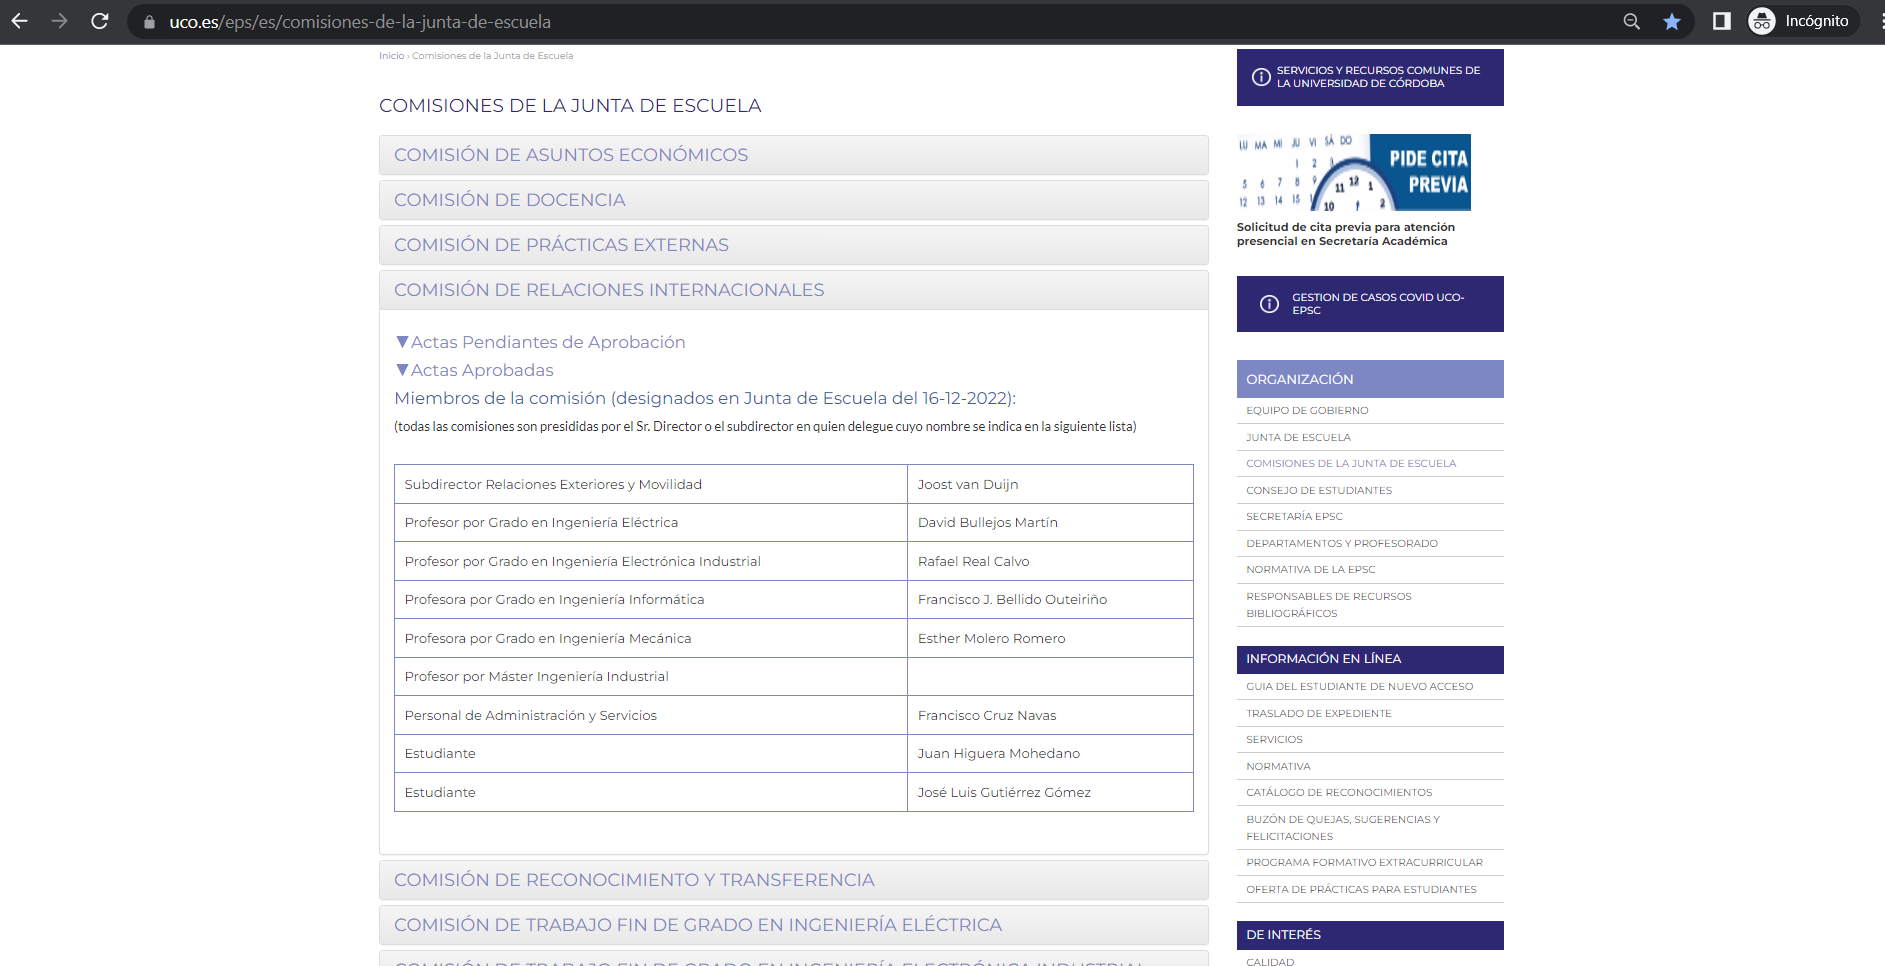
\includegraphics[scale=0.4]{img/capturas/WebComisionesEPSUCO.png}
    \caption{WEB: Información sobre los miembros de las comisiones de la EPS de la UCO}
    \label{fig:WebComisionesEPSUCO}
\end{figure}

\begin{figure}[H]
    \centering
    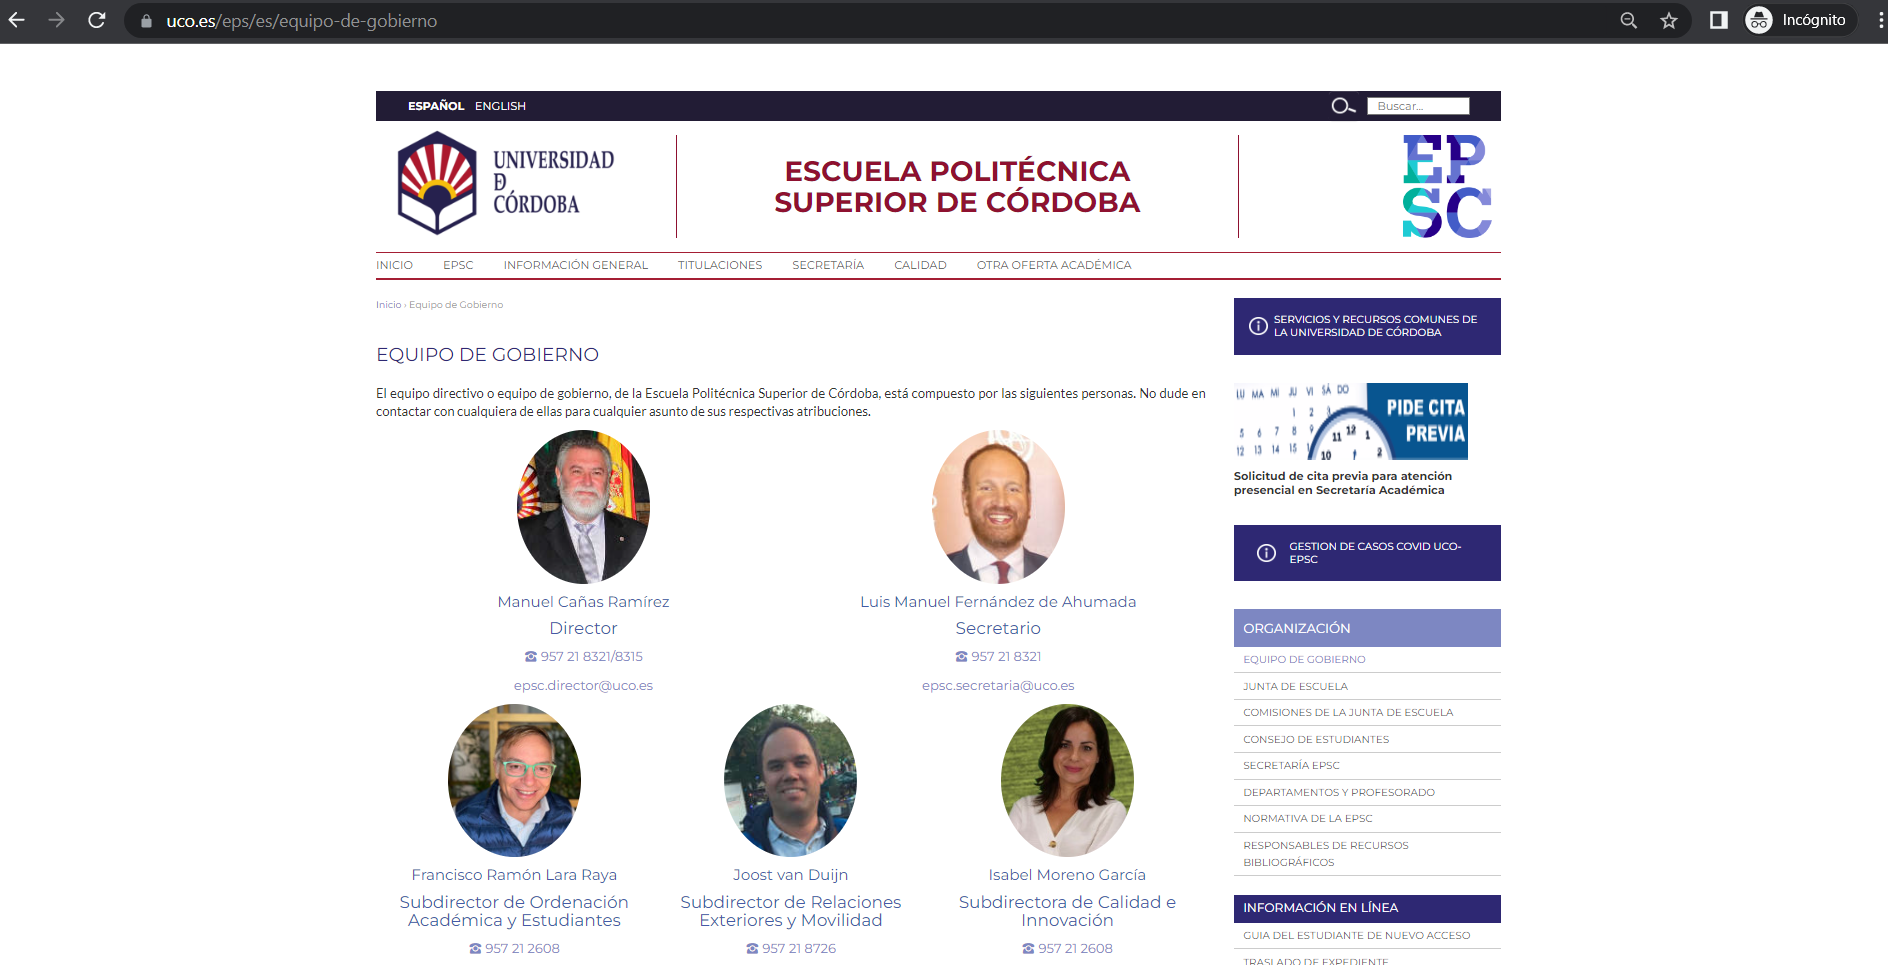
\includegraphics[scale=0.4]{img/capturas/WebEquipoGobiernoEPSUCO.png}
    \caption{WEB: equipo de gobierno de la EPS de la UCO}
    \label{fig:PACE-WebEquipoGobiernoEPSUCO}
\end{figure}

En definitiva, la Universidad de Córdoba carece de una aplicación web con una base de datos que permita asegurar la integridad de la información y evitar datos duplicados, ausentes o incorrectos. En la actualidad, se utilizan páginas web estáticas que deben ser mantenidas de forma individual, lo que provoca una gran carga de trabajo a los administrativos de los centros.

\section{Justificación del Trabajo de Fin de Grado}

El desarrollo del presente Trabajo de Fin de Grado está justificado porque no se tiene conocimiento de ninguna aplicación web que permita la gestión de comisiones de los distintos centros de la Universidad de Córdoba.

Actualmente, se realizan tareas manuales y estáticas sobre estas comisiones que provocan que la gestión administrativa sobre ellas sea una tarea lenta de realizar, sin conseguir una trazabilidad de cada uno de los cambios que pueden producirse a lo largo del tiempo y que repercute directamente en una pérdida de tiempo con respecto a utilizar un sistema que automatice lo máximo posible alguna de sus gestiones.

\chapter{Restricciones} \label{cap:restricciones}

\section{Introducción}

Este capítulo va a describir las restricciones o limitaciones que van a afectar al desarrollo de la aplicación web. 

Las restricciones se pueden clasificar en dos categorías:
\begin{itemize}
    \item Factores iniciales: hacen referencia a la limitaciones impuestas por la propia definición del problema. Estas restricciones no pueden modificarse o eliminarse.
    \item Factores estratégicos: hacen referencia a las diferentes alternativas que se van a considerar para el desarrollo de la aplicación web. En cada caso, se deberá indicar la opción elegida y los motivos de su elección.
\end{itemize}


\section{Factores iniciales} \label{sec:iniciales}

Los factores iniciales,  también conocidos `como ``factores dato'', son limitaciones que que vienen dadas por la naturaleza del problema real. Este tipo de restricciones no se pueden  modificar bajo ningún concepto, ya que entonces eso implicaría abordar un problema nuevo.

Se van a considerar los siguientes factores iniciales:
\begin{itemize}
    \item Se debe desarrollar una aplicación web.
    \item La aplicación web se debe ejecutar en cualquier navegador.
    \item La interfaz debe cumplir con un mínimo de principios de usabilidad que permita ser efectiva, útil, intuitiva, con una estructura consistente, sencilla en su navegación y adaptable a cualquier dispositivo.
    \item Debe contemplar los módulos del usuario público, responsable de la comisión, miembro de la comisión y administrador. 
    \item Se debe garantizar que los datos solamente sean accedidos por aquellos usuarios que tengan la la autorización correspondiente.
    \item El código deberá ser modular para facilitar el mantenimiento y actualización de la aplicación web.
\end{itemize}

Una descripción más detallada de los módulos de los usuarios se mostrará en el Capítulo \ref{cap:especificacion_requisitos} de Especificación de Requisitos.


\section{Factores estratégicos} \label{sec:estrategicos}

Para el desarrollo de la aplicación web, se van a considerar los siguientes factores estratégicos, indicando las alternativas disponibles en cada caso y la opción elegida y los motivos de su elección.


\subsection{Metodología}


Se han considerado diferentes metodologías para el desarrollo de la aplicación web:
\begin{itemize}
    \item  Paradigma de desarrollo de software clásico o ``Modelo en Cascada'' \cite{pressman}:  se caracteriza por el desarrollo lineal de cada una de las fases del proceso de desarrollo. Actualmente, esta metodología se encuentra obsoleta porque no permite desarrollar distintas fases del proyecto sin pasar por todas las anteriores.
    \item Metodología OMT (\textit{Object-Modeling Technique}) \cite{omt}, también denominada ``Paradigma de modelado y diseño orientado a objetos'': esta metodología no se centra en las tareas de cada módulo, sino en la definición de los objetos que se utilicen describiendo sus métodos y atributos. También está en desuso.
    \item Metodologías ágiles como \textit{Scrum} \cite{scrum}, que utiliza iteraciones que desarrollan partes del sistema en periodos cortos de tiempo.
    \item Metodología basada en la notación UML (\textit{Unified modified language})\cite{uml} o ``Lenguaje Unificado de Modelado'':  es un lenguaje de modelado bien definido con una notación estándar para el desarrollo de aplicaciones de software que está amparado por la compañía \textit{Object Management Group} (OMG) \cite{omg}. 
\end{itemize}

Para el proceso de abstracción del mundo real a nuestra aplicación, se utilizarán los diagramas del lenguaje de modelado unificado de sus siglas del inglés UML, la metodología basada en la notación de UML que permite un modelado visual que se comprende con facilidad. Además, está aprobada como estándar internacional por la \textit{International Organization for Standardization} bajo la norma ISO/IEC 19501:2005 \cite{iso19501}. UML proporciona numerosos diagramas para la descripción del proceso de desarrollo del software, como, por ejemplo, el diagrama de casos de uso, que refleja los actores del sistema y los escenarios se ejecutarán, el diagrama de secuencia que muestra cómo el programa realiza una funcionalidad, o el diagrama de clases que refleja las distintas clases, sus propiedades y métodos.


\subsection{Entorno de desarrollo}
El entorno de desarrollo integrado (IDE\footnote{En inglés, \textit{Integrated Development Environment} (IDE).}) es la herramienta utilizada para desarrollar la aplicación. Se han considerado varias alternativas, como son Visual Studio Code \cite{visualStudioCode}, editor de código con múltiples y potentes extensiones, Eclipse \cite{eclipse} o Sublime Text \cite{sublimeText}.

Se ha elegido Visual Studio Code \cite{visualStudioCode} por tener soporte para múltiples lenguajes de programación y contar con extensiones que ayudaran a trabajar aún más rápido.

Como \textit{framework} se ha elegido Laravel\cite{laravel} porque tiene herramientas que facilitan el desarrollo de aplicaciones web e incluye funcionalidades extra como las relacionadas con la seguridad.

\subsection{Base de datos}\label{sec:bases-de-datos}

Laravel\cite{laravel} permite el uso de diferentes sistemas de gestión de bases de datos, como MySql \cite{mysql}, Oracle \cite{oracle} o PostgreSQL \cite{postgreSQL}. Se ha elegido MySql \cite{mysql} por los siguientes motivos:
\begin{itemize}
    \item Software de código abierto y multiplataforma.
    \item Posee una gran conectividad, velocidad y seguridad, siendo muy apropiado para acceder a bases de datos en Internet.
    \item Es uno de los sistemas de gestión de base datos más populares del mundo, sobre todo para el desarrollo de aplicaciones web.
\end{itemize}


\subsection{Lenguaje de programación}

Existen numerosos lenguajes de programación que se pueden utilizar para el desarrollo de aplicaciones web, como PHP \cite{PHP},  Python \cite{python} o Ruby \cite{ruby}. Se ha elegido el lenguaje de programación PHP \cite{PHP} porque es el que utiliza Laravel \cite{laravel}, el \textit{framework} seleccionado. PHP es un lenguaje multiplataforma, interpretado y orientados a objetos, que puede combinarse con código HTML \cite{html}, lenguaje para hojas de estilo CSS \cite{css} y código JavaScript \cite{javascript} para el desarrollo de aplicaciones web.

    
\chapter{Recursos}\label{cap:recursos}

\section{Recursos humanos}
\begin{itemize}
    \item \textbf{Autor}
    \item[] Javier Ruiz Jurado, estudiante del Grado en Ingeniería Informática, especialidad de Ingeniería del Software.
    \item \textbf{Director}
    \item[] José Luis Ávila Jiménez
\end{itemize}

\section{Recursos de hardware}

Para el desarrollo de la aplicación en el entorno local, se va a utilizar el equipo del alumno que tiene las características siguientes:
\begin{itemize}
    \item Ordenador: Acer Nitro 5
    \item Sistema operativo: Windows 11 Professional
    \item RAM instalada: 8GB DDR4
    \item Procesador: Intel(R) Core(TM) i7-10750H CPU @ 2.60GHz 
\end{itemize}

Para el despliegue de la aplicación web, se hará uso de un servidor VPS con las características siguientes:
\begin{itemize}
    \item Platform: Linux x86-64
    \item OS Package: Centos 7 (for AMD64/Intel EM64T) Virtuozzo Template
    \item Memory: 4.00 GB
    \item SSD: 50.00 GB
\end{itemize}


\section{Recursos de software}

Se van a utilizar los siguientes recursos de software para el desarrollo de la aplicación web: 
\begin{itemize}
    \item Editor de código fuente para el desarrollo de la aplicación web: Visual Studio Code \cite{visualStudioCode}
    \item \textit{Framework} utilizado para el desarrollo de la aplicación web, tanto en \textit{Back end} y \textit{Front end}: Laravel \cite{laravel}.
    \item Sistema de gestión de base de datos: MySql \cite{mysql}.
    \item Lenguajes de Programación: PHP \cite{PHP}, JavaScript \cite{javascript}.
    \item Redacción del documento: Overleaf \cite{overleaf}, editor en línea de documentos escritos en \LaTeX. 
    \item Editor de diagramas: draw.io \cite{drawio} y StarUML \cite{starUML}.
    \item Repositorio remoto en Github \cite{github}.
\end{itemize}




\part{Análisis}
\chapter{Especificación de requisitos}\label{cap:especificacion_requisitos}

\section{Introducción}

Se desea desarrollar una aplicación web que permita la la gestión de comisiones de los centros pertenecientes a la Universidad de Córdoba. Las siguientes secciones describen los actores del sistema (Sección \ref{sec:actores}), la descripción modular (Sección \ref{sec:modulos}), los requisitos del sistema (Sección  \ref{sec:requisitos-del-sistema})  y los supuestos semánticos de la información que se van a utilizar (Sección \ref{sec:supuestos-semanticos}).

\section{Actores del sistema}\label{sec:actores}

Se van a considerar los siguientes tipos de usuario en la aplicación web: 
    \begin{itemize}
    \item Público: usuario no registrado en el sistema que podrá consultar la información pública.
    \item Usuario universitario: usuario registrado en el sistema que podrá obtener distintos certificados históricos y actuales sobre la participación como miembro de equipo de gobierno, junta o comisiones a la largo del tiempo.
    \item Responsable de la comisión: usuario registrado en el sistema que será responsable de la gestión de la información de la comisión responsable.
    \item Responsable de junta: usuario registrado en el sistema que será responsable de la gestión de la información de la junta responsable y de todas sus comisiones.
    \item Responsable de centro: usuario registrado en el sistema que será responsable de la gestión de la información todas las comisiones de su centro.
    \item Administrador: usuario registrado en el sistema que tendrá un control completo de la aplicación. En particular, tendrá las competencias exclusivas de la gestión de todos los tipos de usuarios, centros y comisiones. Además, se encargará de la gestión de las copias de seguridad.    
    \end{itemize}

\section{Módulos de la aplicación}\label{sec:modulos}

La aplicación web va a estar compuesta por cuatro módulos que corresponderán a cada uno de los tipos de usuario considerados y que se describen en las siguientes secciones.

\subsection{Módulo del usuario público}

El usuario público podrá consultar toda la información pública que esté disponible:
\begin{itemize}
    \item Consultar la información pública: comisiones de un centro, miembros actuales de una comisión, consulta de actas aprobadas y pendientes de aprobación,...
    \item Consultar la ayuda del usuario público.
\end{itemize}

\subsection{Módulo del usuario universitario}

Además de las acciones disponibles para el usuario público, el usuario universitario podrá desarrollar las siguientes actividades:
\begin{itemize}
    \item Obtención de diferentes tipos certificados (pertenencia a una comisión, comisiones en las cuales ha pertenecido en un rango de fechas...).
    \item Consultar la ayuda del miembro de la comisión.
\end{itemize}

\subsection{Módulo del responsable de la comisión}
Además de las acciones disponibles para el usuario universitario, el responsable de la comisión podrá desarrollar las siguientes actividades:

\begin{itemize}
    \item Consultar, insertar, actualizar y eliminar la información de la comisión responsable.
    \item Asignar/excluir miembros de las comisiones responsables.
    \item Consultar, insertar, actualizar y eliminar la información de las convocatorias de la comisión responsable.
    \item Consultar la ayuda del responsable de comisión.
\end{itemize}

\subsection{Módulo del responsable de junta}
Además de las acciones disponibles para el responsable de la comisión, el responsable de la junta podrá desarrollar las siguientes actividades:
\begin{itemize}
    \item Consultar, insertar, actualizar y eliminar la información de la junta responsable.
    \item Consultar, insertar, actualizar y eliminar la información de las comisiones de la junta.
    \item Asignar/excluir miembros de las juntas del centro responsable.
    \item Asignar/excluir responsable de las comisiones de la junta responsable.
    \item Consultar, insertar, actualizar y eliminar la información de las convocatorias de la junta responsable.
    \item Consultar la ayuda del responsable de junta.
\end{itemize}

\subsection{Módulo del responsable de centro}
Además de las acciones disponibles para el responsable de la junta, el responsable del centro podrá desarrollar las siguientes actividades:
\begin{itemize}
    \item Consultar, insertar, actualizar y eliminar la información del centro responsable.
    \item Consultar, insertar, actualizar y eliminar la información de las juntas del centro.
    \item Asignar/excluir miembros de gobierno del centro responsable.
    \item Asignar/excluir responsable de las juntas del centro responsable.
\item Consultar la ayuda del responsable de centro.
\end{itemize}

\subsection{Módulo del administrador}

El usuario de tipo Administrador tendrá un control total de la aplicación. Además, se encargará de forma exclusiva de los siguientes módulos:
\begin{itemize}
    \item Gestión de usuarios registrados: responsables y miembros de centro, junta y comisión.
    \item Gestión de los centros universitarios.
    \item Gestión de copias de seguridad.
    \item Consultar la ayuda del administrador.
\end{itemize}

En principio, la aplicación solamente tendrá un único administrador.

\section{Requisitos del sistema}\label{sec:requisitos-del-sistema}

Los requisitos del sistema hacen referencia a todas las características relacionadas con la aplicación web. Se describirán los siguientes tipos de requisitos:
\begin{itemize}
    \item Requisitos funcionales: describen las tareas que la aplicación debe realizar para satisfacer las necesidades del problema (Sección \ref{sec:requisitos-funcionales}).
    \item Requisitos no funcionales: describen cómo se tiene que satisfacer las necesidades del problema  (Sección \ref{sec:requisitos-no-funcionales}).
    \item Requisitos de la interfaz: describen cómo debe ser la comunicación entre el usuario y la aplicación  (Sección \ref{sec:requisitos-interfaz}).
    \item Requisitos de la información: describen las características de los datos que se van a gestionar (Sección \ref{sec:requisitos-información}).
\end{itemize}


\subsection{Requisitos funcionales}\label{sec:requisitos-funcionales}

Los requisitos funcionales indican lo que el sistema debe hacer. Cada uno de estos requisitos debe tener dos propiedades: 
\begin{itemize}
    \item Ser completo: el requisito debe mencionar exactamente lo que el sistema debe hacer
    \item Ser cerrado: el requisito debe ser claro y no estar abierto a múltiples interpretaciones, sino solamente a una.
\end{itemize}

Los requisitos funcionales que se van a considerar se agruparán según los módulos de los tipos de usuario y se denotarán como RF-<nº requisito>.

 \begin{itemize}
 \item \textbf{Módulo del usuario público}
 \item[] La aplicación debe permitir que el usuario público pueda realizar las siguientes acciones:
     \begin{itemize}
         \item RF-1. Consultar la información vigente de los miembros del equipo de gobierno de todos los centros de la UCO.
         \item RF-2. Consultar la información vigente de los miembros de las juntas de todos los centros de la UCO.
         \item RF-3. Consultar la información vigente de las comisiones pertenecientes a las juntas de todos los centros de la UCO.
         \item RF-4. Consultar la información vigente de los miembros de las comisiones de las comisiones pertenecientes a las juntas de todos los centros de la UCO.
         \item RF-5. Consultar la información de las convocatorias realizadas de las juntas vigentes de todos los centros de la UCO.
         \item RF-6. Consultar la información de las convocatorias realizadas de las comisiones vigentes de las juntas de todos los centros de la UCO.
         \item RF-7. Consultar la ayuda para el usuario público. 
     \end{itemize}

 \item \textbf{Módulo del usuario universitario}
 \item[] La aplicación debe permitir que el usuario universitario registrado pueda realizar las siguientes acciones: 
     \begin{itemize}
         \item RF-8. Gestionar la información de su perfil.
             \begin{itemize}
                 \item RF-8.1. Modificar la constraseña del usuario.
                 \item RF-8.2. Modificar imagen de usuario.
             \end{itemize}               
         \item RF-9. Obtener diferentes tipos de certificados:
             \begin{itemize}
                 \item RF-9.1. Descarga de certificado de situación actual.
                 \item RF-9.2. Descarga de certificado de centros en los que ha participado como miembro de equipo de gobierno en un periodo de tiempo.
                 \item RF-9.3. Descarga de certificado de certificado de juntas que ha representado en un periodo de tiempo.
                 \item RF-9.4. Descarga de certificado de comisiones a las que ha pertenecido en un periodo de tiempo.
                  \item RF-9.4. Descarga de certificado de convocatorias de junta o comisión a las que ha asistido en un periodo de tiempo.
             \end{itemize}            
         \item RF-10. Consultar la ayuda para usuario universitario.
     \end{itemize}

 \item \textbf{Módulo del responsable de comisión}
 \item[] La aplicación debe permitir que el responsable de comisión en activo pueda realizar las siguientes acciones:
     \begin{itemize}
         \item RF-11. Gestionar los miembros de la comisión responsable.
             \begin{itemize}
                  \item RF-11.1. Crear un miembro de comisión.
                  \item RF-11.2. Buscar un miembro de comisión.
                  \item RF-11.3. Consultar un miembro de comisión.
                  \item RF-11.4. Modificar un miembro de comisión.
                  \item RF-11.5. Eliminar un miembro de comisión.
                  \item RF-11.6. Asignar/desasignar miembro responsable de comisión.
             \end{itemize} 
         \item RF-12. Gestionar las convocatorias de la comisión.
             \begin{itemize}
                  \item RF-12.1. Crear una convocatoria de comisión.
                  \item RF-12.2. Buscar una convocatoria de comisión.
                  \item RF-12.3. Consultar una convocatoria de comisión.
                  \item RF-12.4. Modificar una convocatoria de comisión.
                  \item RF-12.5. Eliminar una convocatoria de comisión.
                  \item RF-12.6. Asignar miembros a una convocatoria de comisión.
                  \item RF-12.7. Desasignar miembros una convocatoria de comisión.
             \end{itemize} 
         \item RF-13. Consultar la ayuda para el responsable de comisión.
     \end{itemize}

\item \textbf{Módulo del responsable de junta}
 \item[] La aplicación debe permitir que el responsable de junta en activo pueda realizar las siguientes acciones:
     \begin{itemize}
        \item RF-14. Gestionar los miembros de la junta responsable.
             \begin{itemize}
                  \item RF-14.1. Crear un miembro de junta.
                  \item RF-14.2. Buscar un miembro de junta.
                  \item RF-14.3. Consultar un miembro de junta.
                  \item RF-14.4. Modificar un miembro de junta.
                  \item RF-14.5. Eliminar un miembro de junta.
                  \item RF-14.6. Asignar/desasignar miembro responsable de junta.
             \end{itemize}  
         \item RF-15. Gestionar las  comisiones de la junta responsable.
             \begin{itemize}
                  \item RF-15.1. Crear una comisión.
                  \item RF-15.2. Buscar una comisión.
                  \item RF-15.3. Consultar una comisión.
                  \item RF-15.4. Modificar una comisión.
                  \item RF-15.5. Eliminar una comisión.
             \end{itemize}    
          \item RF-16. Gestionar los miembros de todas las comisiones de la junta responsable.
             \begin{itemize}
                  \item RF-16.1. Crear un miembro de comisión.
                  \item RF-16.2. Buscar un miembro de comisión.
                  \item RF-16.3. Consultar un miembro de comisión.
                  \item RF-16.4. Modificar un miembro de comisión.
                  \item RF-16.5. Eliminar un miembro de comisión.
                  \item RF-16.6. Asignar/desasignar miembro responsable de comisión.
             \end{itemize} 
             
             \item RF-17. Gestionar las convocatorias de la junta responsable.
             \begin{itemize}
                  \item RF-17.1. Crear una convocatoria de junta.
                  \item RF-17.2. Buscar una convocatoria de junta.
                  \item RF-17.3. Consultar una convocatoria de junta.
                  \item RF-17.4. Modificar una convocatoria de junta.
                  \item RF-17.5. Eliminar una convocatoria de junta.
                  \item RF-17.6. Asignar miembros a una convocatoria de junta.
                  \item RF-17.7. Desasignar miembros una convocatoria de junta.
             \end{itemize}
          \item RF-18. Gestionar las convocatorias de todas las comisiones de la junta responsable.
             \begin{itemize}
                  \item RF-18.1. Crear una convocatoria de comisión.
                  \item RF-18.2. Buscar una convocatoria de comisión.
                  \item RF-18.3. Consultar una convocatoria de comisión.
                  \item RF-18.4. Modificar una convocatoria de comisión.
                  \item RF-18.5. Eliminar una convocatoria de comisión.
                  \item RF-18.6. Asignar miembros a una convocatoria de comisión.
                  \item RF-18.7. Desasignar miembros una convocatoria de comisión.
             \end{itemize} 
         \item RF-19. Consultar la ayuda para el responsable de junta.
     \end{itemize}

\item \textbf{Módulo del responsable de centro}
 \item[] La aplicación debe permitir que el responsable de centro en activo pueda realizar las siguientes acciones:
     \begin{itemize}
         \item RF-20. Gestionar los miembros de gobierno del centro responsable.
             \begin{itemize}
                  \item RF-20.1. Crear un miembro de gobierno.
                  \item RF-20.2. Buscar un miembro de gobierno.
                  \item RF-20.3. Consultar un miembro de gobierno.
                  \item RF-20.4. Modificar un miembro de gobierno.
                  \item RF-20.5. Eliminar un miembro de gobierno.
                 \item RF-20.6. Asignar/desasignar miembro responsable de centro.
             \end{itemize} 
        \item RF-21. Gestionar las juntas del centro responsable.
             \begin{itemize}
                  \item RF-21.1. Crear una junta.
                  \item RF-21.2. Buscar una junta.
                  \item RF-21.3. Consultar una junta.
                  \item RF-21.4. Modificar una junta.
                  \item RF-21.5. Eliminar una junta.
             \end{itemize} 
        \item RF-22. Gestionar los miembros todas las juntas del centro responsable.
             \begin{itemize}
                  \item RF-22.1. Crear un miembro de junta.
                  \item RF-22.2. Buscar un miembro de junta.
                  \item RF-22.3. Consultar un miembro de junta.
                  \item RF-22.4. Modificar un miembro de junta.
                  \item RF-22.5. Eliminar un miembro de junta.
                  \item RF-22.6. Asignar/desasignar miembro responsable de junta.
             \end{itemize}  
         \item RF-23. Gestionar las convocatorias de todas las juntas del centro responsable.
             \begin{itemize}
                  \item RF-23.1. Crear una convocatoria de junta.
                  \item RF-23.2. Buscar una convocatoria de junta.
                  \item RF-23.3. Consultar una convocatoria de junta.
                  \item RF-23.4. Modificar una convocatoria de junta.
                  \item RF-23.5. Eliminar una convocatoria de junta.
                  \item RF-23.6. Asignar miembros a una convocatoria de junta.
                  \item RF-23.7. Desasignar miembros una convocatoria de junta.
             \end{itemize}
        \item RF-24. Gestionar todas las comisiones de todas las juntas del centro responsable.
             \begin{itemize}
                  \item RF-24.1. Crear una comisión.
                  \item RF-24.2. Buscar una comisión.
                  \item RF-24.3. Consultar una comisión.
                  \item RF-24.4. Modificar una comisión.
                  \item RF-24.5. Eliminar una comisión.
             \end{itemize}    
          \item RF-25. Gestionar los miembros de todas las comisiones de todas las juntas del centro responsable.
             \begin{itemize}
                  \item RF-25.1. Crear un miembro de comisión.
                  \item RF-25.2. Buscar un miembro de comisión.
                  \item RF-25.3. Consultar un miembro de comisión.
                  \item RF-25.4. Modificar un miembro de comisión.
                  \item RF-25.5. Eliminar un miembro de comisión.
                  \item RF-25.6. Asignar/desasignar miembro responsable de comisión.
             \end{itemize} 
        \item RF-26. Gestionar las convocatorias de todas las comisiones de todas las juntas del centro responsable.
             \begin{itemize}
                  \item RF-26.1. Crear una convocatoria de comisión.
                  \item RF-26.2. Buscar una convocatoria de comisión.
                  \item RF-26.3. Consultar una convocatoria de comisión.
                  \item RF-26.4. Modificar una convocatoria de comisión.
                  \item RF-26.5. Eliminar una convocatoria de comisión.
                  \item RF-26.6. Asignar miembros a una convocatoria de comisión.
                  \item RF-26.7. Desasignar miembros una convocatoria de comisión.
             \end{itemize}
         \item RF-27. Consultar la ayuda para el responsable de centro.
     \end{itemize}

 \item \textbf{Módulo del administrador}
 \item[] La aplicación debe permitir que el administrador pueda realizar las siguientes acciones:
     \begin{itemize}
        \item RF-28. Gestionar los centros de la UCO.
             \begin{itemize}
                  \item RF-28.1. Crear un centro.
                  \item RF-28.2. Buscar un centro.
                  \item RF-28.3. Consultar un centro.
                  \item RF-28.4. Modificar un centro.
                  \item RF-28.5. Eliminar un centro.
             \end{itemize} 
        \item RF-29. Gestionar los miembros de gobierno de todos los centros.
             \begin{itemize}
                  \item RF-29.1. Crear un miembro de gobierno.
                  \item RF-29.2. Buscar un miembro de gobierno.
                  \item RF-29.3. Consultar un miembro de gobierno.
                  \item RF-29.4. Modificar un miembro de gobierno.
                  \item RF-29.5. Eliminar un miembro de gobierno.
                 \item RF-29.6. Asignar/desasignar miembro responsable de centro.
             \end{itemize} 
         \item RF-30. Gestionar las juntas de todos los centros.
             \begin{itemize}
                  \item RF-30.1. Crear una junta.
                  \item RF-30.2. Buscar una junta.
                  \item RF-30.3. Consultar una junta.
                  \item RF-30.4. Modificar una junta.
                  \item RF-30.5. Eliminar una junta.
             \end{itemize} 
        \item RF-31. Gestionar los miembros todas las juntas de todos los centros.
             \begin{itemize}
                  \item RF-31.1. Crear un miembro de junta.
                  \item RF-31.2. Buscar un miembro de junta.
                  \item RF-31.3. Consultar un miembro de junta.
                  \item RF-31.4. Modificar un miembro de junta.
                  \item RF-31.5. Eliminar un miembro de junta.
                  \item RF-31.6. Asignar/desasignar miembro responsable de junta.
             \end{itemize}
        \item RF-32. Gestionar las convocatorias de todas las juntas de todos los centros.
             \begin{itemize}
                  \item RF-32.1. Crear una convocatoria de junta.
                  \item RF-32.2. Buscar una convocatoria de junta.
                  \item RF-32.3. Consultar una convocatoria de junta.
                  \item RF-32.4. Modificar una convocatoria de junta.
                  \item RF-32.5. Eliminar una convocatoria de junta.
                  \item RF-32.6. Asignar miembros a una convocatoria de junta.
                  \item RF-32.7. Desasignar miembros una convocatoria de junta.
             \end{itemize}
        \item RF-33. Gestionar todas las comisiones de todas las juntas de todos los centros.
             \begin{itemize}
                  \item RF-33.1. Crear una comisión.
                  \item RF-33.2. Buscar una comisión.
                  \item RF-33.3. Consultar una comisión.
                  \item RF-33.4. Modificar una comisión.
                  \item RF-33.5. Eliminar una comisión.
             \end{itemize}    
          \item RF-34. Gestionar los miembros de todas las comisiones de todas las juntas de todos los centros.
             \begin{itemize}
                  \item RF-34.1. Crear un miembro de comisión.
                  \item RF-34.2. Buscar un miembro de comisión.
                  \item RF-34.3. Consultar un miembro de comisión.
                  \item RF-34.4. Modificar un miembro de comisión.
                  \item RF-34.5. Eliminar un miembro de comisión.
                  \item RF-34.6. Asignar/desasignar miembro responsable de comisión.
             \end{itemize} 
        \item RF-35. Gestionar las convocatorias de todas las comisiones de todas las juntas de todos los centros.
             \begin{itemize}
                  \item RF-35.1. Crear una convocatoria de comisión.
                  \item RF-35.2. Buscar una convocatoria de comisión.
                  \item RF-35.3. Consultar una convocatoria de comisión.
                  \item RF-35.4. Modificar una convocatoria de comisión.
                  \item RF-35.5. Eliminar una convocatoria de comisión.
                  \item RF-35.6. Asignar miembros a una convocatoria de comisión.
                  \item RF-35.7. Desasignar miembros una convocatoria de comisión.
             \end{itemize}
         \item RF-36. Consultar la ayuda para el administrador.
         \item RF-37. Gestionar los usuario de la UCO.
             \begin{itemize}
                  \item RF-37.1. Crear un usuario.
                  \item RF-37.2. Buscar un usuario.
                  \item RF-37.3. Consultar un usuario.
                  \item RF-37.4. Modificar un usuario.
                  \item RF-37.5. Eliminar un usuario.
             \end{itemize} 
     \end{itemize}
 \end{itemize}

\subsection{Requisitos no funcionales}\label{sec:requisitos-no-funcionales}

Los requisitos no funcionales representan cómo tiene que trabajar la aplicación. Los requisitos no funcionales se denotarán como RNF-<nº requisito>.

\begin{itemize}
    \item RNF-1. La aplicación debe tener una interfaz gráfica que sea fácil de usar y amigable para el usuario.
    \item RNF-2. La aplicación debe ser robusta y adaptable a cualquier dispositivo.
    \item RNF-3. La aplicación deberá funcionar correctamente en los principales navegadores web.
    \item RNF-4. Los usuarios registrados en el sistema deberán identificarse con nombre de usuario y contraseña para acceder.
    \item RNF-5. La aplicación solamente tendrá un usuario con el rol de administrador.
    \item RNF-6. El borrado de todos registros en la base de datos serán borrados lógicos (soft delete), mediante actualización de un campo.
\end{itemize}


\subsection{Requisitos de la interfaz}\label{sec:requisitos-interfaz}
  
  La interfaz es el dispositivo que permite la comunicación entre el usuario y el sistema. En esta sección, se enumeran los requisitos que debe tener la interfaz para que pueda ser utilizada por todos los tipos de usuario.
  
  Los requisitos la interfaz  especifican cómo deber la comunicación entre el usuario y la parte visible de la aplicación. Se denotarán como RINT-<nº de requisito> 


\begin{itemize}
    \item RINT-1. La interfaz debe ser gráfica, intuitiva, sencilla y agradable para el usuario.
    \item RINT-2. La nomenclatura que usará la interfaz para mostrar la información y las distintas opciones al usuario será la más clara posible.
    \item RINT-3.La interfaz utilizará menús para mostrar la información correspondiente a cada tipo de usuario.    
    \item RINT-4.La interfaz utilizará menús para mostrar la información correspondiente a cada tipo de usuario.
    \item RINT-5. La interfaz utilizará diferentes tipos de mensajes: informativos, de error, de confirmación, etc.
    \item RINT-6. La interfaz utilizará formularios para pedir al usuario la información que corresponda, resaltando aquellos campos que sean obligatorios.
\end{itemize}

\subsection{Requisitos de información}\label{sec:requisitos-información}

Los requisitos de información hacen referencia a los datos que debe gestionar la aplicación web. Se denotarán como RI-<no de requisito>.

Se deberá almacenar la siguiente información:
\begin{itemize}
    \item RI-1. Usuarios registrados: responsables de centros, de juntas, de comisiones y usuarios universitarios. Para cada usuario, se deberá almacenar como mínimo su nombre, email y contraseña.
    \item RI-2. Centros: facultades, escuelas y centros adscritos.
    \item RI-3. Juntas: fecha de constitución, fecha disolución.
    \item RI-4. Comisiones: comisión de Asuntos Económicos, comisión de Docencia, comisión de Ordenación Académica, comisión de Relaciones Exteriores, comisión de Reconocimientos y Convalidaciones, comisión Académica de los Másteres, unidades de Garantía de Calidad...
    \item RI-5. Convocatorias: ordinaria, extraordinaria, urgente.
    \item RI-6. Miembros de gobierno: director, secretario, vicedirector, subdirector.
    \item RI-7. Miembros de junta: Profesorado vinculación permanente, otro personal docente e investigador y  PAS, alumnado, personal libre designación.
    \item RI-8. Miembros de comisión: Profesorado vinculación permanente, otro personal docente e investigador y  PAS, alumnado, personal libre designación.
\end{itemize}

        
Una descripción más detallada de la información que se va a gestionar se puede consultar en la sección \ref{sec:supuestos-semanticos} de Supuestos Semánticos y en el capítulo \ref{cap:modelo_de_datos} de Modelo de Datos.

 \section{Supuestos semánticos}\label{sec:supuestos-semanticos}

Una vez descritos los requisitos funcionales, de información y de interfaz, los supuestos semánticos que se definen a continuación describen de manera más formal y precisa las restricciones identificadas en la definición del problema.

\chapter{Modelo de datos} \label{cap:modelo_de_datos}

\section{Introducción}

En este capítulo se describirá conceptualmente el modelo de datos que empleará el
sistema. Se identificarán las entidades que intervienen en el problema, sus atributos y las interrelaciones entre dichas entidades.

Para la confección del modelo, se empleará la notación del Modelo Entidad - Interrelación (modelo E-R) propuesto por Peter Chen\cite{peter}. El esquema E-R describe la información representando los distintos elementos que la componen mediante un conjunto limitado de símbolos y reglas de relación entre ellos. Básicamente, los elementos principales del modelo son “tipo de entidad” y “tipo de interrelación”.

En las siguientes secciones se especifican con detalle los tipos de entidad y los tipos de interrelación que intervienen en el modelo, y se mostrará el diagrama E-R completo, que ofrecerá una visión global del problema.

\section{Tipos de entidad} \label{sec:entidades}

De acuerdo con el modelo E-R, un tipo de entidad representa a una serie de entes,
objetos o personas reales o abstractos que forman parte del universo del problema a
describir. Los tipos de entidad pueden ser fuertes o débiles.

\begin{itemize}

    \item Tipo de entidad fuerte: su existencia no depende de la de otro tipo de entidad.

    \item Tipo de entidad débil: su existencia depende de la de otro tipo de entidad. La debilidad puede ser por existencia o por identificación.

    \begin{itemize}
        \item Tipo de entidad débil por existencia: puede ser identificado por sí mismo a partir de sus atributos propios, pero requiere de la existencia de otro tipo de entidad del que depende.

        \item Tipo de entidad débil por identificación: es un tipo de entidad débil por existencia que, además, requiere de algún atributo identificativo del tipo de entidad del que depende para poder ser identificado y diferenciado.
    \end{itemize} 
\end{itemize}    

Las entidades de un determinado tipo de entidad se describen mediante un conjunto
de atributos que representan cada una de las características o propiedades que lo describen.

Cada atributo tiene asociado un dominio de valores permitidos. Cada entidad se identifica y diferencia de forma inequívoca mediante un atributo identificador, que toma un valor único para cada entidad.

En esta sección se describirán todos los tipos de entidad que se han identificado
que forman parte del problema descrito, indicando para cada uno de ellos la siguiente
información:

\begin{itemize}
    \item Descripción: definición de la entidad y función dentro del universo del problema.
    
    \item Restricción: indicación de si tiene alguna debilidad por identificación o existencia respecto de otra entidad.
    
    \item Características: se indicarán las siguientes: 
    \begin{itemize}
        \item Nombre del tipo de entidad.
        \item Tipo: Fuerte o débil.
        \item Atributos heredados.
        \item Atributo identificador primario.
        \item Atributo identificador alternativo.
        \item Número de atributos, incluyendo los heredados.
    \end{itemize}
    
    \item Atributos propios: por cada atributo, además del nombre del mismo, se indicará:
    \begin{itemize}
        \item Definición: descripción del atributo.
        \item Dominio: tipo de dato o valores que puede tomar el atributo.
        \item Tipo: indicación de si es clave primaria o alterna, en su caso, atributo simple, etc.
        \item Opcional: indicación de si el atributo puede contener un valor nulo o no.
        \item Ejemplo: valor de muestra.
    \end{itemize}
    
    \item Diagrama: representación gráfica del tipo de entidad, de acuerdo con la notación E-R.
    
    \item Ejemplo de entidad.
\end{itemize}    

Los tipos de entidad que se han identificado y que se describirán a continuación son los siguientes:
\begin{itemize}
    \item Tipo de entidad: Centro.
    \item Tipo de entidad: Tipo Centro.
    \item Tipo de entidad: Usuario.
    \item Tipo de entidad: Miembro Gobierno.
    \item Tipo de entidad: Tipo Representación Gobierno.
    \item Tipo de entidad: Junta.
    \item Tipo de entidad: Miembro Junta.
    \item Tipo de entidad: Tipo Representación.
    \item Tipo de entidad: Comisión.
    \item Tipo de entidad: Miembro Comisión.
    \item Tipo de entidad: Convocatoria.
    \item Tipo de entidad: Tipo Convocatoria.
    \item Tipo de entidad: Asistente.
\end{itemize}

\subsection{Entidad Tipo Centro}
\begin{itemize}
    \item Descripción: este tipo de entidad representa a los tipos de centros registrados en el sistema que tienen vinculación con la Universidad de Córdoba. Los más destacados serían Escuela, Facultad,...
    \item Restricciones: es una entidad fuerte por lo que no depende de otro tipo de entidad.
    \item Características:
    \begin{itemize}
        \item Nombre de la entidad: Tipo Centro.
        \item Tipo: fuerte.
        \item Atributos heredados: ninguno.
        \item Atributo identificador primario: id.
        \item Atributo identificador alternativo: ninguno.
        \item Número de atributos: 3 (3 propios).
    \end{itemize}

    \item Atributos propios:
    \begin{itemize}
        \item id
        \begin{itemize}
            \item Definición: código numérico secuencial e incremental que identifica el tipo de centro.
            \item Dominio: números enteros mayores que 0.
            \item Tipo: clave primaria.
            \item Opcional: no
            \item Ejemplo: 5
        \end{itemize}

        \item nombre
        \begin{itemize}
            \item Definición: nombre que identifica al tipo de centro.
            \item Dominio: conjunto de 100 caracteres.
            \item Tipo: atributo simple.
            \item Opcional: no
            \item Ejemplo: Escuela
        \end{itemize}

        \item estado
        \begin{itemize}
            \item Definición: estado del tipo de centro.
            \item Dominio: 1 (Habilitado), 0 (Deshabilitado).
            \item Tipo: atributo simple.
            \item Opcional: no
            \item Ejemplo: 1
        \end{itemize}
    \end{itemize}

    \item Diagrama (Figura \ref{fig:E-TipoCentro}):

    \begin{figure}[H]
        \centering
        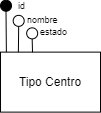
\includegraphics[scale=0.8]{img/diagramas/EER/E-TipoCentro.png}
        \caption{Entidad Tipo Centro}
        \label{fig:E-TipoCentro}
    \end{figure}

    \item Ejemplo de entidad (Tabla \ref{table:T-TipoCentro}):

    \begin{table}[H]
    \centering
        \begin{tabular}{ |p{6cm}||p{6cm}|  }
             \hline
                \multicolumn{2}{|c|}{\textbf{Tipo Centro}} \\
             \hline
                 \textbf{Atributo} & \textbf{Valor} \\
             \hline
                 id & 1 \\
             \hline
                 nombre & Facultad \\
             \hline
                 estado & 1 \\
        \end{tabular}
        \caption{Ejemplo de la entidad \textit{Tipo Centro}}
        \label{table:T-TipoCentro}
    \end{table}
\end{itemize}

\subsection{Entidad TipoRepresentaciónGobierno}
\begin{itemize}
    \item Descripción: este tipo de entidad representa a los tipos de miembros de gobierno registrados en el sistema que tienen vinculación con la Universidad de Córdoba. Los más destacados serían Director o Decano, Secretario, ViceDirectores o Vicedecanos, secretarios dirección...
    \item Restricciones: es una entidad fuerte por lo que no depende de otro tipo de entidad.
    \item Características:
    \begin{itemize}
        \item Nombre de la entidad: TipoRepresentaciónGobierno.
        \item Tipo: fuerte.
        \item Atributos heredados: ninguno.
        \item Atributo identificador primario: id.
        \item Atributo identificador alternativo: ninguno.
        \item Número de atributos: 3 (3 propios).
    \end{itemize}

    \item Atributos propios:
    \begin{itemize}
        \item id
        \begin{itemize}
            \item Definición: código numérico secuencial e incremental que identifica el tipo de centro.
            \item Dominio: números enteros mayores que 0.
            \item Tipo: clave primaria.
            \item Opcional: no
            \item Ejemplo: 5
        \end{itemize}

        \item nombre
        \begin{itemize}
            \item Definición: nombre que identifica al tipo de miembro de gobierno.
            \item Dominio: conjunto de 100 caracteres.
            \item Tipo: atributo simple.
            \item Opcional: no
            \item Ejemplo: Secretario
        \end{itemize}

        \item estado
        \begin{itemize}
            \item Definición: estado del tipo de representación del gobierno.
            \item Dominio: 1 (Habilitado), 0 (Deshabilitado).
            \item Tipo: atributo simple.
            \item Opcional: no
            \item Ejemplo: 1
        \end{itemize}
    \end{itemize}

    \item Diagrama (Figura \ref{fig:E-TipoRepresentaciónGobierno}):

    \begin{figure}[H]
        \centering
        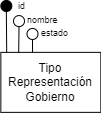
\includegraphics[scale=0.8]{img/diagramas/EER/E-TipoRepresentaciónGobierno.png}
        \caption{Entidad TipoRepresentaciónGobierno}
        \label{fig:E-TipoRepresentaciónGobierno}
    \end{figure}

    \item Ejemplo de entidad (Tabla \ref{table:T-TipoRepresentaciónGobierno}):

    \begin{table}[H]
    \centering
        \begin{tabular}{ |p{6cm}||p{6cm}|  }
             \hline
                \multicolumn{2}{|c|}{\textbf{TipoRepresentaciónGobierno}} \\
             \hline
                 \textbf{Atributo} & \textbf{Valor} \\
             \hline
                 id & 1 \\
             \hline
                 nombre & Secretario \\
             \hline
                 estado & 1 \\
        \end{tabular}
        \caption{Ejemplo de la entidad \textit{TipoRepresentaciónGobierno}}
        \label{table:T-TipoRepresentaciónGobierno}
    \end{table}
\end{itemize}

\subsection{Entidad TipoRepresentaciónGeneral}
\begin{itemize}
    \item Descripción: este tipo de entidad representa a los tipos de miembros de junta y comisión registrados en el sistema que tienen vinculación con la Universidad de Córdoba. Los más destacados serían Profesorado vinculación permanente, otro personal docente e investigador y  PAS, alumnado, personal libre designación...
    \item Restricciones: es una entidad fuerte por lo que no depende de otro tipo de entidad.
    \item Características:
    \begin{itemize}
        \item Nombre de la entidad: TipoRepresentaciónGeneral.
        \item Tipo: fuerte.
        \item Atributos heredados: ninguno.
        \item Atributo identificador primario: id.
        \item Atributo identificador alternativo: ninguno.
        \item Número de atributos: 3 (3 propios).
    \end{itemize}

    \item Atributos propios:
    \begin{itemize}
        \item id
        \begin{itemize}
            \item Definición: código numérico secuencial e incremental que identifica el tipo de centro.
            \item Dominio: números enteros mayores que 0.
            \item Tipo: clave primaria.
            \item Opcional: no
            \item Ejemplo: 5
        \end{itemize}

        \item nombre
        \begin{itemize}
            \item Definición: nombre que identifica al tipo de miembro de junta o comisión.
            \item Dominio: conjunto de 100 caracteres.
            \item Tipo: atributo simple.
            \item Opcional: no
            \item Ejemplo: PAS
        \end{itemize}

        \item estado
        \begin{itemize}
            \item Definición: estado del tipo de representación general.
            \item Dominio: 1 (Habilitado), 0 (Deshabilitado).
            \item Tipo: atributo simple.
            \item Opcional: no
            \item Ejemplo: 1
        \end{itemize}
    \end{itemize}

    \item Diagrama (Figura \ref{fig:E-TipoRepresentaciónGeneral}):

    \begin{figure}[H]
        \centering
        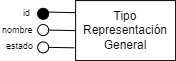
\includegraphics[scale=0.8]{img/diagramas/EER/E-TipoRepresentaciónGeneral.png}
        \caption{Entidad TipoRepresentaciónGeneral}
        \label{fig:E-TipoRepresentaciónGeneral}
    \end{figure}

    \item Ejemplo de entidad (Tabla \ref{table:T-TipoRepresentaciónGeneral}):

    \begin{table}[H]
    \centering
        \begin{tabular}{ |p{6cm}||p{6cm}|  }
             \hline
                \multicolumn{2}{|c|}{\textbf{TipoRepresentaciónGeneral}} \\
             \hline
                 \textbf{Atributo} & \textbf{Valor} \\
             \hline
                 id & 1 \\
             \hline
                 nombre & PAS \\
             \hline
                 estado & 1 \\
        \end{tabular}
        \caption{Ejemplo de la entidad \textit{TipoRepresentaciónGeneral}}
        \label{table:T-TipoRepresentaciónGeneral}
    \end{table}
\end{itemize}

\subsection{Entidad TipoConvocatoria}
\begin{itemize}
    \item Descripción: este tipo de entidad representa a los tipos de convocatorias de junta y comisión registrados en el sistema que tienen vinculación con la Universidad de Córdoba. Los más destacados serían oridnaria, extraordinaria y urgente.
    \item Restricciones: es una entidad fuerte por lo que no depende de otro tipo de entidad.
    \item Características:
    \begin{itemize}
        \item Nombre de la entidad: TipoConvocatoria.
        \item Tipo: fuerte.
        \item Atributos heredados: ninguno.
        \item Atributo identificador primario: id.
        \item Atributo identificador alternativo: ninguno.
        \item Número de atributos: 3 (3 propios).
    \end{itemize}

    \item Atributos propios:
    \begin{itemize}
        \item id
        \begin{itemize}
            \item Definición: código numérico secuencial e incremental que identifica el tipo de centro.
            \item Dominio: números enteros mayores que 0.
            \item Tipo: clave primaria.
            \item Opcional: no
            \item Ejemplo: 5
        \end{itemize}

        \item nombre
        \begin{itemize}
            \item Definición: nombre que identifica al tipo de convocatoria de junta o comisión.
            \item Dominio: conjunto de 100 caracteres.
            \item Tipo: atributo simple.
            \item Opcional: no
            \item Ejemplo: Ordinaria
        \end{itemize}

        \item estado
        \begin{itemize}
            \item Definición: estado del tipo de convocatoria.
            \item Dominio: 1 (Habilitado), 0 (Deshabilitado).
            \item Tipo: atributo simple.
            \item Opcional: no
            \item Ejemplo: 1
        \end{itemize}
    \end{itemize}

    \item Diagrama (Figura \ref{fig:E-TipoConvocatoria}):

    \begin{figure}[H]
        \centering
        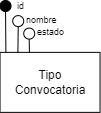
\includegraphics[scale=0.8]{img/diagramas/EER/E-TipoConvocatoria.png}
        \caption{Entidad TipoConvocatoria}
        \label{fig:E-TipoConvocatoria}
    \end{figure}

    \item Ejemplo de entidad (Tabla \ref{table:T-TipoConvocatoria}):

    \begin{table}[H]
    \centering
        \begin{tabular}{ |p{6cm}||p{6cm}|  }
             \hline
                \multicolumn{2}{|c|}{\textbf{TipoConvocatoria}} \\
             \hline
                 \textbf{Atributo} & \textbf{Valor} \\
             \hline
                 id & 1 \\
             \hline
                 nombre & Ordinaria \\
             \hline
                 estado & 1 \\
        \end{tabular}
        \caption{Ejemplo de la entidad \textit{TipoConvocatoria}}
        \label{table:T-TipoConvocatoria}
    \end{table}
\end{itemize}

\subsection{Entidad Usuario}
\begin{itemize}
    \item Descripción: este tipo de entidad representa a los usuarios registrados en el sistema que tienen vinculación con la Universidad de Córdoba.
    \item Restricciones: es una entidad fuerte por lo que no depende de otro tipo de entidad.
    \item Características:
    \begin{itemize}
        \item Nombre de la entidad: Usuario.
        \item Tipo: fuerte.
        \item Atributos heredados: ninguno.
        \item Atributo identificador primario: id.
        \item Atributo identificador alternativo: ninguno.
        \item Número de atributos: 5 propios.
    \end{itemize}

    \item Atributos propios:
    \begin{itemize}
        \item id
        \begin{itemize}
            \item Definición: código numérico secuencial e incremental que identifica el centro.
            \item Dominio: números enteros mayores que 0.
            \item Tipo: clave primaria.
            \item Opcional: no
            \item Ejemplo: 13
        \end{itemize}

        \item name
        \begin{itemize}
            \item Definición: nombre que identifica al usuario.
            \item Dominio: conjunto de 150 caracteres.
            \item Tipo: atributo simple.
            \item Opcional: no
            \item Ejemplo: Javier Ruiz
        \end{itemize}

        \item email
        \begin{itemize}
            \item Definición: dirección de correo del usuario.
            \item Dominio: conjunto de 250 caracteres.
            \item Tipo: atributo simple.
            \item Opcional: no
            \item Ejemplo: i03mosa@uco.es
        \end{itemize}

        \item password
        \begin{itemize}
            \item Definición: contraseña del usuario.
            \item Dominio: conjunto de 250 caracteres encriptados.
            \item Tipo: atributo simple.
            \item Opcional: no
            \item Ejemplo: 2y1092IXUNpkjO0rOQ5byMi
        \end{itemize}

        \item estado
        \begin{itemize}
            \item Definición: estado del usuario.
            \item Dominio: 1 (Habilitado), 0 (Deshabilitado).
            \item Tipo: atributo simple.
            \item Opcional: no
            \item Ejemplo: 1
        \end{itemize}
    \end{itemize}

    \item Diagrama (Figura \ref{fig:E-Usuario}):

    \begin{figure}[H]
        \centering
        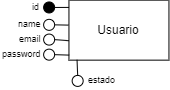
\includegraphics[scale=0.8]{img/diagramas/EER/E-Usuario.png}
        \caption{Entidad Usuario}
        \label{fig:E-Usuario}
    \end{figure}

    \item Ejemplo de entidad (Tabla \ref{table:T-Usuario}):

    \begin{table}[H]
    \centering
        \begin{tabular}{ |p{6cm}||p{6cm}|  }
             \hline
                \multicolumn{2}{|c|}{\textbf{Usuario}} \\
             \hline
                 \textbf{Atributo} & \textbf{Valor} \\
             \hline
                 id & 1 \\
             \hline
                 nombre & Ciencias \\
             \hline
                 email & i03mosa@uco.es \\
            \hline
                 password & 2y1092IXUNpkjO0rOQ5byMi \\
             \hline
                 estado & 1 \\
        \end{tabular}
        \caption{Ejemplo de la entidad \textit{Usuario}}
        \label{table:T-Usuario}
    \end{table}
\end{itemize}

\subsection{Entidad Centro}
\begin{itemize}
    \item Descripción: este tipo de entidad representa a los centros registrados en el sistema que tienen vinculación con la Universidad de Córdoba.
    \item Restricciones: es una entidad débil por identificación respecto de la entidad Tipo Centro.
    \item Características:
    \begin{itemize}
        \item Nombre de la entidad: Centro.
        \item Tipo: débil.
        \item Atributos heredados: idTipo, heredado de la entidad Tipo Centro.
        \item Atributo identificador primario: id.
        \item Atributo identificador alternativo: ninguno.
        \item Número de atributos: 5 (1 heredado y 4 propios).
    \end{itemize}

    \item Atributos propios:
    \begin{itemize}
        \item id
        \begin{itemize}
            \item Definición: código numérico secuencial e incremental que identifica el centro.
            \item Dominio: números enteros mayores que 0.
            \item Tipo: clave primaria.
            \item Opcional: no
            \item Ejemplo: 13
        \end{itemize}

        \item nombre
        \begin{itemize}
            \item Definición: nombre que identifica al centro.
            \item Dominio: conjunto de 150 caracteres.
            \item Tipo: atributo simple.
            \item Opcional: no
            \item Ejemplo: Javier Ruiz
        \end{itemize}

        \item dirección
        \begin{itemize}
            \item Definición: dirección donde se encuentra el centro.
            \item Dominio: conjunto de 250 caracteres.
            \item Tipo: atributo simple.
            \item Opcional: no
            \item Ejemplo: Campus de Rabanales
        \end{itemize}

        \item estado
        \begin{itemize}
            \item Definición: estado del centro.
            \item Dominio: 1 (Habilitado), 0 (Deshabilitado).
            \item Tipo: atributo simple.
            \item Opcional: no
            \item Ejemplo: 1
        \end{itemize}
    \end{itemize}

    \item Diagrama (Figura \ref{fig:E-Centro}):

    \begin{figure}[H]
        \centering
        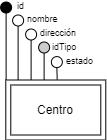
\includegraphics[scale=0.8]{img/diagramas/EER/E-Centro.png}
        \caption{Entidad Centro}
        \label{fig:E-Centro}
    \end{figure}

    \item Ejemplo de entidad (Tabla \ref{table:T-Centro}):

    \begin{table}[H]
    \centering
        \begin{tabular}{ |p{6cm}||p{6cm}|  }
             \hline
                \multicolumn{2}{|c|}{\textbf{Centro}} \\
             \hline
                 \textbf{Atributo} & \textbf{Valor} \\
             \hline
                 id & 1 \\
             \hline
                 nombre & Ciencias \\
             \hline
                 dirección & Campus Rabanales \\
             \hline
                 idTipo & 1 \\
             \hline
                 estado & 1 \\
        \end{tabular}
        \caption{Ejemplo de la entidad \textit{Centro}}
        \label{table:T-Centro}
    \end{table}
\end{itemize}

\subsection{Entidad Junta}
\begin{itemize}
    \item Descripción: este tipo de entidad representa a las juntas registradas en el sistema que tienen vinculación con la Universidad de Córdoba.
    \item Restricciones: es una entidad débil por identificación respecto de la entidad Centro.
    \item Características:
    \begin{itemize}
        \item Nombre de la entidad: Junta.
        \item Tipo: débil.
        \item Atributos heredados: idCentro, heredado de la entidad Centro.
        \item Atributo identificador primario: id.
        \item Atributo identificador alternativo: ninguno.
        \item Número de atributos: 5 (1 heredado y 4 propios).
    \end{itemize}

    \item Atributos propios:
    \begin{itemize}
        \item id
        \begin{itemize}
            \item Definición: código numérico secuencial e incremental que identifica la junta.
            \item Dominio: números enteros mayores que 0.
            \item Tipo: clave primaria.
            \item Opcional: no
            \item Ejemplo: 13
        \end{itemize}

        \item fechaConstitución
        \begin{itemize}
            \item Definición: fecha de creación de la junta.
            \item Dominio: 01/01/1970 hasta 31/12/9999.
            \item Tipo: atributo simple.
            \item Opcional: no
            \item Ejemplo: 10/09/2023
        \end{itemize}

        \item fechaDisolución
        \begin{itemize}
            \item Definición: fecha de disolución de la junta.
            \item Dominio: 01/01/1970 hasta 31/12/9999.
            \item Tipo: atributo simple.
            \item Opcional: sí
            \item Ejemplo: 10/09/2023
        \end{itemize}

        \item estado
        \begin{itemize}
            \item Definición: estado de la junta.
            \item Dominio: 1 (Habilitado), 0 (Deshabilitado).
            \item Tipo: atributo simple.
            \item Opcional: no
            \item Ejemplo: 1
        \end{itemize}
    \end{itemize}

    \item Diagrama (Figura \ref{fig:E-Junta}):

    \begin{figure}[H]
        \centering
        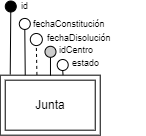
\includegraphics[scale=0.8]{img/diagramas/EER/E-Junta.png}
        \caption{Entidad Junta}
        \label{fig:E-Junta}
    \end{figure}

    \item Ejemplo de entidad (Tabla \ref{table:T-Junta}):

    \begin{table}[H]
    \centering
        \begin{tabular}{ |p{6cm}||p{6cm}|  }
             \hline
                \multicolumn{2}{|c|}{\textbf{Junta}} \\
             \hline
                 \textbf{Atributo} & \textbf{Valor} \\
             \hline
                 id & 1 \\
             \hline
                 fechaConstitución & 10/09/2023 \\
             \hline
                 fechaDisolución & 10/09/2027 \\
             \hline
                 idCentro & 1 \\
             \hline
                 estado & 1 \\
        \end{tabular}
        \caption{Ejemplo de la entidad \textit{Junta}}
        \label{table:T-Junta}
    \end{table}
\end{itemize}

\subsection{Entidad Comisión}
\begin{itemize}
    \item Descripción: este tipo de entidad representa a las comisiones registradas en el sistema que tienen vinculación con la Universidad de Córdoba.
    \item Restricciones: es una entidad débil por identificación respecto de la entidad Junta.
    \item Características:
    \begin{itemize}
        \item Nombre de la entidad: Comisión.
        \item Tipo: débil.
        \item Atributos heredados: idJunta, heredado de la entidad Junta.
        \item Atributo identificador primario: id.
        \item Atributo identificador alternativo: ninguno.
        \item Número de atributos: 7 (1 heredado y 6 propios).
    \end{itemize}

    \item Atributos propios:
    \begin{itemize}
        \item id
        \begin{itemize}
            \item Definición: código numérico secuencial e incremental que identifica la junta.
            \item Dominio: números enteros mayores que 0.
            \item Tipo: clave primaria.
            \item Opcional: no
            \item Ejemplo: 13
        \end{itemize}

         \item nombre
        \begin{itemize}
            \item Definición: nombre que identifica a la comisión.
            \item Dominio: conjunto de 100 caracteres.
            \item Tipo: atributo simple.
            \item Opcional: no
            \item Ejemplo: Asuntos económicos
        \end{itemize}

        \item descripción
        \begin{itemize}
            \item Definición: descripción de la comisión.
            \item Dominio: conjunto de 250 caracteres.
            \item Tipo: atributo simple.
            \item Opcional: no
            \item Ejemplo: Comisión dedicada a abordar todo lo referente a la economía de la comisión.
        \end{itemize}

        \item fechaConstitución
        \begin{itemize}
            \item Definición: fecha de creación de la junta.
            \item Dominio: 01/01/1970 hasta 31/12/9999.
            \item Tipo: atributo simple.
            \item Opcional: no
            \item Ejemplo: 10/09/2023
        \end{itemize}

        \item fechaDisolución
        \begin{itemize}
            \item Definición: fecha de disolución de la junta.
            \item Dominio: 01/01/1970 hasta 31/12/9999.
            \item Tipo: atributo simple.
            \item Opcional: sí
            \item Ejemplo: 10/09/2023
        \end{itemize}

        \item estado
        \begin{itemize}
            \item Definición: estado de la comisión.
            \item Dominio: 1 (Habilitado), 0 (Deshabilitado).
            \item Tipo: atributo simple.
            \item Opcional: no
            \item Ejemplo: 1
        \end{itemize}
    \end{itemize}

    \item Diagrama (Figura \ref{fig:E-Comisión}):

    \begin{figure}[H]
        \centering
        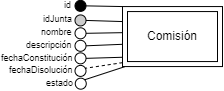
\includegraphics[scale=0.8]{img/diagramas/EER/E-Comisión.png}
        \caption{Entidad Comisión}
        \label{fig:E-Comisión}
    \end{figure}

    \item Ejemplo de entidad (Tabla \ref{table:T-Comisión}):

    \begin{table}[H]
    \centering
        \begin{tabular}{ |p{6cm}||p{6cm}|  }
             \hline
                \multicolumn{2}{|c|}{\textbf{Comisión}} \\
             \hline
                 \textbf{Atributo} & \textbf{Valor} \\
             \hline
                 id & 1 \\
             \hline
                 nombre & Asuntos económicos \\
            \hline
                 descripción & Comisión dedicada a abordar todo lo referente a la economía de la comisión \\
             \hline
                 fechaConstitución & 10/09/2023 \\
             \hline
                 fechaDisolución & 10/09/2027 \\
             \hline
                 idJunta & 1 \\
             \hline
                 estado & 1 \\
        \end{tabular}
        \caption{Ejemplo de la entidad \textit{Comisión}}
        \label{table:T-Comisión}
    \end{table}
\end{itemize}

\subsection{Entidad Convocatoria}
\begin{itemize}
    \item Descripción: este tipo de entidad representa a las convocatorias de comisión y junta registradas en el sistema.
    \item Restricciones: es una entidad débil por identificación respecto de la entidad TipoConvocatoria, la entidad Junta, la entidad Comisión.
    \item Características:
    \begin{itemize}
        \item Nombre de la entidad: Convocatoria.
        \item Tipo: débil.
        \item Atributos heredados: 
        \begin{itemize}
            \item idTipo, heredado de la entidad TipoConvocatoria. 
            \item idJun, heredado de la entidad Junta. 
            \item idCom, heredado de la entidad Comisión.
        \end{itemize}
        \item Atributo identificador primario: id.
        \item Atributo identificador alternativo: ninguno.
        \item Número de atributos: 9 (3 heredados y 6 propios).
    \end{itemize}

    \item Atributos propios:
    \begin{itemize}
        \item id
        \begin{itemize}
            \item Definición: código numérico secuencial e incremental que identifica la junta.
            \item Dominio: números enteros mayores que 0.
            \item Tipo: clave primaria.
            \item Opcional: no
            \item Ejemplo: 13
        \end{itemize}

         \item lugar
        \begin{itemize}
            \item Definición: lugar donde se celebrará la convocatoria.
            \item Dominio: conjunto de 100 caracteres.
            \item Tipo: atributo simple.
            \item Opcional: no
            \item Ejemplo: Rectorado UCO
        \end{itemize}

        \item fecha
        \begin{itemize}
            \item Definición: fecha en la que se celebrará la convocatoria.
            \item Dominio: 01/01/1970 hasta 31/12/9999.
            \item Tipo: atributo simple.
            \item Opcional: no
            \item Ejemplo: 10/09/2023
        \end{itemize}

         \item hora
        \begin{itemize}
            \item Definición: hora en la que se celebrará la convocatoria.
            \item Dominio: 00:00 hasta 23:59.
            \item Tipo: atributo simple.
            \item Opcional: no
            \item Ejemplo: 11:30
        \end{itemize}

        \item actaPDF
        \begin{itemize}
            \item Definición: ruta del documento PDF que contendrá información sobre la convocatoria celebrada.
            \item Dominio: conjunto de 200 caracteres.
            \item Tipo: atributo simple.
            \item Opcional: sí
            \item Ejemplo: /resources/convocatorias/1.pdf
        \end{itemize}

        \item estado
        \begin{itemize}
            \item Definición: estado de la convocatoria.
            \item Dominio: 1 (Habilitado), 0 (Deshabilitado).
            \item Tipo: atributo simple.
            \item Opcional: no
            \item Ejemplo: 1
        \end{itemize}
    \end{itemize}

    \item Diagrama (Figura \ref{fig:E-Convocatoria}):

    \begin{figure}[H]
        \centering
        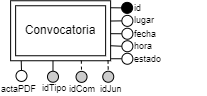
\includegraphics[scale=0.8]{img/diagramas/EER/E-Convocatoria.png}
        \caption{Entidad Convocatoria}
        \label{fig:E-Convocatoria}
    \end{figure}

    \item Ejemplo de entidad (Tabla \ref{table:T-Convocatoria}):

    \begin{table}[H]
    \centering
        \begin{tabular}{ |p{6cm}||p{6cm}|  }
             \hline
                \multicolumn{2}{|c|}{\textbf{Convocatoria}} \\
             \hline
                 \textbf{Atributo} & \textbf{Valor} \\
             \hline
                 id & 1 \\
             \hline
                 lugar & Rectorado UCO \\
            \hline
                 fecha & 10/09/2023 \\
             \hline
                 hora & 11:30 \\
             \hline
                 idTipo & 1 \\
             \hline
                 idJun & 1 \\
             \hline
                idCom &  \\
             \hline
                 estado & 1 \\
        \end{tabular}
        \caption{Ejemplo de la entidad \textit{Convocatoria}}
        \label{table:T-Convocatoria}
    \end{table}
\end{itemize}

\subsection{Entidad MiembroGobierno}
\begin{itemize}
    \item Descripción: este tipo de entidad representa a los miembros del equipo de gobierno de cada centro registrados en el sistema que tienen vinculación con la Universidad de Córdoba.
    \item Restricciones: es una entidad débil por identificación respecto de la entidad Usuario, la entidad Centro y la entidad TipoRepresentaciónGobierno.
    \item Características:
    \begin{itemize}
        \item Nombre de la entidad: MiembroGobierno.
        \item Tipo: débil.
        \item Atributos heredados: 
        \begin{itemize}
            \item idUsuario, heredado de la entidad Usuario.
            \item idCentro, heredado de la entidad Centro.
            \item idRepresentacion, heredado de la entidad TipoRepresentaciónGobierno.
        \end{itemize} 
        \item Atributo identificador primario: id.
        \item Atributo identificador alternativo: ninguno.
        \item Número de atributos: 6 (3 heredados y 3 propios).
    \end{itemize}

    \item Atributos propios:
    \begin{itemize}
        \item id
        \begin{itemize}
            \item Definición: código numérico secuencial e incremental que identifica la junta.
            \item Dominio: números enteros mayores que 0.
            \item Tipo: clave primaria.
            \item Opcional: no
            \item Ejemplo: 13
        \end{itemize}

        \item fechaTomaPosesión
        \begin{itemize}
            \item Definición: fecha de toma de posesión del miembro de gobierno.
            \item Dominio: 01/01/1970 hasta 31/12/9999.
            \item Tipo: atributo simple.
            \item Opcional: no
            \item Ejemplo: 10/09/2023
        \end{itemize}

        \item fechaCese
        \begin{itemize}
            \item Definición: fecha de cese del miembro de gobierno.
            \item Dominio: 01/01/1970 hasta 31/12/9999.
            \item Tipo: atributo simple.
            \item Opcional: sí
            \item Ejemplo: 10/09/2023
        \end{itemize}

        \item estado
        \begin{itemize}
            \item Definición: estado del miembro del gobierno.
            \item Dominio: 1 (Habilitado), 0 (Deshabilitado).
            \item Tipo: atributo simple.
            \item Opcional: no
            \item Ejemplo: 1
        \end{itemize}
    \end{itemize}

    \item Diagrama (Figura \ref{fig:E-MiembroGobierno}):

    \begin{figure}[H]
        \centering
        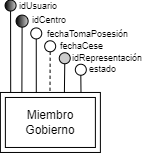
\includegraphics[scale=0.8]{img/diagramas/EER/E-MiembroGobierno.png}
        \caption{Entidad MiembroGobierno}
        \label{fig:E-MiembroGobierno}
    \end{figure}

    \item Ejemplo de entidad (Tabla \ref{table:T-MiembroGobierno}):

    \begin{table}[H]
    \centering
        \begin{tabular}{ |p{6cm}||p{6cm}|  }
             \hline
                \multicolumn{2}{|c|}{\textbf{MiembroGobierno}} \\
             \hline
                 \textbf{Atributo} & \textbf{Valor} \\
             \hline
                 id & 1 \\
             \hline
                 fechaTomaPosesión & 10/09/2023 \\
             \hline
                 fechaCese & 10/09/2027 \\
             \hline
                 idUsuario & 1 \\
             \hline
                 idCentro & 1 \\
            \hline
                 idRepresentación & 1 \\
             \hline
                 estado & 1 \\
        \end{tabular}
        \caption{Ejemplo de la entidad \textit{MiembroGobierno}}
        \label{table:T-MiembroGobierno}
    \end{table}
\end{itemize}

\subsection{Entidad MiembroJunta}
\begin{itemize}
    \item Descripción: este tipo de entidad representa a los miembros de la junta de cada centro registrados en el sistema que tienen vinculación con la Universidad de Córdoba.
    \item Restricciones: es una entidad débil por identificación respecto de la entidad Usuario, la entidad Junta y la entidad TipoRepresentaciónGeneral.
    \item Características:
    \begin{itemize}
        \item Nombre de la entidad: MiembroJunta.
        \item Tipo: débil.
        \item Atributos heredados: 
        \begin{itemize}
            \item idUsuario, heredado de la entidad Usuario.
            \item idJunta, heredado de la entidad Junta.
            \item idRepresentacion, heredado de la entidad TipoRepresentaciónGeneral.
        \end{itemize} 
        \item Atributo identificador primario: id.
        \item Atributo identificador alternativo: ninguno.
        \item Número de atributos: 6 (3 heredados y 3 propios).
    \end{itemize}

    \item Atributos propios:
    \begin{itemize}
        \item id
        \begin{itemize}
            \item Definición: código numérico secuencial e incremental que identifica la junta.
            \item Dominio: números enteros mayores que 0.
            \item Tipo: clave primaria.
            \item Opcional: no
            \item Ejemplo: 13
        \end{itemize}

        \item fechaTomaPosesión
        \begin{itemize}
            \item Definición: fecha de toma de posesión del miembro de gobierno.
            \item Dominio: 01/01/1970 hasta 31/12/9999.
            \item Tipo: atributo simple.
            \item Opcional: no
            \item Ejemplo: 10/09/2023
        \end{itemize}

        \item fechaCese
        \begin{itemize}
            \item Definición: fecha de cese del miembro de gobierno.
            \item Dominio: 01/01/1970 hasta 31/12/9999.
            \item Tipo: atributo simple.
            \item Opcional: sí
            \item Ejemplo: 10/09/2023
        \end{itemize}

        \item estado
        \begin{itemize}
            \item Definición: estado del miembro de la junta.
            \item Dominio: 1 (Habilitado), 0 (Deshabilitado).
            \item Tipo: atributo simple.
            \item Opcional: no
            \item Ejemplo: 1
        \end{itemize}
    \end{itemize}

    \item Diagrama (Figura \ref{fig:E-MiembroJunta}):

    \begin{figure}[H]
        \centering
        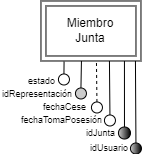
\includegraphics[scale=0.8]{img/diagramas/EER/E-MiembroJunta.png}
        \caption{Entidad MiembroJunta}
        \label{fig:E-MiembroJunta}
    \end{figure}

    \item Ejemplo de entidad (Tabla \ref{table:T-MiembroJunta}):

    \begin{table}[H]
    \centering
        \begin{tabular}{ |p{6cm}||p{6cm}|  }
             \hline
                \multicolumn{2}{|c|}{\textbf{MiembroJunta}} \\
             \hline
                 \textbf{Atributo} & \textbf{Valor} \\
             \hline
                 id & 1 \\
             \hline
                 fechaTomaPosesión & 10/09/2023 \\
             \hline
                 fechaCese & 10/09/2027 \\
             \hline
                 idUsuario & 1 \\
             \hline
                 idJunta & 1 \\
            \hline
                 idRepresentación & 1 \\
             \hline
                 estado & 1 \\
        \end{tabular}
        \caption{Ejemplo de la entidad \textit{MiembroJunta}}
        \label{table:T-MiembroJunta}
    \end{table}
\end{itemize}

\subsection{Entidad MiembroComisión}
\begin{itemize}
    \item Descripción: este tipo de entidad representa a los miembros de la comisión de cada junta de cada centro registrados en el sistema que tienen vinculación con la Universidad de Córdoba.
    \item Restricciones: es una entidad débil por identificación respecto de la entidad Usuario, la entidad Comsii¡sión y la entidad TipoRepresentaciónGeneral.
    \item Características:
    \begin{itemize}
        \item Nombre de la entidad: MiembroComisión.
        \item Tipo: débil.
        \item Atributos heredados: 
        \begin{itemize}
            \item idUsuario, heredado de la entidad Usuario.
            \item idComisión, heredado de la entidad Comisión.
            \item idRepresentacion, heredado de la entidad TipoRepresentaciónGeneral.
        \end{itemize} 
        \item Atributo identificador primario: id.
        \item Atributo identificador alternativo: ninguno.
        \item Número de atributos: 6 (3 heredados y 3 propios).
    \end{itemize}

    \item Atributos propios:
    \begin{itemize}
        \item id
        \begin{itemize}
            \item Definición: código numérico secuencial e incremental que identifica la junta.
            \item Dominio: números enteros mayores que 0.
            \item Tipo: clave primaria.
            \item Opcional: no
            \item Ejemplo: 13
        \end{itemize}

        \item fechaTomaPosesión
        \begin{itemize}
            \item Definición: fecha de toma de posesión del miembro de gobierno.
            \item Dominio: 01/01/1970 hasta 31/12/9999.
            \item Tipo: atributo simple.
            \item Opcional: no
            \item Ejemplo: 10/09/2023
        \end{itemize}

        \item fechaCese
        \begin{itemize}
            \item Definición: fecha de cese del miembro de gobierno.
            \item Dominio: 01/01/1970 hasta 31/12/9999.
            \item Tipo: atributo simple.
            \item Opcional: sí
            \item Ejemplo: 10/09/2023
        \end{itemize}

        \item estado
        \begin{itemize}
            \item Definición: estado del miembro de la comisión.
            \item Dominio: 1 (Habilitado), 0 (Deshabilitado).
            \item Tipo: atributo simple.
            \item Opcional: no
            \item Ejemplo: 1
        \end{itemize}
    \end{itemize}

    \item Diagrama (Figura \ref{fig:E-MiembroComisión}):

    \begin{figure}[H]
        \centering
        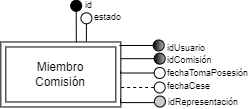
\includegraphics[scale=0.8]{img/diagramas/EER/E-MiembroComisión.png}
        \caption{Entidad MiembroComisión}
        \label{fig:E-MiembroComisión}
    \end{figure}

    \item Ejemplo de entidad (Tabla \ref{table:T-MiembroComisión}):

    \begin{table}[H]
    \centering
        \begin{tabular}{ |p{6cm}||p{6cm}|  }
             \hline
                \multicolumn{2}{|c|}{\textbf{MiembroComisión}} \\
             \hline
                 \textbf{Atributo} & \textbf{Valor} \\
             \hline
                 id & 1 \\
             \hline
                 fechaTomaPosesión & 10/09/2023 \\
             \hline
                 fechaCese & 10/09/2027 \\
             \hline
                 idUsuario & 1 \\
             \hline
                 idComisión & 1 \\
            \hline
                 idRepresentación & 1 \\
             \hline
                 estado & 1 \\
        \end{tabular}
        \caption{Ejemplo de la entidad \textit{MiembroComisión}}
        \label{table:T-MiembroComisión}
    \end{table}
\end{itemize}


\section{Tipos de interrelación} \label{sec:relaciones}
En esta sección se identificarán y describirán las interrelaciones entre los tipos de entidad descritos en la sección 7.2.

Las interrelaciones pueden ser de tipo débil o fuerte.

\begin{itemize}
    \item Un tipo de Interrelación Fuerte es aquella que representa la relación existente entre dos tipos de entidad fuertes.

    \item Un tipo de Interrelación Débil es aquella que representa la relación entre un tipo de entidad débil y otro fuerte o entre dos tipos de entidad débiles.
\end{itemize}

De acuerdo con la notación del modelo E-R, una interrelación se representa mediante un rombo del que parten flechas hacia los tipos de entidad que forman parte de la relación. Cada tipo de entidad interviene en la interrelación con una determinada cardinalidad, que indica el número mínimo y máximo de instancias de cada tipo de entidad que pueden participar en la interrelación. Se representa por dos valores entre paréntesis (mínimo y máximo). Las posibles cardinalidades son: (0,1), (1,1),(0,n),(1,n),(m,n). Estas cardinalidades determinan el tipo de interrelación que se está definiendo, que puede ser:

\begin{itemize}
    \item \textbf{1:1} Uno a uno. Cuando los dos tipos de entidad participan con una cardinalidad máxima de 1.
    \item \textbf{1:N o N:1} Uno a muchos, o muchos a uno. Cuando uno de los tipos de entidad participa con una cardinalidad máxima de 1 y el otro con una cardinalidad máxima de n.
    \item \textbf{N:N} Muchos a muchos. Cuando ambos tipos de entidad participan una cardinalidad máxima de n.
\end{itemize}

Para cada una de las interrelaciones que se han identificado en la definición del problema, se indicará la siguiente información:

\begin{itemize}
    \item \textbf{Nombre}. Nombre del tipo de interrelación.
    \item \textbf{Descripción}. Definición del tipo de interrelación y de los tipos de entidad que participan en ella.
    \item \textbf{Tipo}. Indicación de si se trata de un tipo de interrelación débil o fuerte identificando los tipos de debilidad en su caso.
    \item \textbf{Cardinalidad}. Indicación de la cardinalidad del tipo de interrelación y cardinalidades mínima y máxima de los tipos de entidad intervinientes.
    \item \textbf{Atributos}. Indicación del número y descripción de los atributos del tipo de interrelación, en su caso.
    \item \textbf{Diagrama}. Representación gráfica del tipo de interrelación, de acuerdo con la notación E-R.
    \item \textbf{Ejemplo}. Valores de muestra.
\end{itemize}

Se han identificado las interrelaciones que se indican a continuación y que se describirán en las siguientes subsecciones:

\begin{itemize}
    \item Tipo de Interrelación: TipoCentro - Centro.
    \item Tipo de Interrelación: TipoRepresentaciónGobierno - MiembroGobierno.
    \item Tipo de Interrelación: TipoRepresentaciónGeneral - MiembroJunta.
    \item Tipo de Interrelación: TipoRepresentaciónGeneral - MiembroComisión.
    \item Tipo de Interrelación: TipoConvocatoria - Convocatoria.
    \item Tipo de Interrelación: Centro - MiembroGobierno.
    \item Tipo de Interrelación: Centro - Junta.
    \item Tipo de Interrelación: Junta - MiembroJunta.
    \item Tipo de Interrelación: Junta - Comisión.
    \item Tipo de Interrelación: Junta - Convocatoria.
    \item Tipo de Interrelación: Comisión - MiembroComisión.
    \item Tipo de Interrelación: Comisión - Convocatoria.
    \item Tipo de Interrelación: Usuario - MiembroGobierno.
    \item Tipo de Interrelación: Usuario - MiembroJunta.
    \item Tipo de Interrelación: Usuario - MiembroComisión.
\end{itemize}

\subsection{Interrelación: TipoCentro - Centro}
\begin{itemize}
    \item \textbf{Nombre}: TipCt-Ct.
    \item \textbf{Descripción}: esta interrelación muestra que un tipo de centro puede corresponder a cero, uno o más centros, pero un centro solamente tiene un tipo de centro.
    \item \textbf{Tipo}: la entidad Centro presenta una debilidad por identificación respecto de la entidad Tipo Centro.
    \item \textbf{Cardinalidad}. 1:N
    \begin{itemize}
        \item Cardinalidad de TipoCentro (0,n): un tipo de centro puede tener asociadas 0, 1 o varios centros.
        \item Cardinalidad de Centro (1,1): un centro solamente está asociado a un tipo de centro.
    \end{itemize}
    \item \textbf{Atributos}: ninguno
    \item \textbf{Diagrama} (Figura \ref{fig:I-TipCt-Ct}) 
    \begin{figure}[H]
        \centering
        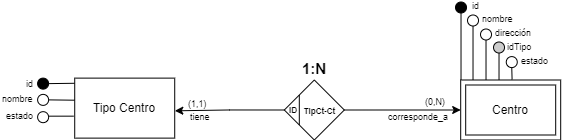
\includegraphics[scale=0.7]{img/diagramas/EER/I-TipCt-Ct.png}
        \caption{Interrelación: TipoCentro - Centro}
        \label{fig:I-TipCt-Ct}
    \end{figure}
    
    \item \textbf{Ejemplo} (Tabla \ref{table:I-TipCt-Ct}).

    \begin{table}[H]
    \centering
        \begin{tabular}{ | c | c | c |  }
             \hline
                 \textbf{Entidad} & \textbf{Atributo} & \textbf{Ejemplo}\\       
             \hline
                 \textbf{Tipo Centro}  & \underline{id} & 1\\
                  & nombre & Facultad\\
                  & estado & 1\\
             \hline
                 \textbf{Centro}  & \underline{id} & 1\\
                  & nombre & Ciencias\\
                  & dirección & Campus de Rabanales\\
                  & idTipo & 1\\
                  & estado & 1\\
        \end{tabular}
        \caption{Ejemplo de la interrelación \textit{TipoCentro - Centro}}
        \label{table:I-TipCt-Ct}
    \end{table}

\end{itemize}

\subsection{Interrelación: TipoRepresentaciónGobierno - MiembroGobierno }
\begin{itemize}
    \item \textbf{Nombre}: TipGob-MiGob.
    \item \textbf{Descripción}: esta interrelación muestra que un tipo de representación de gobierno puede corresponder a cero, uno o más miembros de gobierno, pero un miembro de gobierno solamente tiene un tipo de representación de gobierno.
    \item \textbf{Tipo}: la entidad Miembro Gobierno presenta una debilidad por identificación respecto de la entidad Tipo Representación Gobierno.
    \item \textbf{Cardinalidad}. 1:N
    \begin{itemize}
        \item Cardinalidad de TipoRepresentaciónGobierno (0,n): un tipo de representación gobierno puede tener asociadas 0, 1 o varios miembros de gobierno.
        \item Cardinalidad de MiembroGobierno (1,1): un miembro de gobierno solamente está asociado a un tipo de representación de gobierno.
    \end{itemize}
    \item \textbf{Atributos}: ninguno
    \item \textbf{Diagrama} (Figura \ref{fig:I-TipGob-MiGob}) 
    \begin{figure}[H]
        \centering
        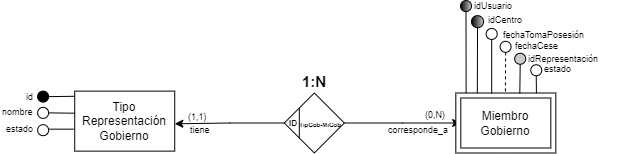
\includegraphics[scale=0.7]{img/diagramas/EER/I-TipGob-MiGob.png}
        \caption{Interrelación: TipoRepresentaciónGobierno - MiembroGobierno}
        \label{fig:I-TipGob-MiGob}
    \end{figure}
    
    \item \textbf{Ejemplo} (Tabla \ref{table:I-TipGob-MiGob}).

    \begin{table}[H]
    \centering
        \begin{tabular}{ | c | c | c |  }
             \hline
                 \textbf{Entidad} & \textbf{Atributo} & \textbf{Ejemplo}\\       
             \hline
                 \textbf{Tipo Representación Gobierno}  & \underline{id} & 1\\
                  & nombre & Director\\
                  & estado & 1\\
             \hline
                 \textbf{Miembro Gobierno}  & \underline{id} & 1\\
                  & idUsuario & 1\\
                  & idCentro & 1\\
                  & idRepresentación & 1\\
                  & fechaTomaPosesión & 10/09/2023\\
                  & fechaCese & null\\
                  & estado & 1\\
        \end{tabular}
        \caption{Ejemplo de la interrelación \textit{TipoRepresentaciónGobierno - MiembroGobierno}}
        \label{table:I-TipGob-MiGob}
    \end{table}
\end{itemize}

\subsection{Interrelación: TipoRepresentaciónGeneral - MiembroJunta}
\begin{itemize}
    \item \textbf{Nombre}: TipRG-MiJu.
    \item \textbf{Descripción}: esta interrelación muestra que un tipo de representación general puede corresponder a cero, uno o más miembros de junta, pero un miembro de junta solamente tiene un tipo de representación general.
    \item \textbf{Tipo}: la entidad Miembro Junta presenta una debilidad por identificación respecto de la entidad Tipo Representación General.
    \item \textbf{Cardinalidad}. 1:N
    \begin{itemize}
        \item Cardinalidad de TipoRepresentaciónGeneral (0,n): un tipo de representación general puede tener asociadas 0, 1 o varios miembros de junta.
        \item Cardinalidad de MiembroJunta (1,1): un miembro de junta solamente está asociado a un tipo de representación general.
    \end{itemize}
    \item \textbf{Atributos}: ninguno
    \item \textbf{Diagrama} (Figura \ref{fig:I-TipRG-MiJu}) 
    \begin{figure}[H]
        \centering
        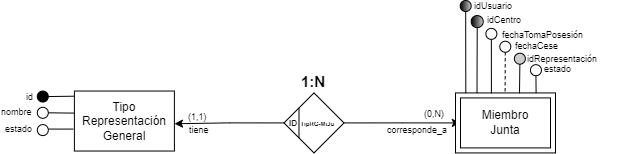
\includegraphics[scale=0.7]{img/diagramas/EER/I-TipRG-MiJu.png}
        \caption{Interrelación: TipoRepresentaciónGeneral - MiembroJunta}
        \label{fig:I-TipRG-MiJu}
    \end{figure}
    
    \item \textbf{Ejemplo} (Tabla \ref{table:I-TipRG-MiJu}).

    \begin{table}[H]
    \centering
        \begin{tabular}{ | c | c | c |  }
             \hline
                 \textbf{Entidad} & \textbf{Atributo} & \textbf{Ejemplo}\\       
             \hline
                 \textbf{Tipo Representación General}  & \underline{id} & 1\\
                  & nombre & Profesorado vinculación permanente\\
                  & estado & 1\\
             \hline
                 \textbf{Miembro Junta}  & \underline{id} & 1\\
                  & idUsuario & 1\\
                  & idJunta & 1\\
                  & idRepresentación & 1\\
                  & fechaTomaPosesión & 10/09/2023\\
                  & fechaCese & null\\
                  & estado & 1\\
        \end{tabular}
        \caption{Ejemplo de la interrelación \textit{TipoRepresentaciónGeneral - MiembroJunta}}
        \label{table:I-TipRG-MiJu}
    \end{table}
\end{itemize}

\subsection{Interrelación: TipoRepresentaciónGeneral - MiembroComisión}
\begin{itemize}
    \item \textbf{Nombre}: TipRG-MiCom.
    \item \textbf{Descripción}: esta interrelación muestra que un tipo de representación general puede corresponder a cero, uno o más miembros de comisión, pero un miembro de comisión solamente tiene un tipo de representación general.
    \item \textbf{Tipo}: la entidad Miembro Comisión presenta una debilidad por identificación respecto de la entidad Tipo Representación General.
    \item \textbf{Cardinalidad}. 1:N
    \begin{itemize}
        \item Cardinalidad de TipoRepresentaciónGeneral (0,n): un tipo de representación general puede tener asociadas 0, 1 o varios miembros de comisión.
        \item Cardinalidad de MiembroComisión (1,1): un miembro de comisión solamente está asociado a un tipo de representación general.
    \end{itemize}
    \item \textbf{Atributos}: ninguno
    \item \textbf{Diagrama} (Figura \ref{fig:I-TipRG-MiCom}) 
    \begin{figure}[H]
        \centering
        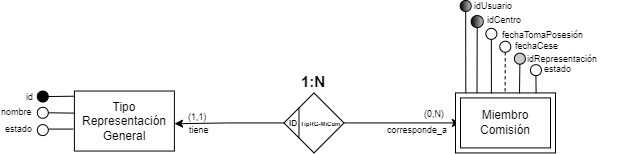
\includegraphics[scale=0.7]{img/diagramas/EER/I-TipRG-MiCom.png}
        \caption{Interrelación: TipoRepresentaciónGeneral - MiembroComisión}
        \label{fig:I-TipRG-MiCom}
    \end{figure}
    
    \item \textbf{Ejemplo} (Tabla \ref{table:I-TipRG-MiCom}).

    \begin{table}[H]
    \centering
        \begin{tabular}{ | c | c | c |  }
             \hline
                 \textbf{Entidad} & \textbf{Atributo} & \textbf{Ejemplo}\\       
             \hline
                 \textbf{Tipo Representación General}  & \underline{id} & 2\\
                  & nombre & PAS\\
                  & estado & 1\\
             \hline
                 \textbf{Miembro Comisión}  & \underline{id} & 1\\
                  & idUsuario & 1\\
                  & idComisión & 1\\
                  & idRepresentación & 2\\
                  & fechaTomaPosesión & 10/09/2023\\
                  & fechaCese & null\\
                  & estado & 1\\
        \end{tabular}
        \caption{Ejemplo de la interrelación \textit{TipoRepresentaciónGeneral - MiembroComisión}}
        \label{table:I-TipRG-MiCom}
    \end{table}
\end{itemize}

\subsection{Interrelación: TipoConvocatoria - Convocatoria}
\begin{itemize}
    \item \textbf{Nombre}: TipConv-Conv.
    \item \textbf{Descripción}: esta interrelación muestra que un tipo de convocatoria puede corresponder a cero, uno o más convocatorias, pero una convocatoria solamente tiene un tipo de convocatoria.
    \item \textbf{Tipo}: la entidad Convocatoria presenta una debilidad por identificación respecto de la entidad Tipo Convocatoria.
    \item \textbf{Cardinalidad}. 1:N
    \begin{itemize}
        \item Cardinalidad de Tipo Convocatoria (0,n): un tipo de convocatoria puede tener asociadas 0, 1 o varias convocatorias.
        \item Cardinalidad de Convocatoria (1,1): una convocatoria solamente está asociada a un tipo de convocatoria.
    \end{itemize}
    \item \textbf{Atributos}: ninguno
    \item \textbf{Diagrama} (Figura \ref{fig:I-TipConv-Conv}) 
    \begin{figure}[H]
        \centering
        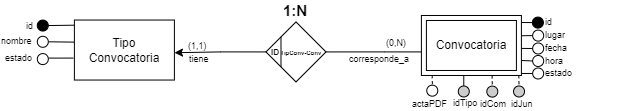
\includegraphics[scale=0.7]{img/diagramas/EER/I-TipConv-Conv.png}
        \caption{Interrelación: TipoConvocatoria - Convocatoria}
        \label{fig:I-TipConv-Conv}
    \end{figure}
    
    \item \textbf{Ejemplo} (Tabla \ref{table:I-TipConv-Conv}).

    \begin{table}[H]
    \centering
        \begin{tabular}{ | c | c | c |  }
             \hline
                 \textbf{Entidad} & \textbf{Atributo} & \textbf{Ejemplo}\\       
             \hline
                 \textbf{Tipo Convocvatoria}  & \underline{id} & 1\\
                  & nombre & Ordinaria\\
                  & estado & 1\\
             \hline
                 \textbf{Convocatoria}  & \underline{id} & 1\\
                  & lugar & Rectorado\\
                  & fecha & 23/09/2023\\
                  & hora & 11:30\\
                  & idTipo & 1\\
                  & idComision & null\\
                  & idJunta & 1\\
                  & acta & /resources/actas/1.pdf \\
                  & estado & 1\\
        \end{tabular}
        \caption{Ejemplo de la interrelación \textit{TipoConvocatoria - Convocatoria}}
        \label{table:I-TipConv-Conv}
    \end{table}
\end{itemize}

\subsection{Interrelación: Centro - MiembroGobierno}
\begin{itemize}
    \item \textbf{Nombre}: Ct-MiGob.
    \item \textbf{Descripción}: esta interrelación muestra que un centro puede ser representado por uno o más miembros de gobierno, pero un miembro de gobierno solamente representa un centro.
    \item \textbf{Tipo}: la entidad MiembroGobierno presenta una debilidad por identificación respecto de la entidad Centro.
    \item \textbf{Cardinalidad}. 1:N
    \begin{itemize}
        \item Cardinalidad de Centro (1,n): un centro puede tener asociados 1 o varias miembros de gobierno.
        \item Cardinalidad de MiembroGobierno (1,1): un miembro de gobierno solamente está asociado a un centro.
    \end{itemize}
    \item \textbf{Atributos}: ninguno
    \item \textbf{Diagrama} (Figura \ref{fig:I-Ct-MiGob}) 
    \begin{figure}[H]
        \centering
        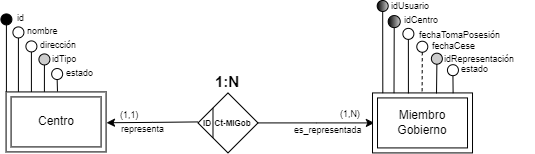
\includegraphics[scale=0.7]{img/diagramas/EER/I-Ct-MiGob.png}
        \caption{Interrelación: Centro - MiembroGobierno}
        \label{fig:I-Ct-MiGob}
    \end{figure}
    
    \item \textbf{Ejemplo} (Tabla \ref{table:I-Ct-MiGob}).

    \begin{table}[H]
    \centering
        \begin{tabular}{ | c | c | c |  }
             \hline
                 \textbf{Entidad} & \textbf{Atributo} & \textbf{Ejemplo}\\       
             \hline
                 \textbf{Centro}  & \underline{id} & 1\\
                  & nombre & Ciencias\\
                  & dirección & Campus de Rabanales\\
                  & idTipo & 1\\
                  & estado & 1\\
             \hline
                 \textbf{Miembro Gobierno}  & \underline{id} & 1\\
                  & idUsuario & 1\\
                  & idCentro & 1\\
                  & idRepresentación & 1\\
                  & fechaTomaPosesión & 10/09/2023\\
                  & fechaCese & null\\
                  & estado & 1\\
        \end{tabular}
        \caption{Ejemplo de la interrelación \textit{Centro - MiembroGobierno}}
        \label{table:I-Ct-MiGob}
    \end{table}
\end{itemize}

\subsection{Interrelación: Centro - Junta}
\begin{itemize}
    \item \textbf{Nombre}: Ct-Ju.
    \item \textbf{Descripción}: esta interrelación muestra que un centro puede ser coordinado por cero, uno o más juntas, pero una junta solamente coordina un centro.
    \item \textbf{Tipo}: la entidad Junta presenta una debilidad por identificación respecto de la entidad Centro.
    \item \textbf{Cardinalidad}. 1:N
    \begin{itemize}
        \item Cardinalidad de Centro (0,n): un centro puede tener asociados 0, 1 o varias juntas.
        \item Cardinalidad de Junta (1,1): una junta solamente está asociada a un centro.
    \end{itemize}
    \item \textbf{Atributos}: ninguno
    \item \textbf{Diagrama} (Figura \ref{fig:I-Ct-Ju}) 
    \begin{figure}[H]
        \centering
        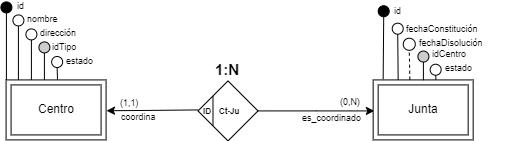
\includegraphics[scale=0.7]{img/diagramas/EER/I-Ct-Ju}
        \caption{Interrelación: Centro - Junta}
        \label{fig:I-Ct-Ju}
    \end{figure}
    
    \item \textbf{Ejemplo} (Tabla \ref{table:I-Ct-Ju}).

    \begin{table}[H]
    \centering
        \begin{tabular}{ | c | c | c |  }
             \hline
                 \textbf{Entidad} & \textbf{Atributo} & \textbf{Ejemplo}\\       
             \hline
                 \textbf{Centro}  & \underline{id} & 1\\
                  & nombre & Ciencias\\
                  & dirección & Campus de Rabanales\\
                  & idTipo & 1\\
                  & estado & 1\\
             \hline
                 \textbf{Junta}  & \underline{id} & 1\\
                  & idCentro & 1\\
                  & fechaConstitución & 10/09/2023\\
                  & fechaDisolución & null\\
                  & estado & 1\\
        \end{tabular}
        \caption{Ejemplo de la interrelación \textit{Centro - Junta}}
        \label{table:I-Ct-Ju}
    \end{table}
\end{itemize}

\subsection{Interrelación: Junta - MiembroJunta}
\begin{itemize}
    \item \textbf{Nombre}: Ju-MiJu.
    \item \textbf{Descripción}: esta interrelación muestra que una junta puede ser representada por cero, uno o más miembros de junta, pero un miembro de junta solamente representa una junta.
    \item \textbf{Tipo}: la entidad MiembroJunta presenta una debilidad por identificación respecto de la entidad Junta.
    \item \textbf{Cardinalidad}. 1:N
    \begin{itemize}
        \item Cardinalidad de Junta (0,n): una junta puede tener asociados 0, 1 o varios miembros de junta.
        \item Cardinalidad de MiembroJunta (1,1): un miembro de junta solamente está asociado a una junta.
    \end{itemize}
    \item \textbf{Atributos}: ninguno
    \item \textbf{Diagrama} (Figura \ref{fig:I-Ju-MiJu}) 
    \begin{figure}[H]
        \centering
        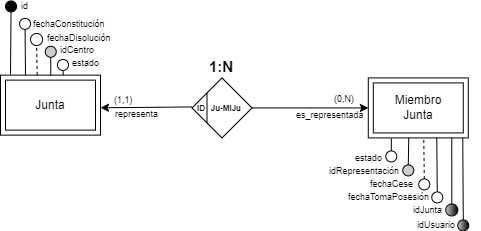
\includegraphics[scale=0.7]{img/diagramas/EER/I-Ju-MiJu}
        \caption{Interrelación: Junta - MiembroJunta}
        \label{fig:I-Ju-MiJu}
    \end{figure}
    
    \item \textbf{Ejemplo} (Tabla \ref{table:I-Ju-MiJu}).

    \begin{table}[H]
    \centering
        \begin{tabular}{ | c | c | c |  }
             \hline
                 \textbf{Entidad} & \textbf{Atributo} & \textbf{Ejemplo}\\       
             \hline
                 \textbf{Junta}  & \underline{id} & 1\\
                  & idCentro & 1\\
                  & fechaConstitución & 10/09/2023\\
                  & fechaDisolución & null\\
                  & estado & 1\\
              \hline
                 \textbf{Miembro Junta}  & \underline{id} & 1\\
                  & idUsuario & 1\\
                  & idJunta & 1\\
                  & idRepresentación & 1\\
                  & fechaTomaPosesión & 10/09/2023\\
                  & fechaCese & null\\
                  & estado & 1\\
        \end{tabular}
        \caption{Ejemplo de la interrelación \textit{Junta - MiembroJunta}}
        \label{table:I-Ju-MiJu}
    \end{table}
\end{itemize}

\subsection{Interrelación: Junta - Comisión}
\begin{itemize}
    \item \textbf{Nombre}: Ju-Com.
    \item \textbf{Descripción}: esta interrelación muestra que una junta puede gestionar cero, uno o más comisiones, pero una comisión solamente puede ser gestionada por una junta.
    \item \textbf{Tipo}: la entidad Comisión presenta una debilidad por identificación respecto de la entidad Junta.
    \item \textbf{Cardinalidad}. 1:N
    \begin{itemize}
        \item Cardinalidad de Junta (0,n): una junta puede tener asociados 0, 1 o varias comisiones.
        \item Cardinalidad de Comisión (1,1): una comisión solamente está asociado a una junta.
    \end{itemize}
    \item \textbf{Atributos}: ninguno
    \item \textbf{Diagrama} (Figura \ref{fig:I-Ju-Com}) 
    \begin{figure}[H]
        \centering
        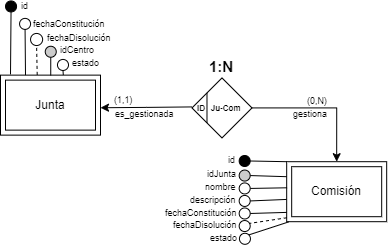
\includegraphics[scale=0.7]{img/diagramas/EER/I-Ju-Com}
        \caption{Interrelación: Junta - Comisión}
        \label{fig:I-Ju-Com}
    \end{figure}
    
    \item \textbf{Ejemplo} (Tabla \ref{table:I-Ju-Com}).

    \begin{table}[H]
    \centering
        \begin{tabular}{ | c | c | c |  }
             \hline
                 \textbf{Entidad} & \textbf{Atributo} & \textbf{Ejemplo}\\       
             \hline
                 \textbf{Junta}  & \underline{id} & 1\\
                  & idCentro & 1\\
                  & fechaConstitución & 10/09/2023\\
                  & fechaDisolución & null\\
                  & estado & 1\\
              \hline
                 \textbf{Comisión}  & \underline{id} & 1\\
                  & id & 1\\
                  & idJunta & 1\\
                  & nombre & Asuntos económicos\\
                  & descripción & Economía de la comisión\\
                  & fechaConstitución & 10/09/2023\\
                  & fechaDisolución & null\\
                  & estado & 1\\
        \end{tabular}
        \caption{Ejemplo de la interrelación \textit{Junta - Comisión}}
        \label{table:I-Ju-Com}
    \end{table}
\end{itemize}

\subsection{Interrelación: Junta - Convocatoria}
\begin{itemize}
    \item \textbf{Nombre}: Ju-Conv.
    \item \textbf{Descripción}: esta interrelación muestra que una junta puede gestionar cero, uno o más convocatorias, pero una convocatoria solamente puede ser gestionada por una junta.
    \item \textbf{Tipo}: la entidad Convocatoria presenta una debilidad por identificación respecto de la entidad Junta.
    \item \textbf{Cardinalidad}. 1:N
    \begin{itemize}
        \item Cardinalidad de Junta (0,n): una junta puede tener asociados 0, 1 o varias convocatorias.
        \item Cardinalidad de Convocatoria (1,1): una convocatoria solamente está asociado a una junta.
    \end{itemize}
    \item \textbf{Atributos}: ninguno
    \item \textbf{Diagrama} (Figura \ref{fig:I-Ju-Conv}) 
    \begin{figure}[H]
        \centering
        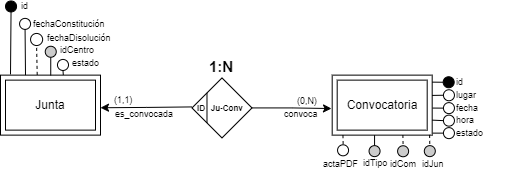
\includegraphics[scale=0.7]{img/diagramas/EER/I-Ju-Conv}
        \caption{Interrelación: Junta - Convocatoria}
        \label{fig:I-Ju-Conv}
    \end{figure}
    
    \item \textbf{Ejemplo} (Tabla \ref{table:I-Ju-Conv}).

    \begin{table}[H]
    \centering
        \begin{tabular}{ | c | c | c |  }
             \hline
                 \textbf{Entidad} & \textbf{Atributo} & \textbf{Ejemplo}\\       
             \hline
                 \textbf{Junta}  & \underline{id} & 1\\
                  & idCentro & 1\\
                  & fechaConstitución & 10/09/2023\\
                  & fechaDisolución & null\\
                  & estado & 1\\
              \hline
                  \textbf{Convocatoria}  & \underline{id} & 1\\
                  & lugar & Rectorado\\
                  & fecha & 23/09/2023\\
                  & hora & 11:30\\
                  & idTipo & 1\\
                  & idComision & null\\
                  & idJunta & 1\\
                  & acta & /resources/actas/1.pdf \\
                  & estado & 1\\
        \end{tabular}
        \caption{Ejemplo de la interrelación \textit{Junta - Convocatoria}}
        \label{table:I-Ju-Conv}
    \end{table}
\end{itemize}

\subsection{Interrelación: Comisión - MiembroComisión}
\begin{itemize}
    \item \textbf{Nombre}: Com-MiCom.
    \item \textbf{Descripción}: esta interrelación muestra que una comisión puede ser representada por cero, uno o más miembros de comisión, pero un miembro de comisión solamente representa una comisión.
    \item \textbf{Tipo}: la entidad MiembroComisión presenta una debilidad por identificación respecto de la entidad Comisión.
    \item \textbf{Cardinalidad}. 1:N
    \begin{itemize}
        \item Cardinalidad de Comisión (0,n): una comisión puede tener asociados 0, 1 o varios miembros de comisión.
        \item Cardinalidad de MiembroComisión (1,1): un miembro de comisión solamente está asociado a una comisión.
    \end{itemize}
    \item \textbf{Atributos}: ninguno
    \item \textbf{Diagrama} (Figura \ref{fig:I-Com-MiCom}) 
    \begin{figure}[H]
        \centering
        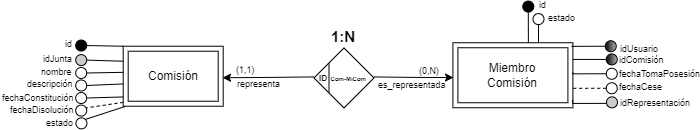
\includegraphics[scale=0.7]{img/diagramas/EER/I-Com-MiCom}
        \caption{Interrelación: Comisión - MiembroComisión}
        \label{fig:I-Com-MiCom}
    \end{figure}
    
    \item \textbf{Ejemplo} (Tabla \ref{table:I-Com-MiCom}).

    \begin{table}[H]
    \centering
        \begin{tabular}{ | c | c | c |  }
             \hline
                 \textbf{Entidad} & \textbf{Atributo} & \textbf{Ejemplo}\\       
             \hline
                 \textbf{Comisión}  & \underline{id} & 1\\
                  & id & 1\\
                  & idJunta & 1\\
                  & nombre & Asuntos económicos\\
                  & descripción & Economía de la comisión\\
                  & fechaConstitución & 10/09/2023\\
                  & fechaDisolución & null\\
                  & estado & 1\\
              \hline
                 \textbf{Miembro Comisión}  & \underline{id} & 1\\
                  & idUsuario & 1\\
                  & idComisión & 1\\
                  & idRepresentación & 2\\
                  & fechaTomaPosesión & 10/09/2023\\
                  & fechaCese & null\\
                  & estado & 1\\
        \end{tabular}
        \caption{Ejemplo de la interrelación \textit{Comisión - MiembroComisión}}
        \label{table:I-Com-MiCom}
    \end{table}
\end{itemize}

\subsection{Interrelación: Comisión - Convocatoria}
\begin{itemize}
    \item \textbf{Nombre}: Com-Conv.
    \item \textbf{Descripción}: esta interrelación muestra que una comisión puede gestionar cero, uno o más convocatorias, pero una convocatoria solamente puede ser gestionada por una comisión.
    \item \textbf{Tipo}: la entidad Convocatoria presenta una debilidad por identificación respecto de la entidad Comisión.
    \item \textbf{Cardinalidad}. 1:N
    \begin{itemize}
        \item Cardinalidad de Comisión (0,n): una comisión puede tener asociados 0, 1 o varias convocatorias.
        \item Cardinalidad de Convocatoria (1,1): una convocatoria solamente está asociado a una comisión.
    \end{itemize}
    \item \textbf{Atributos}: ninguno
    \item \textbf{Diagrama} (Figura \ref{fig:I-Com-Conv}) 
    \begin{figure}[H]
        \centering
        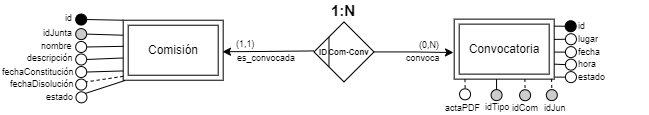
\includegraphics[scale=0.7]{img/diagramas/EER/I-Com-Conv}
        \caption{Interrelación: Comisión - Convocatoria}
        \label{fig:I-Com-Conv}
    \end{figure}
    
    \item \textbf{Ejemplo} (Tabla \ref{table:I-Com-Conv}).

    \begin{table}[H]
    \centering
        \begin{tabular}{ | c | c | c |  }
             \hline
                 \textbf{Entidad} & \textbf{Atributo} & \textbf{Ejemplo}\\       
             \hline
                 \textbf{Comisión}  & \underline{id} & 1\\
                  & id & 1\\
                  & idJunta & 1\\
                  & nombre & Asuntos económicos\\
                  & descripción & Economía de la comisión\\
                  & fechaConstitución & 10/09/2023\\
                  & fechaDisolución & null\\
                  & estado & 1\\
              \hline
                  \textbf{Convocatoria}  & \underline{id} & 1\\
                  & lugar & Rectorado\\
                  & fecha & 23/09/2023\\
                  & hora & 11:30\\
                  & idTipo & 1\\
                  & idComision & null\\
                  & idJunta & 1\\
                  & acta & /resources/actas/1.pdf \\
                  & estado & 1\\
        \end{tabular}
        \caption{Ejemplo de la interrelación \textit{Comisión - Convocatoria}}
        \label{table:I-Com-Conv}
    \end{table}
\end{itemize}

\subsection{Interrelación: Usuario - MiembroGobierno}
\begin{itemize}
    \item \textbf{Nombre}: Usu-MiGob.
    \item \textbf{Descripción}: esta interrelación muestra que un usuario puede corresponder a cero, uno o más miembros de gobierno, pero un miembro de gobierno solamente puede ser un usuario.
    \item \textbf{Tipo}: la entidad MiembroGobierno presenta una debilidad por identificación respecto de la entidad Usuario.
    \item \textbf{Cardinalidad}. 1:N
    \begin{itemize}
        \item Cardinalidad de Usuario (0,n): un usuario puede tener asociados 0, 1 o varias miembros de gobierno.
        \item Cardinalidad de MiembroGobierno (1,1): un miembro de gobierno solamente está asociado a un usuario.
    \end{itemize}
    \item \textbf{Atributos}: ninguno
    \item \textbf{Diagrama} (Figura \ref{fig:I-Usu-MiGob}) 
    \begin{figure}[H]
        \centering
        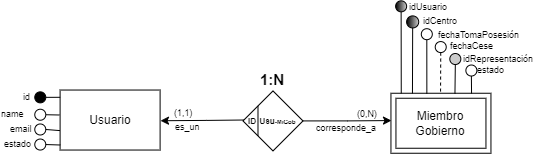
\includegraphics[scale=0.7]{img/diagramas/EER/I-Usu-MiGob}
        \caption{Interrelación: Usuario - MiembroGobierno}
        \label{fig:I-Usu-MiGob}
    \end{figure}
    
    \item \textbf{Ejemplo} (Tabla \ref{table:I-Usu-MiGob}).

    \begin{table}[H]
    \centering
        \begin{tabular}{ | c | c | c |  }
             \hline
                 \textbf{Entidad} & \textbf{Atributo} & \textbf{Ejemplo}\\       
             \hline
                 \textbf{Usuario}  & \underline{id} & 1\\
                  & id & 1\\
                  & name & Manuel Cañas Ramírez\\
                  & email & epsc.director@uco.es\\
                  & password & 2y$10$92IXUNpkjO0rOQ\\
                  & estado & 1\\
              \hline
                  \textbf{Miembro Gobierno}  & \underline{id} & 1\\
                  & idUsuario & 1\\
                  & idCentro & 1\\
                  & idRepresentación & 1\\
                  & fechaTomaPosesión & 10/09/2023\\
                  & fechaCese & null\\
                  & estado & 1\\
        \end{tabular}
        \caption{Ejemplo de la interrelación \textit{Usuario - MiembroGobierno}}
        \label{table:I-Usu-MiGob}
    \end{table}
\end{itemize}

\subsection{Interrelación: Usuario - MiembroJunta}
\begin{itemize}
    \item \textbf{Nombre}: Usu-MiJu.
    \item \textbf{Descripción}: esta interrelación muestra que un usuario puede corresponder a cero, uno o más miembros de junta, pero un miembro de junta solamente puede ser un usuario.
    \item \textbf{Tipo}: la entidad MiembroJunta presenta una debilidad por identificación respecto de la entidad Usuario.
    \item \textbf{Cardinalidad}. 1:N
    \begin{itemize}
        \item Cardinalidad de Usuario (0,n): un usuario puede tener asociados 0, 1 o varias miembros de junta.
        \item Cardinalidad de MiembroJunta (1,1): un miembro de junta solamente está asociado a un usuario.
    \end{itemize}
    \item \textbf{Atributos}: ninguno
    \item \textbf{Diagrama} (Figura \ref{fig:I-Usu-MiJu}) 
    \begin{figure}[H]
        \centering
        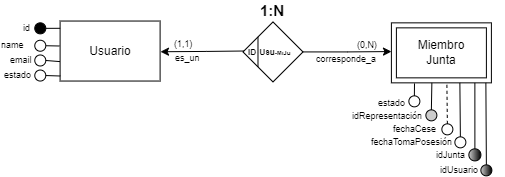
\includegraphics[scale=0.7]{img/diagramas/EER/I-Usu-MiJu}
        \caption{Interrelación: Usuario - MiembroJunta}
        \label{fig:I-Usu-MiJu}
    \end{figure}
    
    \item \textbf{Ejemplo} (Tabla \ref{table:I-Usu-MiJu}).

    \begin{table}[H]
    \centering
        \begin{tabular}{ | c | c | c |  }
             \hline
                 \textbf{Entidad} & \textbf{Atributo} & \textbf{Ejemplo}\\       
             \hline
                 \textbf{Usuario}  & \underline{id} & 1\\
                  & id & 1\\
                  & name & Manuel Cañas Ramírez\\
                  & email & epsc.director@uco.es\\
                  & password & 2y$10$92IXUNpkjO0rOQ\\
                  & estado & 1\\
              \hline
                  \textbf{Miembro Junta}  & \underline{id} & 1\\
                  & idUsuario & 1\\
                  & idJunta & 1\\
                  & idRepresentación & 1\\
                  & fechaTomaPosesión & 10/09/2023\\
                  & fechaCese & null\\
                  & estado & 1\\
        \end{tabular}
        \caption{Ejemplo de la interrelación \textit{Usuario - MiembroJunta}}
        \label{table:I-Usu-MiJu}
    \end{table}
\end{itemize}

\subsection{Interrelación: Usuario - MiembroComisión}
\begin{itemize}
    \item \textbf{Nombre}: Usu-MiCom.
    \item \textbf{Descripción}: esta interrelación muestra que un usuario puede corresponder a cero, uno o más miembros de comisión, pero un miembro de comisión solamente puede ser un usuario.
    \item \textbf{Tipo}: la entidad MiembroComisión presenta una debilidad por identificación respecto de la entidad Usuario.
    \item \textbf{Cardinalidad}. 1:N
    \begin{itemize}
        \item Cardinalidad de Usuario (0,n): un usuario puede tener asociados 0, 1 o varias miembros de comisión.
        \item Cardinalidad de MiembroComisión (1,1): un miembro de comisión solamente está asociado a un usuario.
    \end{itemize}
    \item \textbf{Atributos}: ninguno
    \item \textbf{Diagrama} (Figura \ref{fig:I-Usu-MiCom}) 
    \begin{figure}[H]
        \centering
        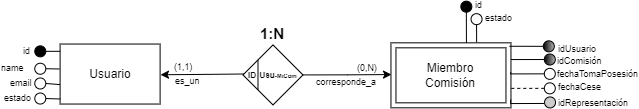
\includegraphics[scale=0.7]{img/diagramas/EER/I-Usu-MiCom}
        \caption{Interrelación: Usuario - MiembroComisión}
        \label{fig:I-Usu-MiCom}
    \end{figure}
    
    \item \textbf{Ejemplo} (Tabla \ref{table:I-Usu-MiCom}).

    \begin{table}[H]
    \centering
        \begin{tabular}{ | c | c | c |  }
             \hline
                 \textbf{Entidad} & \textbf{Atributo} & \textbf{Ejemplo}\\       
             \hline
                 \textbf{Usuario}  & \underline{id} & 1\\
                  & id & 1\\
                  & name & Manuel Cañas Ramírez\\
                  & email & epsc.director@uco.es\\
                  & password & 2y$10$92IXUNpkjO0rOQ\\
                  & estado & 1\\
              \hline
                  \textbf{Miembro Comisión}  & \underline{id} & 1\\
                  & idUsuario & 1\\
                  & idComisión & 1\\
                  & idRepresentación & 1\\
                  & fechaTomaPosesión & 10/09/2023\\
                  & fechaCese & null\\
                  & estado & 1\\
        \end{tabular}
        \caption{Ejemplo de la interrelación \textit{Usuario - MiembroComisión}}
        \label{table:I-Usu-MiCom}
    \end{table}
\end{itemize}

\begin{landscape}
\section{Diagrama del Modelo Entidad-Interrelación}\label{sec:diagrama-E-R}
El diagrama completo se muestra en la figura \ref{fig:EER_v5}
\begin{figure}[H]
    \centering
    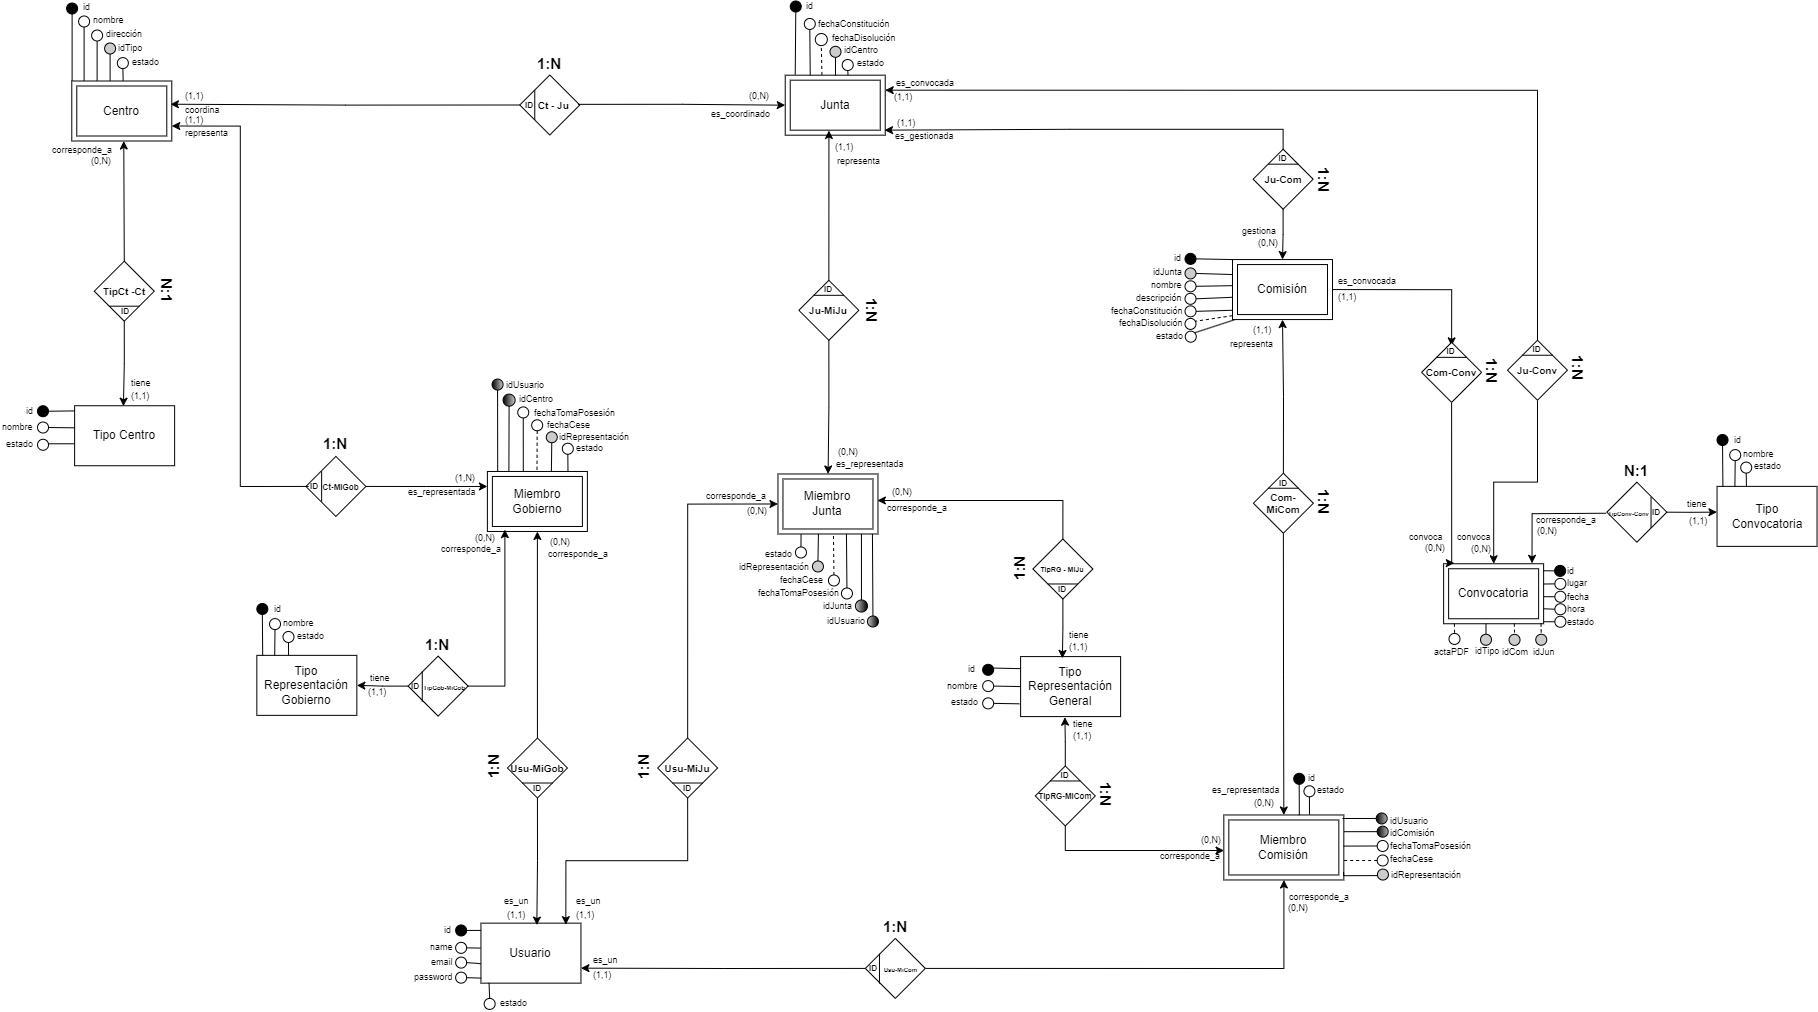
\includegraphics[scale=0.35]{img/diagramas/EER/EER_v5.png}
    \caption{Diagrama del modelo Entidad - Interrelación}
    \label{fig:EER_v5}
\end{figure}
\end{landscape}

\chapter{Análisis funcional} \label{cap:analisis}

\section{Introducción}

Este capítulo identificará a los tipos de actores que podrán interactuar con el sistema informático que se desea desarrollar. A continuación, se utilizarán los casos de uso y los diagramas de secuencia para describir las acciones que podrán realizar los diferentes actores.

\section{Actores}

Un actor es una representación de una persona, proceso o entidad externa que interactúa con el sistema. Se van a considerar seis tipos de actores:
    \begin{itemize}
        \item Administrador
          \begin{itemize}
              \item Este tipo de usuario estará registrado en el sistema y tendrá un control completo de la aplicación. 
              \item En particular, tendrá las competencias exclusivas de la gestión de todos los tipos de usuarios, centros, juntas, miembros y comisiones. Además, se encargará de la gestión de las copias de seguridad.
          \end{itemize}
          \item Responsable del centro
           \begin{itemize}
               \item Este tipo de usuario estará registrado en el sistema y representará a una persona que podrá gestionar la información de un centro.
               \item En particular, tendrá las competencias exclusivas de la asignación/exclusión a los miembros de gobierno pertenecientes a dicho centro, de creación de las juntas que pertenezcan al centro, así como asignación/exclusión del responsable de cada junta.
            \end{itemize}
            \item Responsable de la junta
           \begin{itemize}
               \item Este tipo de usuario estará registrado en el sistema y representará a una persona que podrá gestionar la información de una junta de centro.
               \item En particular, tendrá las competencias exclusivas de la asignación/exclusión a los miembros de junta pertenecientes a dicha junta, de la gestión de las convocatorias realizadas por la junta, de los miembros que participarán en cada una de las convocatorias de la junta, de creación de las comisiones que pertenezcan a la junta, así como asignación/exclusión del responsable de cada comisión.
            \end{itemize}
          \item Responsable de la comisión 
           \begin{itemize}
               \item Este tipo de usuario estará registrado en el sistema y representará a una persona que podrá gestionar la información de una comisión.
               \item En particular, tendrá las competencias exclusivas de la asignación/exclusión a los miembros pertenecientes a dicha comisión, gestión de las convocatorias realizadas por la comisión, y de los miembros que participarán en cada una de las convocatorias de dicha comisión.
            \end{itemize}
        \item Usuario universitario
            \begin{itemize}
                \item Este tipo de usuario estará registrado en el sistema.
                \item Podrá obtener distintos certificados como pueden ser de situación actual, de centros en los que ha participado como miembro de equipo de gobierno, de juntas a las que ha representado, de comisiones a las que ha pertenecido, de convocatorias en las que ha participado...
              \end{itemize}
        \item Público
        \begin{itemize}
              \item Este tipo de usuario no necesitará estar registrado en el sistema.
              \item Podrá consultar la información pública disponible: comisiones de un centro, miembros actuales de una comisión, consulta de actas aprobadas y pendientes de aprobación,...
          \end{itemize}
     \end{itemize}

\section{Casos de uso}

  Los casos de uso describen las acciones que pueden desarrollar los actores del sistema. Se ha identificado los siguientes casos de uso principales, que son descritos en las secciones que se indican:
    \begin{itemize}
    \item \textbf{CU-0. Diagrama de contexto} (Sección \ref{sec:CU-0}).  
    \item \textbf{CU-1. Consultar información pública} (Sección \ref{sec:CU-1}). 
    \item \textbf{CU-2. Administrar información de usuario} (Sección \ref{sec:CU-2}).
    \item \textbf{CU-3. Administrar comisión} (Sección \ref{sec:CU-3}).
    \item \textbf{CU-4. Administrar junta} (Sección \ref{sec:CU-4}).
    \item \textbf{CU-5. Administrar centro} (Sección \ref{sec:CU-5}).
    \item \textbf{CU-6. Administrar Sistema} (Sección \ref{sec:CU-6}).
\end{itemize}

\subsection{Caso de Uso 0. Diagrama de Contexto}\label{sec:CU-0}         

  El diagrama de contexto engloba los casos de uso principales que componen el sistemas. Véanse la Figura \ref{fig:Diagrama-Contexto} y la Tabla \ref{tab:CU-0}.

%Diagrama de contexto
\begin{figure}[H]
        \centering
        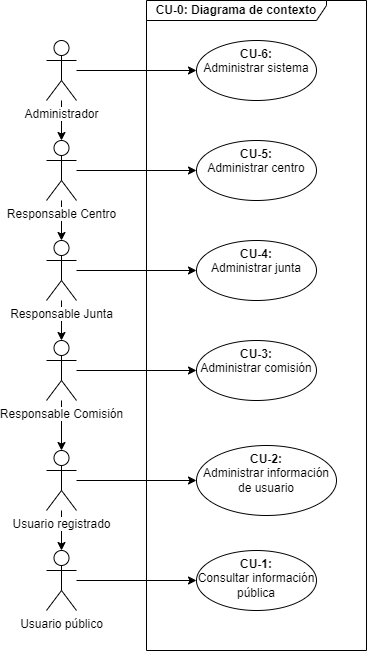
\includegraphics[scale=0.6]{img/diagramas/Funcional/CU-0.png}
        \caption{Diagrama de Contexto}\label{fig:Diagrama-Contexto}
\end{figure}

\begin{table}[H]
\caption{CU-0. Diagrama de contexto}\label{tab:CU-0}
\begin{center}
    \begin{tabular}{|l|p{12cm}|}
    \hline
    \multicolumn{2}{|c|}{Caso de uso 0 - Diagrama de contexto} \\ 
    \hline \hline
    Actores                 &   Público, Usuario registrado, Responsable Comisión,\\ 
                            &  Responsable Junta,  Responsable Centro, Administrador \\ \hline
    Descripción             &   Acciones principales del sistema\\  \hline
    Precondiciones          &   El usuario debe acceder a la página inicial de la aplicación   \\  \hline
    Casos de uso            &   CU-1. Consultar información pública\\  
    & CU-2. Administrar información de usuario\\ 
    & CU-3. Administrar comisión\\
    & CU-4. Administrar junta \\
    & CU-5. Administrar centro \\
    & CU-6. Administrar sistema \\
    \hline
    Flujo principal     &  1a. El usuario público accede a la aplicación sin necesidad de iniciar sesión y podrá consultar la información pública. \\
        & 1b. El resto de usuarios se deberá identificar para acceder a los módulos correspondientes dentro de la aplicación.
    \\ \hline
    Flujo alternativo    & 1. La aplicación no se carga correctamente. \\
      & 2. Se informa del error al usuario. \\
      & 3. Se informa al usuario que puede intentar cargar de nuevo la aplicación.
    \\  \hline
    \end{tabular}
    \end{center}
    \end{table}

\newpage

\subsection{CU-1. Consultar información pública}\label{sec:CU-1}

El caso de uso \textit{CU-1. Consultar información pública} describe las acciones que puede realizar el Usuario Público (véanse la Tabla \ref{tab:CU-1} y la Figura \ref{fig:Diagrama-Caso de uso 1. Consultar información pública}.). Este caso de uso está compuesto por los siguientes sub-casos de uso que se describen en las tablas que se indican:
\begin{itemize}
    \item CU-1.1 Consultar información actual equipos de gobierno(Tabla \ref{tab:CU-1.1}).
    \item CU-1.2 Consultar información actual junta (Tabla \ref{tab:CU-1.2}).
    \item CU-1.3 Consultar información actual comisiones (Tabla \ref{tab:CU-1.3}).
    \item CU-1.4 Consultar información actual convocatorias (Tabla \ref{tab:CU-1.4}).
    \item CU-1.5 Consultar ayuda usuario público (Tabla \ref{tab:CU-1.5}).
\end{itemize}

\begin{figure}[H]
\centering
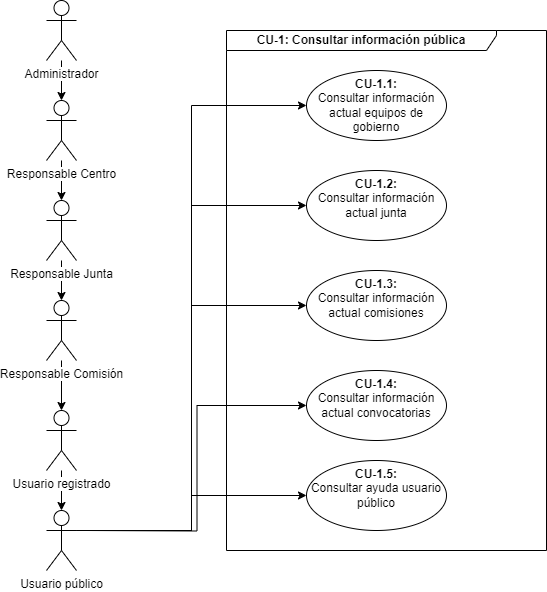
\includegraphics[scale=0.75]{img/diagramas/Funcional/CU-1.png}
\caption{CU-1. Consultar información pública}\label{fig:Diagrama-Caso de uso 1. Consultar información pública}   
\end{figure}

\begin{table}[H]
\caption{CU-1. Consultar información pública}\label{tab:CU-1}
\begin{center}
    \begin{tabular}{|l|p{12cm}|}
    \hline
    \multicolumn{2}{|c|}{Caso de uso 1 - Consultar información pública} \\ 
    \hline \hline
    Actores                 &   Usuario público          \\ \hline
    Descripción             &   Acciones que puede realizar el usuario público \\  \hline
    Precondiciones          &   El usuario debe haber accedido a la página principal de la aplicación y elegido el caso de uso CU-1. Consultar información pública.   \\  \hline
    Casos de uso            &   CU-1.1. Consultar información actual equipos de gobierno \\  
    & CU-1.2. Consultar información actual junta \\ 
    & CU-1.3. Consultar información actual comisiones \\
    & CU-1.4. Consultar información actual convocatorias \\
    & CU-1.5. Consultar ayuda usuario público\\

    \hline
    Flujo principal     &   1. El usuario elige un centro universitario \\ 
    & 2. El sistema muestra la información solicitada en formato organigrama \\ \hline
    Flujo alternativo    &  1. Se produce un error al intentar ejecutar la información elegida. \\ 
                            &  2. Se informa al usuario del error.  \\  
                            &  3. El sistema vuelve a mostrar las opciones disponibles.  \\  \hline    
            \end{tabular}
        \end{center}
    \end{table}

\begin{table}[H]
\caption{CU-1.1 Consultar información actual equipos de gobierno}
        \label{tab:CU-1.1}
        \begin{center}
            \begin{tabular}{|l|p{12cm}|}
                \hline
                \multicolumn{2}{|c|}{Caso de uso 1.1 - Consultar información actual equipos de gobierno} \\ \hline \hline
                Actores                 &   Usuario público          \\  \hline
                Descripción             &   Consultar información pública del equipo de gobierno actual de un centro seleccionado. \\  \hline
                Precondiciones          &   El usuario debe haber accedido a la aplicación y elegido el caso de uso CU-1.1 Consultar información actual equipos de gobierno.  \\  \hline
                Casos de uso            &   \\  \hline
                Flujo principal         &   1. El sistema muestra los centros universitarios   \\
                                        &   2. El usuario escoge un centro universitario    \\ 
                       & 3. El sistema muestra la información pública actual del centro escogido en formato organigrama \\ \hline
                Flujo alternativo    &   1. Se produce un error al intentar mostrar la información de un  centro no universitario. 
                \\  & 2. El sistema informa al usuario de error producido. 
                \\  & 3. El sistema vuelve a mostrar la lista de centros no universitarios.
                \\\hline
            \end{tabular}
        \end{center}
    \end{table}
    
\begin{table}[H]
\caption{CU-1.2 Consultar información actual junta}  \label{tab:CU-1.2}
        \begin{center}
            \begin{tabular}{|l|p{12cm}|}
                \hline
                \multicolumn{2}{|c|}{Caso de uso 1.2 - Consultar información actual junta} \\ \hline \hline
                Actores           &   Usuario público          \\  \hline
                Descripción         &   Consultar información actual junta. \\  \hline
                Precondiciones          &   El usuario debe haber accedido a la aplicación y elegido el caso de uso CU-1.2 Consultar información actual junta  \\  \hline
                Casos de uso            &          \\  \hline
                Flujo principal         &   1. El sistema muestra los centros universitarios.   \\
                &   2. El usuario escoge un centro universitario.    \\                  & 3. El sistema muestra la información pública actual del centro escogido. \\ \hline
                 Flujo alternativo    &   1. Se produce un error al intentar mostrar la información de un  centro  universitario. 
                \\  & 2. El sistema informa al usuario de error producido. 
                \\  & 3. El sistema vuelve a mostrar la lista de centros  universitarios. 
                \\
                \hline
            \end{tabular}
        \end{center}
    \end{table}

\begin{table}[H]
\caption{CU-1.3 Consultar información actual comisiones}  \label{tab:CU-1.3}
        \begin{center}
            \begin{tabular}{|l|p{12cm}|}
                \hline
                \multicolumn{2}{|c|}{Caso de uso 1.3 - Consultar información actual comisiones} \\ \hline \hline
                Actores           &   Usuario público          \\  \hline
                Descripción         &   Consultar información actual comisiones. \\  \hline
                Precondiciones          &   El usuario debe haber accedido a la aplicación y elegido el caso de uso CU-1.3 Consultar información actual comisiones  \\  \hline
                Casos de uso            &          \\  \hline
                Flujo principal         &   1. El sistema muestra los centros universitarios.   \\
                &   2. El usuario escoge un centro universitario.    \\                  & 3. El sistema muestra la información pública actual del centro escogido. \\ \hline
                 Flujo alternativo    &   1. Se produce un error al intentar mostrar la información de un  centro  universitario. 
                \\  & 2. El sistema informa al usuario de error producido. 
                \\  & 3. El sistema vuelve a mostrar la lista de centros  universitarios. 
                \\
                \hline
            \end{tabular}
        \end{center}
    \end{table}

\begin{table}[H]
\caption{CU-1.4 Consultar información actual convocatorias}  \label{tab:CU-1.4}
        \begin{center}
            \begin{tabular}{|l|p{12cm}|}
                \hline
                \multicolumn{2}{|c|}{Caso de uso 1.4 - Consultar información actual convocatorias} \\ \hline \hline
                Actores           &   Usuario público          \\  \hline
                Descripción         &   Consultar información actual convocatorias. \\  \hline
                Precondiciones          &   El usuario debe haber accedido a la aplicación y elegido el caso de uso CU-1.4 Consultar información actual convocatorias  \\  \hline
                Casos de uso            &          \\  \hline
                Flujo principal         &   1. El sistema muestra los centros universitarios.   \\
                &   2. El usuario escoge un centro universitario.    \\                  & 3. El sistema muestra la información pública actual del centro escogido. \\ \hline
                 Flujo alternativo    &   1. Se produce un error al intentar mostrar la información de un  centro  universitario. 
                \\  & 2. El sistema informa al usuario de error producido. 
                \\  & 3. El sistema vuelve a mostrar la lista de centros  universitarios. 
                \\
                \hline
            \end{tabular}
        \end{center}
    \end{table}

\begin{table}[H]
\caption{CU 1.5. Consultar ayuda del usuario público}        \label{tab:CU-1.5}
        \begin{center}
            \begin{tabular}{|l|p{12cm}|}
                \hline
                \multicolumn{2}{|c|}{Caso de uso 1.5 - Consultar ayuda del usuario público} \\ \hline \hline
                Actores                 &   Usuario público \\  \hline
                Descripción             &   Consultar ayuda del usuario público. \\  \hline
                Precondiciones          &  El usuario debe haber accedido a la aplicación y elegido el caso de uso CU-1.5 Consultar ayuda del usuario público. \\  \hline
                Casos de uso            &           \\  \hline
                Flujo principal         &   1. El sistema muestra la información de ayuda al usuario público \\ \hline
                Flujo alternativo    &   1. Se produce un error al intentar mostrar la ayuda al usuario. \\
                & 2. El sistema informa al usuario del error producido. \\
                & 3. El sistema vuelve a mostrar al usuario las opciones disponibles (CU-1. Consultar información pública).  \\
                \hline
            \end{tabular}
        \end{center}
    \end{table}

\newpage

\subsection{CU-2. Administrar información de usuario}\label{sec:CU-2}    

El caso de uso \textit{CU-2. Administrar información de usuario} describe las acciones que puede realizar el Usuario universitario registrado en el sistema (véanse la Tabla \ref{tab:CU-2} y la Figura \ref{fig:Diagrama-Caso de uso 2. Administrar información de usuario}.). Este caso de uso está compuesto por los siguientes sub-casos de uso que se describen en las tablas que se indican:
\begin{itemize}
    \item CU-2.1 Editar información de usuario (Tabla \ref{tab:CU-2.1}).
    \item CU-2.2 Generar certificados (Tabla \ref{tab:CU-2.2}).
    \item CU-2.3 Consultar ayuda (Tabla \ref{tab:CU-2.3}).
\end{itemize}

\begin{figure}[H]
        \centering
        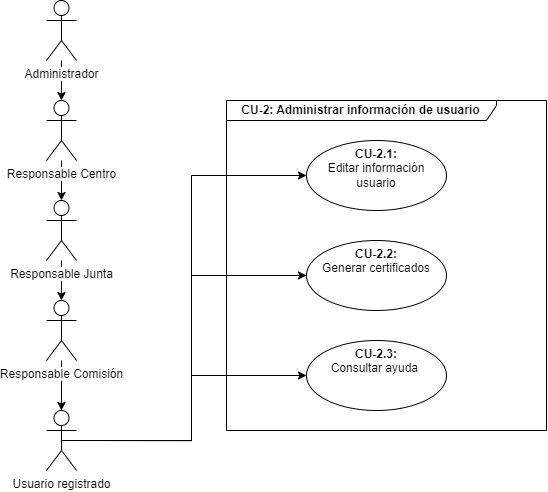
\includegraphics[scale=0.75]{img/diagramas/Funcional/CU-2.png}
        \caption{CU 2. Administrar información de usuario.}
        \label{fig:Diagrama-Caso de uso 2. Administrar información de usuario}
    \end{figure}

\begin{table}[H]
        \caption{CU-2. Administrar información de usuario}
        \label{tab:CU-2}
        \begin{center}
            \begin{tabular}{|l|p{12cm}|}
                \hline
                \multicolumn{2}{|c|}{Caso de uso 2 - Administrar información de usuario} \\ \hline \hline
                Actores                 &   Usuario universitario registrado        \\  \hline
                Descripción             &   Administrar información de usuario. \\  \hline
                Precondiciones          &   El usuario se debe haber identificado como usuario universitario y elegido el caso de uso CU-2 Administrar información de usuario.  \\  \hline
                Casos de uso            &  CU-2.1. Editar información usuario\\ 
                &
                CU-2.2. Generar certificados\\ 
                &
                CU-2.3. Consultar ayuda usuario universitario \\
                \hline
                Flujo principal     &    1. El sistema muestra al usuario universitario las opciones disponibles.\\ 
                &   2. El usuario elige una de las opciones.\\ 
                &   3. El sistema ejecuta la opción elegida por el usuario.\\ 
                \hline
                Flujo alternativo    &  1. Se produce un error al intentar ejecutar la opción elegida. \\ 
                &  2. Se informa al usuario del error.  \\  
                &  3. El sistema vuelve a mostrar las opciones disponibles.  \\
                \hline
            \end{tabular}
        \end{center}
    \end{table}


\begin{table}[H]
    \caption{CU-2.1. Editar información usuario}
    \label{tab:CU-2.1}
    \begin{center}
        \begin{tabular}{|l|p{12cm}|}
            \hline
            \multicolumn{2}{|c|}{Caso de uso 2.1 -Editar información usuario} \\ \hline \hline
            Actores                 &   Usuario universitario registrado          \\  \hline
            Descripción             &   Editar información  del usuario \\  \hline
            Precondiciones          &   El usuario se debe haber identificado como usuario universitario y elegido el caso de uso CU-2.1 Editar información usuario. \\
            \hline
            Casos de uso            &             \\  \hline
            Flujo principal         &   1. El sistema muestra en formato editable la información del usuario   \\
            &   2. El usuario edita la información que proceda.    \\ 
            & 3. El sistema graba los datos actualizados. \\ \hline
            Flujo alternativo    &   1. Se produce un error al editar la información. \\
            & 2. El sistema informa al usuario sobre el error que se ha producido. \\
            & 3. El sistema vuelve a mostrar la opción de editar la información del centro no universitario.
             \\  \hline
        \end{tabular}
    \end{center}
\end{table}

\begin{table}[H]
    \caption{CU-2.2. Generar certificados}
    \label{tab:CU-2.2}
    \begin{center}
        \begin{tabular}{|l|p{12cm}|}
            \hline
            \multicolumn{2}{|c|}{Caso de uso 2.2 -Generar certificados} \\ \hline \hline
            Actores                 &   Usuario universitario registrado          \\  \hline
            Descripción             &   Editar información  del usuario \\  \hline
            Precondiciones          &   El usuario se debe haber identificado como usuario universitario y elegido el caso de uso CU-2.2 Generar certificados. \\
            \hline
            Casos de uso            &             \\  \hline
            Flujo principal         &   1. El sistema muestra una lista de certificados a generar   \\
            &   2. El usuario selecciona el tipo de certificado.    \\ 
            & 3. El sistema genera un PDF con el tipo de certificado seleccionado por el usuario. \\ \hline
            Flujo alternativo    &   1. Se produce un error al seleccionar la información. \\
            & 2. El sistema informa al usuario sobre el error que se ha producido. \\
            & 3. El sistema vuelve a mostrar la opción de selección de la información.
             \\  \hline
        \end{tabular}
    \end{center}
\end{table}


\begin{table}[H]
\caption{CU 2.3. Consultar la ayuda del usuario universitario}        \label{tab:CU-2.3}
        \begin{center}
            \begin{tabular}{|l|p{12cm}|}
                \hline
                \multicolumn{2}{|c|}{Caso de uso 2.3 -  Consultar la ayuda del usuario universitario} \\
                \hline \hline
                Actores                 &   Usuario universitario registrado          \\  
                \hline
                Descripción             &   Consultar la ayuda del usuario universitario. \\  \hline
                Precondiciones          &  El usuario debe haber accedido a la aplicación y elegido el caso de uso CU-2.3 Consultar la ayuda del usuario universitario. \\  
                \hline
                Casos de uso            &           \\  
                \hline
                Flujo principal         &   1. El sistema muestra la información de ayuda al usuario  \\ 
                \hline
                Flujo alternativo    &   1. Se produce un error al intentar mostrar la ayuda del usuario. \\
                & 2. El sistema informa al usuario del error ocurrido. \\
                & 3. El sistema vuelve a mostrar al usuario las opciones disponibles (CU-2. Administrar centro no universitario).  \\
                \hline
            \end{tabular}
        \end{center}
    \end{table}
\newpage


\subsection{CU-3. Administrar comisión}\label{sec:CU-3}    
El caso de uso \textit{CU-3. Administrar comisión} describe las acciones que puede realizar el Usuario responsable de comisión (véanse la Tabla \ref{tab:CU-3} y la Figura \ref{fig:Diagrama-Caso de uso 3. Administrar comisión}). Este caso de uso está compuesto por los siguientes sub-casos de uso que se describen en las tablas que se indican:
\begin{itemize}
  \item CU-3.1 Editar información de comisión responsable (Tabla \ref{tab:CU-3.1}).
  \item CU-3.2 Gestionar miembros de comisión (Tabla \ref{tab:CU-3.2}).
          \begin{itemize}
            \item CU-3.2.1 Buscar miembro de comisión.
            \item CU-3.2.2 Crear  miembro de comisión.
            \item CU-3.2.3 Consultar miembro de comisión.
            \item CU-3.2.4 Modificar miembro de comisión.
            \item CU-3.2.5 Eliminar miembro de comisión.
            \item CU-3.2.6 Asignar/Desasignar responsable miembro de comisión.
        \end{itemize}
  \item CU-3.3 Gestionar convocatorias de comisión (Tabla \ref{tab:CU-3.3}).
          \begin{itemize}
            \item CU-3.3.1 Buscar convocatoria de comisión.
            \item CU-3.3.2 Crear convocatoria de comisión.
            \item CU-3.3.3 Consultar convocatoria de comisión.
            \item CU-3.3.4 Modificar convocatoria de comisión.
            \item CU-3.3.5 Eliminar convocatoria de comisión.
            \item CU-3.3.6 Asignar/Desasignar asistentes convocatoria de comisión.

        \end{itemize}
 \item CU-3.4 Consultar la ayuda del responsable comisión (Tabla \ref{tab:CU-3.4}).
\end{itemize}


\begin{figure}[H]
        \centering
        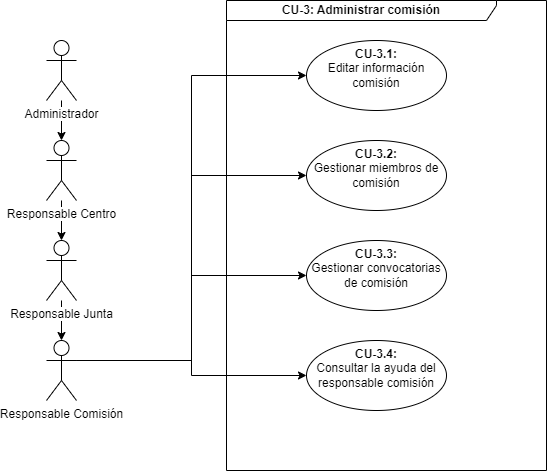
\includegraphics[scale=0.75]{img/diagramas/Funcional/CU-3.png}
        \caption{CU-3. Administrar comisión}
        \label{fig:Diagrama-Caso de uso 3. Administrar comisión}
    \end{figure}
    
\begin{table}[H]
        \caption{CU-3. Administrar comisión}
        \label{tab:CU-3}
        \begin{center}
            \begin{tabular}{|l|p{12cm}|}
                \hline
                \multicolumn{2}{|c|}{Caso de uso 3 - Administrar comisión} \\ \hline \hline
                Actores                 &   Responsable  comisión         \\  \hline
                Descripción             &   Gestión de una comisión. \\  \hline
                Precondiciones          &   El usuario se debe haber identificado como responsable comisión y elegido el caso de uso CU-3. Administrar comisión.  \\  \hline
                Casos de uso            &  CU-3.1. Editar información de comisión responsable. \\ 
                &
                CU-3.2. Gestionar miembros de comisión. \\ 
                &
                CU-3.3. Gestionar convocatorias de comisión. \\ 
                & 
                CU-3.4. Consultar la ayuda del responsable comisión. \\ 
                \hline
                Flujo principal     &    1. El sistema muestra al responsable comisión las opciones disponibles.\\ 
                &   2. El responsable comisión elige una de las opciones.\\ 
                &   3. El sistema ejecuta la opción elegida por el responsable comisión.\\ 
                \hline
                Flujo alternativo    &  1. Se produce un error al intentar ejecutar la opción elegida. \\ 
                &  2. Se informa al usuario del error.  \\  
                &  3. El sistema vuelve a mostrar las opciones disponibles.  \\
                \hline
            \end{tabular}
        \end{center}
    \end{table}

\begin{table}[H]
    \caption{CU-3.1. Editar información de comisión responsable}
    \label{tab:CU-3.1}
    \begin{center}
        \begin{tabular}{|l|p{12cm}|}
            \hline
            \multicolumn{2}{|c|}{Caso de uso 3.1 - Editar información de comisión responsable} \\ \hline \hline
            Actores                 &   Usuario responsable comisión          \\  \hline
            Descripción             &   Editar información  de la comisión. \\  \hline
            Precondiciones          &   El usuario se debe haber identificado como responsable comisión y elegido el caso de uso CU-3.1 Editar información de comisión responsable. \\
            \hline
            Casos de uso            &             \\  \hline
            Flujo principal         &   1. El sistema muestra en formato editable la información de la comisión   \\
            &   2. El responsable comisión edita la información que proceda.    \\ 
            & 3. El sistema graba los datos actualizados. \\ 
            \hline
            Flujo alternativo    &   1. Se produce un error al editar la información. \\
            & 2. El sistema informa al usuario sobre el error que se ha producido. \\
            & 3. El sistema vuelve a mostrar la opción de editar la información de la comisión. \\ 
            \hline
        \end{tabular}
    \end{center}
\end{table}


\begin{table}[H]
    \caption{Gestionar miembros de comisión}
    \label{tab:CU-3.2}
    \begin{center}
        \begin{tabular}{|l|p{12cm}|}
            \hline
            \multicolumn{2}{|c|}{Caso de uso 3.2 - Gestionar miembros de comisión} \\
            \hline \hline
            Actores                 &   Responsable de comisión          \\  
            \hline
            Descripción             &   Permite la gestión de los miembros de la comisión responsable. \\  \hline
            Precondiciones          &   El usuario se debe haber identificado como responsable comisión y elegido el caso de uso CU-3.2 Gestionar miembros de comisión. \\  \hline
            Casos de uso            & 
            3.2.1 Buscar miembro de comisión \\ 
            &
            3.2.2 Crear miembro de comisión \\ 
            & 
            3.2.3. Consultar miembro de comisión\\ 
            & 
            3.2.4 Modificar miembro de comisión \\ 
            &  
            3.2.5 Eliminar miembro de comisión \\ 
            &
            3.2.6 Asignar/Desasignar responsable miembro de comisión \\
            \hline
   
            Flujo principal         &   1. El sistema muestra la lista de los miembros de la comisión responsable.   \\ 
            & 2a. Si no encuentra el miembro de comisión que busca entonces puede crearlo. \\ 
            & 2b. Si encuentra el miembro de comisión que busca entonces puede consultarlo, modificarlo o borrarlo. \\ \hline
            Flujo alternativo    &   1. Se produce un error al intentar ejecutar la opción elegida.  \\ 
            & 2. Se informa del error al usuario. \\
            & 3. El sistema vuelve a mostrar las opciones disponibles. \\
            \hline
        \end{tabular}
    \end{center}
\end{table}

\begin{figure}[H]
        \centering
        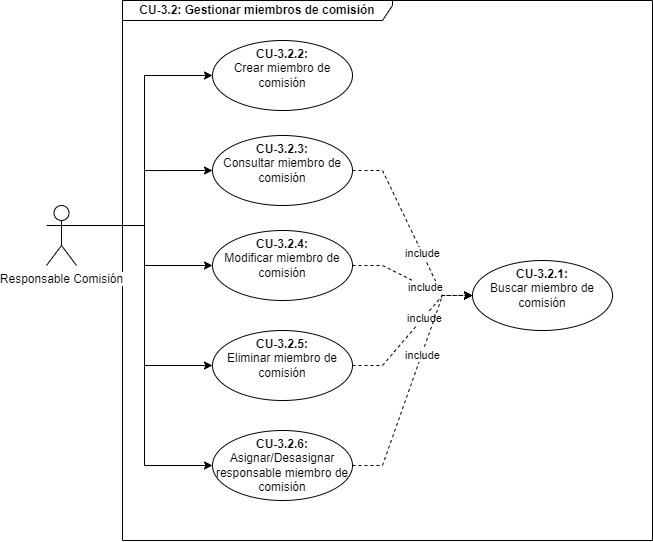
\includegraphics[scale=0.55]{img/diagramas/Funcional/CU-3.2.png}
        \caption{CU-3.2 Gestionar miembros de comisión}
        \label{fig:Diagrama-Caso de uso 3.2 Gestionar miembros de comisión}
    \end{figure}

\begin{table}[H]
    \caption{Gestionar convocatorias de comisión}
    \label{tab:CU-3.3}
    \begin{center}
        \begin{tabular}{|l|p{12cm}|}
            \hline
            \multicolumn{2}{|c|}{Caso de uso 3.3 - Gestionar convocatorias de comisión} \\
            \hline \hline
            Actores                 &   Responsable de comisión          \\  
            \hline
            Descripción             &   Permite la gestión de las convocatorias de la comisión responsable. \\  \hline
            Precondiciones          &   El usuario se debe haber identificado como responsable comisión y elegido el caso de uso CU-3.3 Gestionar convocatorias de comisión. \\  \hline
            Casos de uso            & 
            3.3.1 Buscar convocatoria \\ 
            &
            3.3.2 Crear convocatoria \\ 
            & 
            3.3.3. Consultar convocatoria\\ 
            & 
            3.3.4 Modificar convocatoria \\ 
            &  
            3.3.5 Eliminar convocatoria \\ 
            &
            3.3.6 Asignar/Desasignar asistentes convocatoria de comisión \\
            \hline
   
            Flujo principal         &   1. El sistema muestra la lista de las convocatorias de la comisión responsable.   \\ 
            & 2a. Si no encuentra la convocatoria de comisión que busca entonces puede crearla. \\ 
            & 2b. Si encuentra la convocatoria de comisión que busca entonces puede consultarla, modificarla o borrarla. \\ \hline
            Flujo alternativo    &   1. Se produce un error al intentar ejecutar la opción elegida.  \\ 
            & 2. Se informa del error al usuario. \\
            & 3. El sistema vuelve a mostrar las opciones disponibles. \\
            \hline
        \end{tabular}
    \end{center}
\end{table}

\begin{figure}[H]
        \centering
        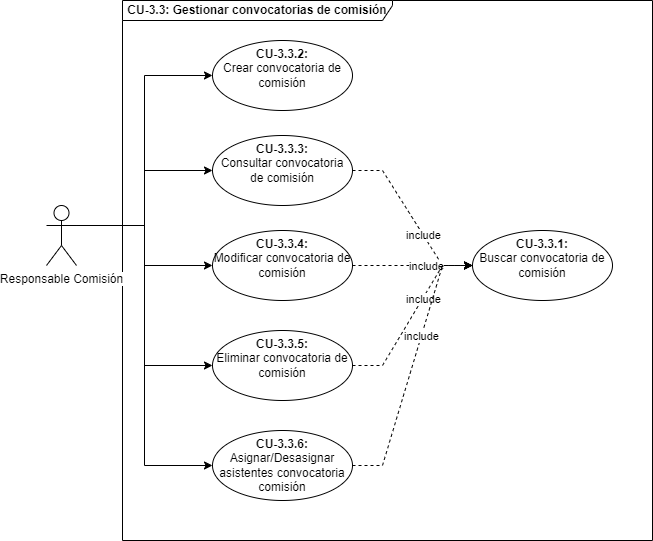
\includegraphics[scale=0.55]{img/diagramas/Funcional/CU-3.3.png}
        \caption{CU-3.3 Gestionar convocatorias de comisión}
        \label{fig:Diagrama-Caso de uso 3.3 Gestionar convocatorias de comisión}
    \end{figure}


\begin{table}[H]
    \caption{Consultar ayuda de responsable comisión}
    \label{tab:CU-3.4}
    \begin{center}
        \begin{tabular}{|l|p{12cm}|}
            \hline
            \multicolumn{2}{|c|}{Caso de uso 3.4 - Consultar ayuda de responsable comisión} \\ \hline 
            Actores                 &   Responsable comisión          \\  
            \hline
            Descripción        & Consultar ayuda de responsable comisión    \\ \hline 
            Precondiciones          &   El usuario debe identificarse  como responsable comisión y seleccionar el caso de uso CU-3.4 Consultar ayuda de responsable comisión         \\  \hline
            Casos de uso            &          \\ \hline
            Flujo principal         &   1. El sistema muestra la información de ayuda 
            al usuario responsable comisión.     \\\hline
            Flujo alternativo    &   1. Se produce un error al intentar mostrar la ayuda del usuario \\ 
            & 2. El sistema informa al usuario del error ocurrido. \\ 
            & 3. El sistema vuelve a mostrar al usuario las opciones disponibles (CU-3. Administrar comisión).\\  \hline
        \end{tabular}
    \end{center}
\end{table}

\newpage


\subsection{CU-4. Administrar junta}\label{sec:CU-4}    
El caso de uso \textit{CU-4. Administrar junta} describe las acciones que puede realizar el Usuario responsable de junta (véanse la Tabla \ref{tab:CU-4} y la Figura \ref{fig:Diagrama-Caso de uso 4. Administrar junta}). Este caso de uso está compuesto por los siguientes sub-casos de uso que se describen en las tablas que se indican:
\begin{itemize}
  \item CU-4.1 Editar información de comisión responsable (Tabla \ref{tab:CU-4.1}).
   \item CU-4.2 Gestionar comisiones (Tabla \ref{tab:CU-4.2}).
          \begin{itemize}
            \item CU-4.2.1 Buscar comisión.
            \item CU-4.2.2 Crear comisión.
            \item CU-4.2.3 Consultar comisión.
            \item CU-4.2.4 Modificar comisión.
            \item CU-4.2.5 Eliminar comisión.
        \end{itemize}
  \item CU-4.3 Gestionar miembros de junta (Tabla \ref{tab:CU-4.3}).
          \begin{itemize}
            \item CU-4.3.1 Buscar miembro de junta.
            \item CU-4.3.2 Crear  miembro de junta.
            \item CU-4.3.3 Consultar miembro de junta.
            \item CU-4.3.4 Modificar miembro de junta.
            \item CU-4.3.5 Eliminar miembro de junta.
            \item CU-4.3.6 Asignar/Desasignar responsable miembro de junta.
        \end{itemize}
    \item CU-4.4 Gestionar convocatorias de junta (Tabla \ref{tab:CU-4.4}).
          \begin{itemize}
            \item CU-4.4.1 Buscar convocatoria de junta.
            \item CU-4.4.2 Crear convocatoria de junta.
            \item CU-4.4.3 Consultar convocatoria de junta.
            \item CU-4.4.4 Modificar convocatoria de junta.
            \item CU-4.4.5 Eliminar convocatoria de junta.
            \item CU-4.4.6 Asignar/Desasignar asistentes convocatoria de junta.
        \end{itemize}
 \item CU-4.5 Consultar la ayuda del responsable junta (Tabla \ref{tab:CU-4.5}).
\end{itemize}


\begin{figure}[H]
        \centering
        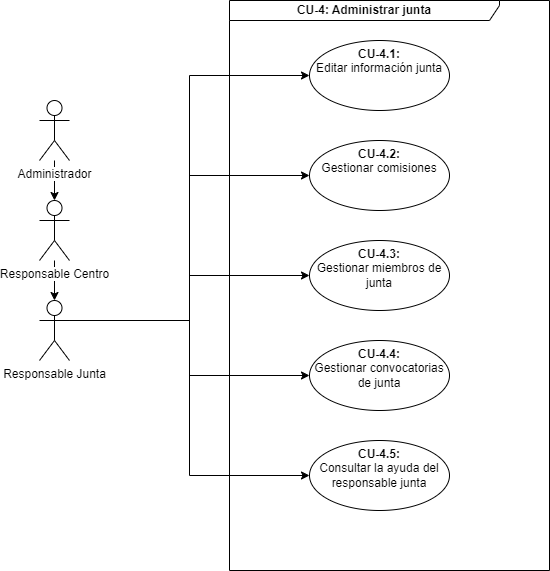
\includegraphics[scale=0.55]{img/diagramas/Funcional/CU-4.png}
        \caption{CU-4. Administrar junta}
        \label{fig:Diagrama-Caso de uso 4. Administrar junta}
    \end{figure}
    
\begin{table}[H]
        \caption{CU-4. Administrar junta}
        \label{tab:CU-4}
        \begin{center}
            \begin{tabular}{|l|p{12cm}|}
                \hline
                \multicolumn{2}{|c|}{Caso de uso 4 - Administrar junta} \\ \hline \hline
                Actores                 &   Responsable junta         \\  \hline
                Descripción             &   Gestión de una junta. \\  \hline
                Precondiciones          &   El usuario se debe haber identificado como responsable junta y elegido el caso de uso CU-4. Administrar junta.  \\  \hline
                Casos de uso            &  CU-4.1. Editar información de junta responsable. \\ 
                &
                CU-4.2. Gestionar comisiones. \\ 
                &
                CU-4.3. Gestionar miembros de junta. \\ 
                &
                CU-4.4. Gestionar convocatorias de junta. \\ 
                & 
                CU-4.5. Consultar la ayuda del responsable junta. \\ 
                \hline
                Flujo principal     &    1. El sistema muestra al responsable junta las opciones disponibles.\\ 
                &   2. El responsable junta elige una de las opciones.\\ 
                &   3. El sistema ejecuta la opción elegida por el responsable junta.\\ 
                \hline
                Flujo alternativo    &  1. Se produce un error al intentar ejecutar la opción elegida. \\ 
                &  2. Se informa al usuario del error.  \\  
                &  3. El sistema vuelve a mostrar las opciones disponibles.  \\
                \hline
            \end{tabular}
        \end{center}
    \end{table}

\begin{table}[H]
    \caption{CU-4.1. Editar información de junta}
    \label{tab:CU-4.1}
    \begin{center}
        \begin{tabular}{|l|p{12cm}|}
            \hline
            \multicolumn{2}{|c|}{Caso de uso 4.1 - Editar información de junta} \\ \hline \hline
            Actores                 &   Usuario responsable junta          \\  \hline
            Descripción             &   Editar información  de la junta. \\  \hline
            Precondiciones          &   El usuario se debe haber identificado como responsable junta y elegido el caso de uso CU-4.1 Editar información de junta responsable. \\
            \hline
            Casos de uso            &             \\  \hline
            Flujo principal         &   1. El sistema muestra en formato editable la información de la junta   \\
            &   2. El responsable junta edita la información que proceda.    \\ 
            & 3. El sistema graba los datos actualizados. \\ 
            \hline
            Flujo alternativo    &   1. Se produce un error al editar la información. \\
            & 2. El sistema informa al usuario sobre el error que se ha producido. \\
            & 3. El sistema vuelve a mostrar la opción de editar la información de la junta. \\ 
            \hline
        \end{tabular}
    \end{center}
\end{table}

\begin{table}[H]
    \caption{Gestionar comisiones}
    \label{tab:CU-4.2}
    \begin{center}
        \begin{tabular}{|l|p{12cm}|}
            \hline
            \multicolumn{2}{|c|}{Caso de uso 4.2 - Gestionar comisiones} \\
            \hline \hline
            Actores                 &   Responsable de junta          \\  
            \hline
            Descripción             &   Permite la gestión de las comisiones de la junta responsable. \\  \hline
            Precondiciones          &   El usuario se debe haber identificado como responsable junta y elegido el caso de uso CU-4.2 Gestionar comisiones de junta. \\  \hline
            Casos de uso            & 
            4.2.1 Buscar comisión \\ 
            &
            4.2.2 Crear comisión \\ 
            & 
            4.2.3. Consultar comisión\\ 
            & 
            4.2.4 Modificar comisión \\ 
            &  
            4.2.5 Eliminar comisión \\ 
            &
            4.2.6 Asignar/Desasignar responsable de comisión \\
            \hline
   
            Flujo principal         &   1. El sistema muestra la lista de las comisiones de la junta responsable.   \\ 
            & 2a. Si no encuentra la comisión que busca entonces puede crearla. \\ 
            & 2b. Si encuentra la comisión que busca entonces puede consultarla, modificarla o borrarla. \\ \hline
            Flujo alternativo    &   1. Se produce un error al intentar ejecutar la opción elegida.  \\ 
            & 2. Se informa del error al usuario. \\
            & 3. El sistema vuelve a mostrar las opciones disponibles. \\
            \hline
        \end{tabular}
    \end{center}
\end{table}

\begin{figure}[H]
        \centering
        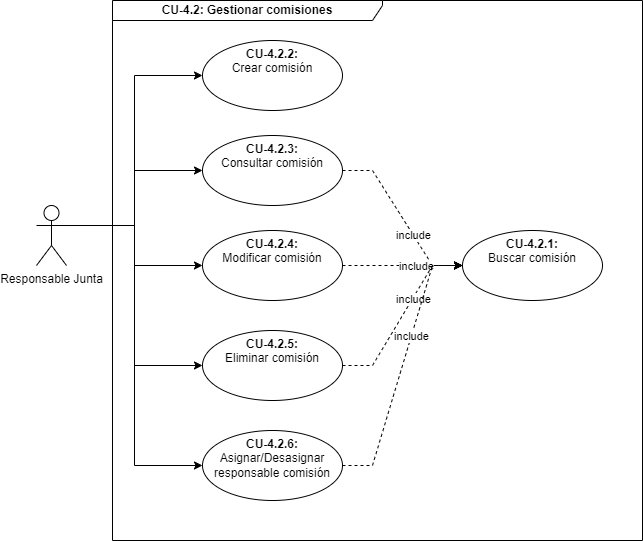
\includegraphics[scale=0.55]{img/diagramas/Funcional/CU-4.2.png}
        \caption{CU-4.2 Gestionar comisiones}
        \label{fig:Diagrama-Caso de uso 4.2 Gestionar comisiones}
    \end{figure}


\begin{table}[H]
    \caption{Gestionar miembros de junta}
    \label{tab:CU-4.3}
    \begin{center}
        \begin{tabular}{|l|p{12cm}|}
            \hline
            \multicolumn{2}{|c|}{Caso de uso 4.3 - Gestionar miembros de junta} \\
            \hline \hline
            Actores                 &   Responsable de junta          \\  
            \hline
            Descripción             &   Permite la gestión de los miembros de la junta responsable. \\  \hline
            Precondiciones          &   El usuario se debe haber identificado como responsable junta y elegido el caso de uso CU-4.3 Gestionar miembros de junta. \\  \hline
            Casos de uso            & 
            4.3.1 Buscar miembro de junta \\ 
            &
            4.3.2 Crear  miembro de junta \\ 
            & 
            4.3.3. Consultar miembro de junta\\ 
            & 
            4.3.4 Modificar miembro de junta \\ 
            &  
            4.3.5 Eliminar miembro de junta \\ 
            &
            4.3.6 Asignar/Desasignar responsable miembro de junta \\
            \hline
   
            Flujo principal         &   1. El sistema muestra la lista de los miembros de la junta responsable.   \\ 
            & 2a. Si no encuentra el miembro de junta que busca entonces puede crearlo. \\ 
            & 2b. Si encuentra el miembro de junta que busca entonces puede consultarlo, modificarlo o borrarlo. \\ \hline
            Flujo alternativo    &   1. Se produce un error al intentar ejecutar la opción elegida.  \\ 
            & 2. Se informa del error al usuario. \\
            & 3. El sistema vuelve a mostrar las opciones disponibles. \\
            \hline
        \end{tabular}
    \end{center}
\end{table}

\begin{figure}[H]
        \centering
        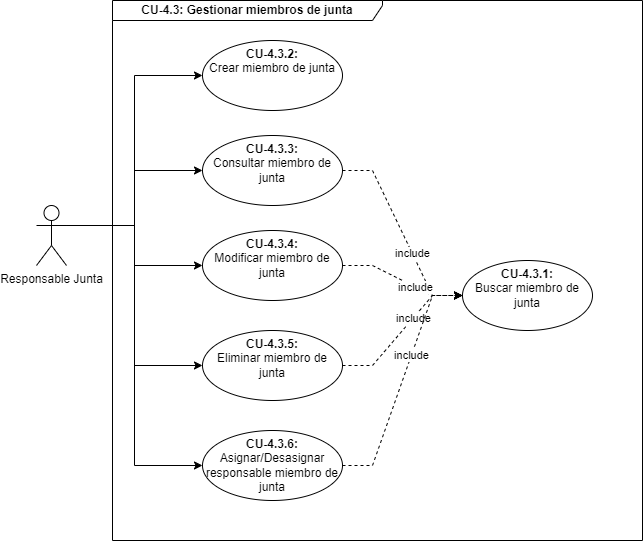
\includegraphics[scale=0.55]{img/diagramas/Funcional/CU-4.3.png}
        \caption{CU-4.3 Gestionar miembros de junta}
        \label{fig:Diagrama-Caso de uso 4.3 Gestionar miembros de junta}
    \end{figure}

\begin{table}[H]
    \caption{Gestionar convocatorias de junta}
    \label{tab:CU-4.4}
    \begin{center}
        \begin{tabular}{|l|p{12cm}|}
            \hline
            \multicolumn{2}{|c|}{Caso de uso 4.4 - Gestionar convocatorias de junta} \\
            \hline \hline
            Actores                 &   Responsable de junta          \\  
            \hline
            Descripción             &   Permite la gestión de las convocatorias de la junta responsable. \\  \hline
            Precondiciones          &   El usuario se debe haber identificado como responsable \textbf{comisión} y elegido el caso de uso CU-4.4 Gestionar convocatorias de junta. \\  \hline
            Casos de uso            & 
            4.4.1 Buscar convocatoria \\ 
            &
            4.4.2 Crear convocatoria \\ 
            & 
            4.4.3. Consultar convocatoria\\ 
            & 
            4.4.4 Modificar convocatoria \\ 
            &  
            4.4.5 Eliminar convocatoria \\ 
            &
            4.4.6 Asignar/Desasignar responsable convocatoria de junta \\
            \hline
   
            Flujo principal         &   1. El sistema muestra la lista de las convocatorias de la junta responsable.   \\ 
            & 2a. Si no encuentra la convocatoria de junta que busca entonces puede crearla. \\ 
            & 2b. Si encuentra la convocatoria de junta que busca entonces puede consultarla, modificarla o borrarla. \\ \hline
            Flujo alternativo    &   1. Se produce un error al intentar ejecutar la opción elegida.  \\ 
            & 2. Se informa del error al usuario. \\
            & 3. El sistema vuelve a mostrar las opciones disponibles. \\
            \hline
        \end{tabular}
    \end{center}
\end{table}

\begin{figure}[H]
        \centering
        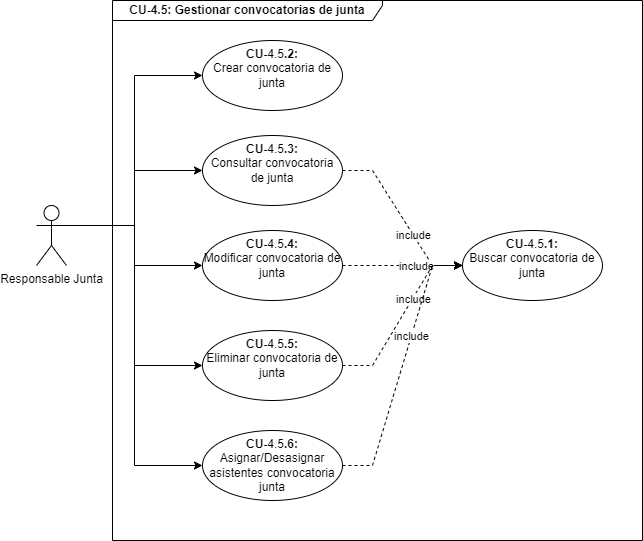
\includegraphics[scale=0.55]{img/diagramas/Funcional/CU-4.4.png}
        \caption{CU-4.4 Gestionar convocatorias de junta}
        \label{fig:Diagrama-Caso de uso 4.4 Gestionar convocatorias de junta}
    \end{figure}


\begin{table}[H]
    \caption{Consultar ayuda de responsable junta}
    \label{tab:CU-4.5}
    \begin{center}
        \begin{tabular}{|l|p{12cm}|}
            \hline
            \multicolumn{2}{|c|}{Caso de uso 4.5 - Consultar ayuda de responsable junta} \\ \hline 
            Actores                 &   Responsable junta          \\  
            \hline
            Descripción        & Consultar ayuda de responsable junta    \\ \hline 
            Precondiciones          &   El usuario debe identificarse  como responsable junta y seleccionar el caso de uso CU-4.5 Consultar ayuda de responsable junta         \\  \hline
            Casos de uso            &          \\ \hline
            Flujo principal         &   1. El sistema muestra la información de ayuda 
            al usuario responsable junta.     \\\hline
            Flujo alternativo    &   1. Se produce un error al intentar mostrar la ayuda del usuario \\ 
            & 2. El sistema informa al usuario del error ocurrido. \\ 
            & 3. El sistema vuelve a mostrar al usuario las opciones disponibles (CU-4. Administrar junta).\\  \hline
        \end{tabular}
    \end{center}
\end{table}

\newpage


\subsection{CU-5. Administrar centro}\label{sec:CU-5}    
El caso de uso \textit{CU-5. Administrar centro} describe las acciones que puede realizar el Usuario responsable de centro (véanse la Tabla \ref{tab:CU-5} y la Figura \ref{fig:Diagrama-Caso de uso 5. Administrar centro}). Este caso de uso está compuesto por los siguientes sub-casos de uso que se describen en las tablas que se indican:
\begin{itemize}
  \item CU-5.1 Editar información de centro responsable (Tabla \ref{tab:CU-5.1}).
  \item CU-5.2 Gestionar juntas (Tabla \ref{tab:CU-5.2}).
          \begin{itemize}
            \item CU-5.2.1 Buscar junta.
            \item CU-5.2.2 Crear junta.
            \item CU-5.2.3 Consultar junta.
            \item CU-5.2.4 Modificar junta.
            \item CU-5.2.5 Eliminar junta.
            \item CU-5.2.6 Asignar/Desasignar responsable de junta 

        \end{itemize}
  \item CU-5.3 Gestionar miembros de gobierno (Tabla \ref{tab:CU-5.3}).
          \begin{itemize}
            \item CU-5.3.1 Buscar miembro de gobierno.
            \item CU-5.3.2 Crear  miembro de gobierno.
            \item CU-5.3.3 Consultar miembro de gobierno.
            \item CU-5.3.4 Modificar miembro de gobierno.
            \item CU-5.3.5 Eliminar miembro de gobierno.
            \item CU-5.3.6 Asignar/Desasignar responsable miembro de gobierno.
        \end{itemize}
  
 \item CU-5.4 Consultar la ayuda del responsable centro (Tabla \ref{tab:CU-5.4}).
\end{itemize}


\begin{figure}[H]
        \centering
        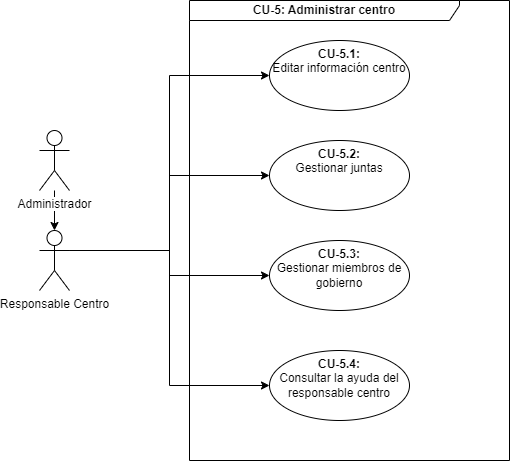
\includegraphics[scale=0.55]{img/diagramas/Funcional/CU-5.png}
        \caption{CU-5. Administrar centro}
        \label{fig:Diagrama-Caso de uso 5. Administrar centro}
    \end{figure}
    
\begin{table}[H]
        \caption{CU-5. Administrar centro}
        \label{tab:CU-5}
        \begin{center}
            \begin{tabular}{|l|p{12cm}|}
                \hline
                \multicolumn{2}{|c|}{Caso de uso 5 - Administrar centro} \\ \hline \hline
                Actores                 &   Responsable centro         \\  \hline
                Descripción             &   Gestión de un centro. \\  \hline
                Precondiciones          &   El usuario se debe haber identificado como responsable centro y elegido el caso de uso CU-5. Administrar centro.  \\  \hline
                Casos de uso            &  CU-5.1. Editar información de centro responsable. \\ 
                &
                CU-5.2. Gestionar juntas. \\ 
                &
                CU-5.3. Gestionar miembros de gobierno. \\ 
                &
                CU-5.4. Consultar la ayuda del responsable centro. \\ 
                \hline
                Flujo principal     &    1. El sistema muestra al responsable centro las opciones disponibles.\\ 
                &   2. El responsable centro elige una de las opciones.\\ 
                &   3. El sistema ejecuta la opción elegida por el responsable centro.\\ 
                \hline
                Flujo alternativo    &  1. Se produce un error al intentar ejecutar la opción elegida. \\ 
                &  2. Se informa al usuario del error.  \\  
                &  3. El sistema vuelve a mostrar las opciones disponibles.  \\
                \hline
            \end{tabular}
        \end{center}
    \end{table}

\begin{table}[H]
    \caption{CU-5.1. Editar información de centro}
    \label{tab:CU-5.1}
    \begin{center}
        \begin{tabular}{|l|p{12cm}|}
            \hline
            \multicolumn{2}{|c|}{Caso de uso 5.1 - Editar información de centro} \\ \hline \hline
            Actores                 &   Usuario responsable centro          \\  \hline
            Descripción             &   Editar información  de la centro. \\  \hline
            Precondiciones          &   El usuario se debe haber identificado como responsable centro y elegido el caso de uso CU-5.1 Editar información de centro responsable. \\
            \hline
            Casos de uso            &             \\  \hline
            Flujo principal         &   1. El sistema muestra en formato editable la información del centro   \\
            &   2. El responsable centro edita la información que proceda.    \\ 
            & 3. El sistema graba los datos actualizados. \\ 
            \hline
            Flujo alternativo    &   1. Se produce un error al editar la información. \\
            & 2. El sistema informa al usuario sobre el error que se ha producido. \\
            & 3. El sistema vuelve a mostrar la opción de editar la información del centro. \\ 
            \hline
        \end{tabular}
    \end{center}
\end{table}

\begin{table}[H]
    \caption{Gestionar juntas}
    \label{tab:CU-5.2}
    \begin{center}
        \begin{tabular}{|l|p{12cm}|}
            \hline
            \multicolumn{2}{|c|}{Caso de uso 5.2 - Gestionar juntas} \\
            \hline \hline
            Actores                 &   Responsable de centro          \\  
            \hline
            Descripción             &   Permite la gestión de las juntas del centro responsable. \\  \hline
            Precondiciones          &   El usuario se debe haber identificado como responsable centro y elegido el caso de uso CU-5.2 Gestionar juntas de centro. \\  \hline
            Casos de uso            & 
            5.2.1 Buscar junta \\ 
            &
            5.2.2 Crear junta \\ 
            & 
            5.2.3. Consultar junta\\ 
            & 
            5.2.4 Modificar junta \\ 
            &  
            5.2.5 Eliminar junta \\ 
            &
            5.2.6 Asignar/Desasignar responsable de junta \\
            \hline
   
            Flujo principal         &   1. El sistema muestra la lista de las juntas del centro responsable.   \\ 
            & 2a. Si no encuentra la junta que busca entonces puede crearla. \\ 
            & 2b. Si encuentra la junta que busca entonces puede consultarla, modificarla o borrarla. \\ \hline
            Flujo alternativo    &   1. Se produce un error al intentar ejecutar la opción elegida.  \\ 
            & 2. Se informa del error al usuario. \\
            & 3. El sistema vuelve a mostrar las opciones disponibles. \\
            \hline
        \end{tabular}
    \end{center}
\end{table}

\begin{figure}[H]
        \centering
        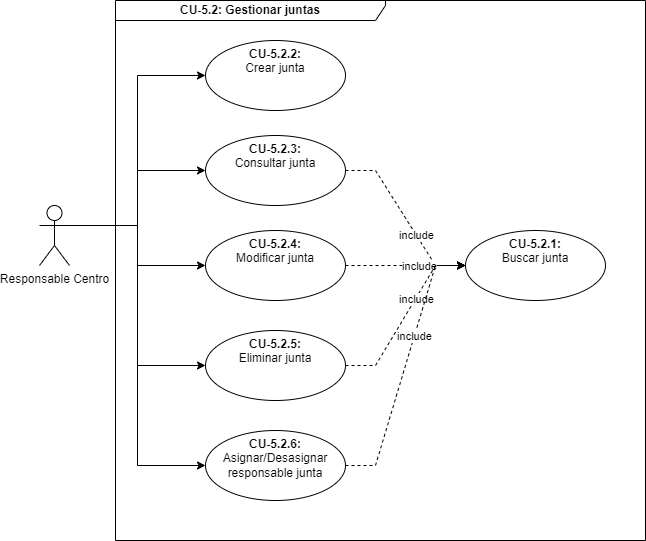
\includegraphics[scale=0.55]{img/diagramas/Funcional/CU-5.2.png}
        \caption{CU-5.2 Gestionar juntas}
        \label{fig:Diagrama-Caso de uso 5.2 Gestionar juntas}
    \end{figure}


\begin{table}[H]
    \caption{Gestionar miembros de gobierno}
    \label{tab:CU-5.3}
    \begin{center}
        \begin{tabular}{|l|p{12cm}|}
            \hline
            \multicolumn{2}{|c|}{Caso de uso 5.3 - Gestionar miembros de gobierno} \\
            \hline \hline
            Actores                 &   Responsable de centro          \\  
            \hline
            Descripción             &   Permite la gestión de los miembros de gobierno del centro responsable. \\  \hline
            Precondiciones          &   El usuario se debe haber identificado como responsable centro y elegido el caso de uso CU-5.3 Gestionar miembros de gobierno. \\  \hline
            Casos de uso            & 
            5.3.1 Buscar miembro de gobierno \\ 
            &
            5.3.2 Crear  miembro de gobierno \\ 
            & 
            5.3.3. Consultar miembro de gobierno\\ 
            & 
            5.3.4 Modificar miembro de gobierno \\ 
            &  
            5.3.5 Eliminar miembro de gobierno \\ 
            &
            5.3.6 Asignar/Desasignar responsable miembro de gobierno \\
            \hline
   
            Flujo principal         &   1. El sistema muestra la lista de los miembros de gobierno del centro responsable.   \\ 
            & 2a. Si no encuentra el miembro de gobierno que busca entonces puede crearlo. \\ 
            & 2b. Si encuentra el miembro de gobierno que busca entonces puede consultarlo, modificarlo o borrarlo. \\ \hline
            Flujo alternativo    &   1. Se produce un error al intentar ejecutar la opción elegida.  \\ 
            & 2. Se informa del error al usuario. \\
            & 3. El sistema vuelve a mostrar las opciones disponibles. \\
            \hline
        \end{tabular}
    \end{center}
\end{table}

\begin{figure}[H]
        \centering
        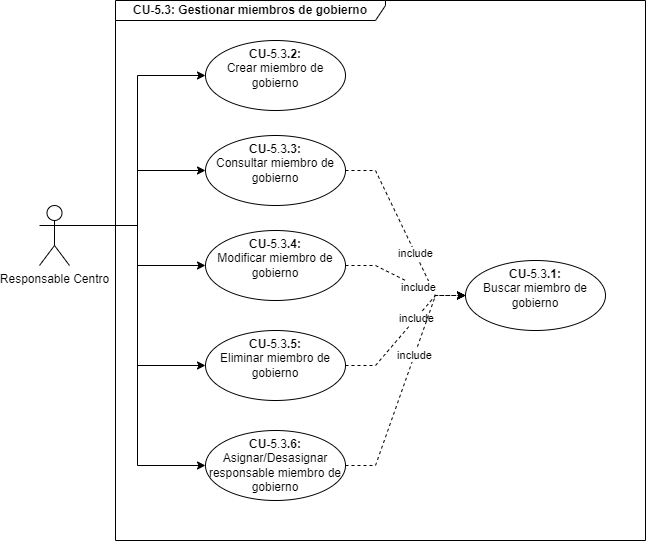
\includegraphics[scale=0.55]{img/diagramas/Funcional/CU-5.3.png}
        \caption{CU-5.3 Gestionar Gestionar miembros de gobierno}
        \label{fig:Diagrama-Caso de uso 5.3 Gestionar miembros de gobierno}
    \end{figure}


\begin{table}[H]
    \caption{Consultar ayuda de responsable centro}
    \label{tab:CU-5.4}
    \begin{center}
        \begin{tabular}{|l|p{12cm}|}
            \hline
            \multicolumn{2}{|c|}{Caso de uso 5.4 - Consultar ayuda de responsable centro} \\ \hline 
            Actores                 &   Responsable centro          \\  
            \hline
            Descripción        & Consultar ayuda de responsable centro    \\ \hline 
            Precondiciones          &   El usuario debe identificarse  como responsable centro y seleccionar el caso de uso CU-5.4 Consultar ayuda de responsable centro         \\  \hline
            Casos de uso            &          \\ \hline
            Flujo principal         &   1. El sistema muestra la información de ayuda 
            al usuario responsable centro.     \\\hline
            Flujo alternativo    &   1. Se produce un error al intentar mostrar la ayuda del usuario \\ 
            & 2. El sistema informa al usuario del error ocurrido. \\ 
            & 3. El sistema vuelve a mostrar al usuario las opciones disponibles (CU-5. Administrar centro).\\  \hline
        \end{tabular}
    \end{center}
\end{table}

\newpage


\subsection{CU-6. Administrar sistema}\label{sec:CU-6}    
El caso de uso \textit{CU-6. Administrar sistema  } describe las acciones que puede realizar el Usuario Administrador (véanse la Tabla \ref{tab:CU-6} y la Figura \ref{fig:Diagrama-Caso de uso 6. Administrar sistema}). Este caso de uso está compuesto por los siguientes sub-casos de uso que se describen en las tablas que se indican:
\begin{itemize}
  \item CU-6.1 Gestionar usuarios (Tabla \ref{tab:CU-6.1}).
  \item CU-6.2 Gestionar centros (Tabla \ref{tab:CU-6.2}).
  \item CU-6.3 Consultar la ayuda del administrador  (Tabla \ref{tab:CU-6.3}).
\end{itemize}

    \begin{table}[H]
        \caption{Administrar sistema}
        \label{tab:CU-6}
        \begin{center}
            \begin{tabular}{|l|p{10cm}|}
                \hline
                \multicolumn{2}{|c|}{Caso de uso 6 - Administrar sistema} \\ \hline \hline
                Actores                 &   Administrador        \\  \hline
                Descripción             &   Gestión del sistema. \\  \hline
                Precondiciones          &   El usuario se debe haber identificado como administrador y elegido el caso de uso CU-6. Administrar sistema           \\  \hline
                Casos de uso            
                & CU-6.1. Gestionar usuarios \\  
                & CU-6.2. Gestionar centros \\ 
                & CU-6.3. Consultar la ayuda del administrador \\
                \hline
                Flujo principal     & 1. El sistema muestra al administrador las opciones disponibles \\ 
                & 2. El administrador elige una de las opciones \\ 
                & 3. El sistema ejecuta la opción elegida. \\ 
                \hline
                Flujo alternativo    &   1. Error al ejecutar la opción elegida, \\ 
                & 2. Se informa al usuario del error ocurrido. \\ 
                & 3. El sistema vuelve a mostrar las opciones disponibles.  \\  
                \hline
            \end{tabular}
        \end{center}
    \end{table}
    
\begin{figure}[H]
        \centering
        \includegraphics[scale=0.55]{img/diagramas/Funcional/CU-6.png}
        \caption{CU-6. Administrar sistema}
        \label{fig:Diagrama-Caso de uso 6. Administrar sistema}
\end{figure}

\begin{table}[H]
    \caption{Gestionar usuarios}
    \label{tab:CU-6.1}
    \begin{center}
        \begin{tabular}{|l|p{12cm}|}
            \hline
            \multicolumn{2}{|c|}{Caso de uso 6.1 - Gestionar usuarios} \\ \hline \hline

            Actores                 &   Administrador\\  \hline
            Descripción             &   GEstionar información de un usuario universitario. \\  \hline
            Precondiciones          &   El usuario debe ser administrador  y escoger el caso de uso CU-6.1 Gestionar usuarios.        \\  \hline
            Casos de uso            & 6.1.1. Buscar usuario  \\ 
            & 6.1.2. Crear usuario \\ 
            & 6.1.3. Consultar usuario \\ 
            & 6.1.4. Modificar usuario \\ 
            & 6.1.5. Borrar usuario \\    
            \hline
            Flujo principal         &   1. El sistema muestra el listado de usuarios.   \\ 
            & 2a. Si no encuentra el usuario buscado, puede crearlo. \\ 
            & 2b. Si lo encuentra entonces lo puede consultar, modificar o eliminar.  \\ 
            \hline
            Flujo alternativo    &   1. Se produce un error al intentar mostrar la opción  elegida  \\ 
            & 2. El sistema informa al usuario del error. \\ 
            & 3. El sistema vuelve a mostrar al usuario las opciones disponibles.   \\  \hline
            
        \end{tabular}
    \end{center}
\end{table}

\begin{figure}[H]
        \centering
        \includegraphics[scale=0.55]{img/diagramas/Funcional/CU-6.1.png}
        \caption{CU-6.1 Gestionar usuarios}
        \label{fig:Diagrama-Caso de uso 6.1 Gestionar usuarios}
\end{figure}


\begin{table}[H]
    \caption{Gestionar centros}
    \label{tab:CU-6.2}
    \begin{center}
        \begin{tabular}{|l|p{12cm}|}
            \hline
            \multicolumn{2}{|c|}{Caso de uso 6.2 - Gestionar centros} \\ \hline \hline
            Actores                 &   Administrador\\  \hline
            Descripción             &   Permite la gestión de los centros universitarios. \\  \hline
            Precondiciones          &   El usuario debe ser administrador y escoger el caso de uso CU-6.2 Gestionar centros.          \\  \hline
            Casos de uso            & 6.2.1. Buscar centro  \\ 
            & 6.2.2. Crear centro \\ 
            & 6.2.3. Consultar centro \\ 
            & 6.2.4. Modificar centro \\ 
            & 6.2.5. Borrar centro \\ 
            \hline
            Flujo principal         &   1. El sistema muestra al administrador las opciones disponibles.   \\ 
            & 2. El administrador elige una de las opciones. \\ 
            & 3. El sistema ejecuta la opción elegida por el administrador. \\ 
            \hline
            Flujo alternativo    &   1. Se produce un error al ejecutar la opción elegida. \\ 
            & 2. Se informa al usuario del error ocurrido. \\ 
            & 3. El sistema vuelve a mostrar las opciones disponibles.  \\  
            \hline
        \end{tabular}
    \end{center}
\end{table}

\begin{figure}[H]
        \centering
        \includegraphics[scale=0.55]{img/diagramas/Funcional/CU-6.2.png}
        \caption{CU-6.2 Gestionar centros}
        \label{fig:Diagrama-Caso de uso 6.2 Gestionar centros}
\end{figure}


\begin{table}[H]
    \caption{Administrar sistema, consultar la ayuda del administrador}
    \label{tab:CU-6.3}
    \begin{center}
        \begin{tabular}{|l|p{12cm}|}
            \hline
            \multicolumn{2}{|c|}{Caso de uso 6.3 - Consultar la ayuda del administrador} \\ \hline \hline

            Actores                 &   Administrador   \\  \hline
            Descripción             &   Permite consultar la ayuda del administrador \\  \hline
            Precondiciones          &   El usuario debe ser administrador y escoger el caso de uso CU-6.3 Consultar la ayuda del administrador.         \\  \hline
            Casos de uso            &   
                                                   \\  \hline
            Flujo principal         &   1. El sistema mostrara la ayuda del administrador.        \\ \hline
            Flujo alternativo    &   1. Se produce un error al intentar mostrar la ayuda del usuario \\ & 2. El sistema informa al usuario del error. \\ & 3. El sistema vuelve a mostrar al usuario las opciones disponibles.   \\  \hline
            
        \end{tabular}
    \end{center}
\end{table}


\newpage

\section{Validación de casos de uso}
La tabla \ref{tab:Validación CU} permite comprobar que los casos de uso cubren todos los requisitos funcionales de la aplicación web propuestos en la Sección \ref{sec:requisitos-funcionales}.
\begin{table}[H]
    \centering
    \caption{Tabla validación casos de uso} \label{tab:Validación CU}
    \begin{tabular}{|l|l|}
        \hline
            \textbf{Requisito funcional} & \textbf{Caso de uso} \\ 
        \hline 
        \hline         
            \textbf{RF-1}  & CU 1.1 \\
            \textbf{RF-2}  & CU 1.2 \\ 
            \textbf{RF-3}  & CU 1.3 \\ 
            \textbf{RF-4}  & CU 1.3 \\ 
            \textbf{RF-5}  & CU 1.4 \\
            \textbf{RF-6}  & CU 1.4 \\ 
            \textbf{RF-7}  & CU 1.5 \\ 
        \hline
            \textbf{RF-8}  & CU 2.1 \\
            \textbf{RF-9}  & CU 2.2 \\
            \textbf{RF-10}  & CU 2.3 \\
        \hline
            \textbf{RF-11}  & CU 3.2 \\
            \textbf{RF-12}  & CU 3.3 \\
            \textbf{RF-13}  & CU 3.4 \\
        \hline
            \textbf{RF-14}  & CU 4.3 \\
            \textbf{RF-15}  & CU 4.2 \\
            \textbf{RF-17}  & CU 4.4 \\
            \textbf{RF-19}  & CU 4.5 \\
        \hline
            \textbf{RF-20}  & CU 5.3 \\
            \textbf{RF-21}  & CU 5.2 \\
            \textbf{RF-27}  & CU 5.4 \\
        \hline
            \textbf{RF-28}  & CU 6.2 \\
            \textbf{RF-36}  & CU 6.3 \\
            \textbf{RF-37}  & CU 6.1 \\

        \hline
    \end{tabular}%
    \end{table}
    
\newpage 

\section{Diagrama de secuencia}

%    El diagrama de secuencia es una representación gráfica que pretende dar una visión de las acciones que se realizarán durante la ejecución de alguna operación en el sistema. A continuación, se muestran los diagramas de secuencias para la creación (Figura  \ref{fig:Diagrama de secuencia crear comisión}), búsqueda (Figura \ref{fig:Diagrama de secuencia consultar comisión}), modificación (Figura \ref{fig:Diagrama de secuencia modificar comisión}) y borrado (Figura \ref{fig:Diagrama de secuencia borrar comisión}) de instancias genéricas (comisiones) que se corresponderán con los tipos de datos que se van a gestionar: centros, juntas, convocatorias, miembros de gobierno, miembros de junta, miembros de comisión, etc.

%\begin{figure}[H]
%        \centering
%        \includegraphics[scale=0.55]{img/diagramas/Secuencia/SEC-1.png}
%        \caption{Diagrama de secuencia de crear comisión}
%        \label{fig:Diagrama de secuencia crear comisión}
%    \end{figure}
    
    
%\begin{figure}[H]
%        \centering
%        \includegraphics[scale=0.55]{img/diagramas/Secuencia/SEC-2.png}
%        \caption{Diagrama de secuencia de consultar comisión}
%        \label{fig:Diagrama de secuencia buscar comisión}
%    \end{figure}
    
%\begin{figure}[H]
%        \centering
%        \includegraphics[scale=0.55]{img/diagramas/Secuencia/SEC-3.png}
%        \caption{Diagrama de secuencia de modificar comisión}
%        \label{fig:Diagrama de secuencia modificar comisión}
%\end{figure}
    
%\begin{figure}[H]
%        \centering
%        \includegraphics[scale=0.55]{img/diagramas/Secuencia/SEC-3.png}
%        \caption{Diagrama de secuencia de borrar comisión}
%        \label{fig:Diagrama de secuencia borrar comisión}
%    \end{figure}




\part{Diseño}
\chapter{Diseño de datos} \label{cap:diseño_datos}

\section{Introducción}
En este capítulo se definirán las estructuras de datos que conforman el sistema a partir de los elementos identificados durante el análisis de datos del Capítulo 7 (tipos de entidad y tipos de interrelación). Para ello, se llevarán a cabo los siguientes pasos:

\begin{itemize}
    \item Obtención del modelo relacional. Definición de la estructuras (tablas) del modelo de datos.
    \item Normalización del modelo. Refinamiento del modelo, para la eliminación de errores de integridad.
    \item Obtención del esquema relacional.
    \item Diagrama relacional.
\end{itemize}

 \section{Modelo Relacional}\label{sec:modelo-relacional}
A partir del Modelo Entidad - Interrelación descrito en el capítulo 7, se pueden obtener las tablas o relaciones del Modelo Relacional utilizando las reglas de transformación (RTECAR - véase el capítulo 5 de Bases de Datos. Desde Chen hasta Codd con ORACLE.\cite{reglasBD}). En concreto, se han aplicado las siguientes reglas de transformación:

\begin{itemize}
    \item RTECAR-1: Todos los tipos de entidad presentes en el esquema conceptual se transformarán en tablas o relaciones en el esquema relacional manteniendo el número y tipo de atributos, así como la característica de identificador de esos atributos.
    \item RTECAR-3.1: En las relaciones 1:N, la clave primaria de la entidad del lado 1 se convierte en una clave foránea en la tabla de la entidad del lado N.
\end{itemize}

Para cada tabla se mostrará la siguiente información:

\begin{itemize}
    \item \textbf{Descripción}. Se describirá el origen de la tabla, indicando los elementos del modelo Entidad-Interrelación desde los que se ha obtenido.
    \item \textbf{Nombre de la tabla}
    \item \textbf{Atributos}. Se describirán los atributos que componen la tabla, distinguiendo su rol en cada caso con la siguiente notación:
        \begin{itemize}
            \item Clave \underline{primaria}
            \item Clave ALTERNA, si existe
            \item Claves \textbf{foráneas}, si existen
            \item Resto de atributos
        \end{itemize}
    \item \textbf{Esquema relacional}. Definición formal de la tabla, de acuerdo con el Modelo Relacional.
\end{itemize}

\subsection{Tabla Tipo Centro}
    \begin{itemize}
        \item \textbf{Descripción}: la tabla Tipo Centro se obtiene a partir de la entidad \textit{Tipo Centro}.
        \item \textbf{Nombre de la tabla}: TipoCentro
        \item \textbf{Atributos}:
            \begin{itemize}
                \item Clave primaria: \underline{id}
                \item Clave alterna: ninguna.
                \item Clave foránea: ninguna.
                \item Resto de atributos: nombre, estado.
            \end{itemize}
        \item \textbf{Esquema relacional}: 
            TipoCentro (\textbf{\underline{id}}, nombre, estado)
    \end{itemize}

\subsection{Tabla Tipo Representación Gobierno}
    \begin{itemize}
        \item \textbf{Descripción}: la tabla Tipo Representación Gobierno se obtiene a partir de la entidad \textit{Tipo Representación Gobierno}.
        \item \textbf{Nombre de la tabla}: TipoRepresentaciónGobierno
        \item \textbf{Atributos}:
            \begin{itemize}
                \item Clave primaria: \underline{id}
                \item Clave alterna: ninguna
                \item Clave foránea: ninguna
                \item Resto de atributos: nombre, estado.
            \end{itemize}
        \item \textbf{Esquema relacional}: 
            TipoRepresentaciónGobierno(\textbf{\underline{id}}, nombre, estado)
    \end{itemize}

\subsection{Tabla Tipo Representación General}
    \begin{itemize}
        \item \textbf{Descripción}: la tabla Tipo Representación General se obtiene a partir de la entidad \textit{Tipo Representación General}.
        \item \textbf{Nombre de la tabla}: TipoRepresentaciónGeneral
        \item \textbf{Atributos}:
            \begin{itemize}
                \item Clave primaria: \underline{id}
                \item Clave alterna: ninguna
                \item Clave foránea: ninguna
                \item Resto de atributos: nombre, estado.
            \end{itemize}
        \item \textbf{Esquema relacional}: 
            TipoRepresentaciónGeneral(\textbf{\underline{id}}, nombre, estado)
    \end{itemize}

\subsection{Tabla Tipo Convocatoria}
    \begin{itemize}
        \item \textbf{Descripción}: la tabla Tipo Convocatoria se obtiene a partir de la entidad \textit{Tipo Convocatoria}.
        \item \textbf{Nombre de la tabla}: TipoRepresentaciónGeneral
        \item \textbf{Atributos}:
            \begin{itemize}
                \item Clave primaria: \underline{id}
                \item Clave alterna: ninguna
                \item Clave foránea: ninguna
                \item Resto de atributos: nombre, estado.
            \end{itemize}
        \item \textbf{Esquema relacional}: 
            TipoConvocatoria(\textbf{\underline{id}}, nombre, estado)
    \end{itemize}

\subsection{Tabla Usuario}
    \begin{itemize}
        \item \textbf{Descripción}: la tabla Usuario se obtiene a partir de la entidad \textit{Usuario}.
        \item \textbf{Nombre de la tabla}:
        \item \textbf{Atributos}:
            \begin{itemize}
                \item Clave primaria: \underline{id}
                \item Clave alterna: 
                \item Clave foránea: \textbf{}
                \item Resto de atributos: 
            \end{itemize}
        \item \textbf{Esquema relacional}: 
            Usuario(\textbf{\underline{id}}, name, email, password, estado)
    \end{itemize}

\subsection{Tabla Centro}
    \begin{itemize}
        \item \textbf{Descripción}: la tabla Centro se obtiene a partir de la entidad \textit{Centro}. Además, se incorpora la clave foránea \textbf{idTipo} de la tabla TipoCentro porque el tipo de entidad Centro presenta una debilidad por identificación respecto del tipo de entidad Tipo Centro.
        \item \textbf{Nombre de la tabla}: Centro
        \item \textbf{Atributos}:
            \begin{itemize}
                \item Clave primaria: \underline{id}
                \item Clave alterna: ninguna
                \item Clave foránea: \textbf{idTipo}
                \item Resto de atributos: nombre, dirección, estado
            \end{itemize}
        \item \textbf{Esquema relacional}: 
            Centro(\textbf{\underline{id}}, nombre, dirección, idTipo, estado)
    \end{itemize}

\subsection{Tabla Junta}
    \begin{itemize}
        \item \textbf{Descripción}: la tabla Junta se obtiene a partir de la entidad \textit{Junta}. Además, se incorpora la clave foránea \textbf{idCentro} de la tabla Centro porque el tipo de entidad Junta presenta una debilidad por identificación respecto del tipo de entidad Centro.
        \item \textbf{Nombre de la tabla}: Junta
        \item \textbf{Atributos}:
            \begin{itemize}
                \item Clave primaria: \underline{id}
                \item Clave alterna: ninguna
                \item Clave foránea: \textbf{idCentro}
                \item Resto de atributos: fechaConstitución, fechaDisolución, estado
            \end{itemize}
        \item \textbf{Esquema relacional}: 
            Junta(\textbf{\underline{id}}, fechaConstitución, fechaDisolución, idCentro, estado)
    \end{itemize}

\subsection{Tabla Comisión}
    \begin{itemize}
        \item \textbf{Descripción}: la tabla Comisión se obtiene a partir de la entidad \textit{Comisión}. Además, se incorpora la clave foránea \textbf{idJunta} de la tabla Junta porque el tipo de entidad Comisión presenta una debilidad por identificación respecto del tipo de entidad Junta.
        \item \textbf{Nombre de la tabla}: Comisión
        \item \textbf{Atributos}:
            \begin{itemize}
                \item Clave primaria: \underline{id}
                \item Clave alterna: ninguna
                \item Clave foránea: \textbf{idJunta}
                \item Resto de atributos: nombre, descripción, fechaConstitución, fechaDisolución, estado
            \end{itemize}
        \item \textbf{Esquema relacional}: 
            Comisión(\textbf{\underline{id}}, nombre, descripción, fechaConstitución, fechaDisolución, idJunta, estado)
    \end{itemize}

\subsection{Tabla Convocatoria}
    \begin{itemize}
        \item \textbf{Descripción}: la tabla Convocatoria se obtiene a partir de la entidad \textit{Convocatoria}. Además, se incorpora la clave foránea \textbf{idJunta} de la tabla Junta porque el tipo de entidad Convocatoria presenta una debilidad por identificación respecto del tipo de entidad Junta. Se incorpora la clave foránea \textbf{idComisión} de la tabla Comisión porque el tipo de entidad Convocatoria presenta una debilidad por identificación respecto del tipo de entidad Comisión. Se incorpora la clave foránea \textbf{idTipo} de la tabla TipoConvocatoria porque el tipo de entidad Convocatoria presenta una debilidad por identificación respecto del tipo de entidad TipoConvocatoria.
        \item \textbf{Nombre de la tabla}: Convocatoria
        \item \textbf{Atributos}:
            \begin{itemize}
                \item Clave primaria: \underline{id}
                \item Clave alterna: ninguna
                \item Clave foránea: \textbf{idJun}, \textbf{idCom}, \textbf{idTipo}
                \item Resto de atributos: lugar, fecha, hora, estado
            \end{itemize}
        \item \textbf{Esquema relacional}: 
            Convocatoria(\textbf{\underline{id}}, lugar, fecha, hora, idTipo, idJun, idCom, estado)
    \end{itemize}

\subsection{Tabla Miembro Gobierno}
    \begin{itemize}
        \item \textbf{Descripción}: la tabla MiembroGobierno se obtiene a partir de la entidad \textit{Miembro Gobierno}. Además, se incorpora la clave foránea \textbf{idUsuario} de la tabla Junta porque el tipo de entidad MiembroGobierno presenta una debilidad por identificación respecto del tipo de entidad Usuario. Se incorpora la clave foránea \textbf{idCentro} de la tabla Centro porque el tipo de entidad MiembroGobierno presenta una debilidad por identificación respecto del tipo de entidad Centro. Se incorpora la clave foránea \textbf{idRepresentación} de la tabla TipoRepresentaciónGobierno porque el tipo de entidad MiembroGobierno presenta una debilidad por identificación respecto del tipo de entidad TipoRepresentaciónGobierno.
        \item \textbf{Nombre de la tabla}: MiembroGobierno
        \item \textbf{Atributos}:
            \begin{itemize}
                \item Clave primaria: \underline{id}
                \item Clave alterna: ninguna
                \item Clave foránea: \textbf{idUsuario}, \textbf{idCentro}, \textbf{idRepresentación}
                \item Resto de atributos: fechaTomaPosesión, fechaCese, estado
            \end{itemize}
        \item \textbf{Esquema relacional}: 
            MiembroGobierno(\textbf{\underline{id}}, fechaTomaPosesión, fechaCese, idUsuario, idCentro, idRepresentación, estado)
    \end{itemize}

\subsection{Tabla Miembro Junta}
    \begin{itemize}
        \item \textbf{Descripción}: la tabla MiembroJunta se obtiene a partir de la entidad \textit{Miembro Junta}. Además, se incorpora la clave foránea \textbf{idUsuario} de la tabla Junta porque el tipo de entidad MiembroJunta presenta una debilidad por identificación respecto del tipo de entidad Usuario. Se incorpora la clave foránea \textbf{idJunta} de la tabla Centro porque el tipo de entidad MiembroJunta presenta una debilidad por identificación respecto del tipo de entidad Junta. Se incorpora la clave foránea \textbf{idRepresentación} de la tabla TipoRepresentaciónGeneral porque el tipo de entidad MiembroJunta presenta una debilidad por identificación respecto del tipo de entidad TipoRepresentaciónGeneral.
        \item \textbf{Nombre de la tabla}: MiembroGobierno
        \item \textbf{Atributos}:
            \begin{itemize}
                \item Clave primaria: \underline{id}
                \item Clave alterna: ninguna
                \item Clave foránea: \textbf{idUsuario}, \textbf{idJunta}, \textbf{idRepresentación}
                \item Resto de atributos: fechaTomaPosesión, fechaCese, estado
            \end{itemize}
        \item \textbf{Esquema relacional}: 
            MiembroJunta(\textbf{\underline{id}}, fechaTomaPosesión, fechaCese, idUsuario, idJunta, idRepresentación, estado)
    \end{itemize}

\subsection{Tabla Miembro Comisión}
    \begin{itemize}
        \item \textbf{Descripción}: la tabla MiembroComisión se obtiene a partir de la entidad \textit{Miembro Comisión}. Además, se incorpora la clave foránea \textbf{idUsuario} de la tabla Junta porque el tipo de entidad MiembroComisión presenta una debilidad por identificación respecto del tipo de entidad Usuario. Se incorpora la clave foránea \textbf{idComisión} de la tabla Centro porque el tipo de entidad MiembroJunta presenta una debilidad por identificación respecto del tipo de entidad Comisión. Se incorpora la clave foránea \textbf{idRepresentación} de la tabla TipoRepresentaciónGeneral porque el tipo de entidad MiembroJunta presenta una debilidad por identificación respecto del tipo de entidad TipoRepresentaciónGeneral.
        \item \textbf{Nombre de la tabla}: MiembroComisión
        \item \textbf{Atributos}:
            \begin{itemize}
                \item Clave primaria: \underline{id}
                \item Clave alterna: ninguna
                \item Clave foránea: \textbf{idUsuario}, \textbf{idComisión}, \textbf{idRepresentación}
                \item Resto de atributos: fechaTomaPosesión, fechaCese, estado
            \end{itemize}
        \item \textbf{Esquema relacional}: 
            MiembroComisión(\textbf{\underline{id}}, fechaTomaPosesión, fechaCese, idUsuario, idComisión, idRepresentación, estado)
    \end{itemize}
    
 \section{Normalización del modelo}\label{sec:normalizacion}
La normalización del modelo descrito en la sección anterior pretende detectar y corregir redundancias e inconsistencias en la información representada, para lo cual se aplicarán las medidas correctoras que garanticen que las tablas obtenidas cumplen las siguientes formas normalizadas \cite{reglasBD}.

\begin{itemize}
    \item Primera Forma Normal (FN1): una relación R satisface la FN1 si y solo si, todos los dominios subyacentes de la relación R (atributos) contienen valores atómicos.
    \item Segunda Forma Normal (FN2): una relación R satisface la FN2 si y sólo si, satisface la FN1 y cada atributo de la relación depende funcionalmente de forma completa de la clave primaria de esa relación.
    \item Tercera Forma Normal (FN3): una relación R satisface la FN3 si y sólo si, satisface la FN2 y cada atributo no primo de la relación no depende funcionalmente de forma transitiva de la clave primaria de esa relación, es decir, no pueden existir dependencias transitivas entre los atributos que no forman parte de la clave primaria de esa relación R.
    \item Forma Normal de Boyce-Codd (FNBC): una relación R satisface la FNBC si y sólo si, se encuentra en FN1 y cada determinante funcional es una clave candidata de la relación R, denominándose determinante funcional a uno o un conjunto de atributos de una relación R del cual depende funcionalmente de forma completa algún otro atributo de la misma relación.
\end{itemize}

Todas las tablas definidas se encuentran en la Primera Forma Normal, puesto que en ninguna de ellas existen atributos múltiples.

\subsection{Tabla TipoCentro}
    \begin{itemize}
        \item \textbf{Claves candidatas}: id
        \item \textbf{Normalización}: La tabla TipoCentro presenta una dependencia funcional formada por la clave primaria y el resto de atributos. La tabla se encuentra en FNBC: el único determinante funcional es la clave primaria, por lo que la dependencia funcional con el resto de atributos es completa.
    \end{itemize}

\begin{figure}[H]
\centering
\includegraphics[scale=0.75]{img/diagramas/Datos/FNBC-TipoCentro.png}
\caption{Tabla TipoCentro en FNBC}\label{fig:Tabla TipoCentro en FNBC}   
\end{figure}

\subsection{Tabla TipoRepresentaciónGobierno}
    \begin{itemize}
        \item \textbf{Claves candidatas}: id
        \item \textbf{Normalización}: La tabla TipoRepresentaciónGobierno presenta una dependencia funcional formada por la clave primaria y el resto de atributos. La tabla se encuentra en FNBC: el único determinante funcional es la clave primaria, por lo que la dependencia funcional con el resto de atributos es completa.
    \end{itemize}

\begin{figure}[H]
\centering
\includegraphics[scale=0.75]{img/diagramas/Datos/FNBC-TipoRepresentaciónGobierno.png}
\caption{Tabla TipoRepresentaciónGobierno en FNBC}\label{fig:Tabla TipoRepresentaciónGobierno en FNBC}   
\end{figure}

\subsection{Tabla TipoRepresentaciónGeneral}
    \begin{itemize}
        \item \textbf{Claves candidatas}: id
        \item \textbf{Normalización}: La tabla TipoRepresentaciónGeneral presenta una dependencia funcional formada por la clave primaria y el resto de atributos. La tabla se encuentra en FNBC: el único determinante funcional es la clave primaria, por lo que la dependencia funcional con el resto de atributos es completa.
    \end{itemize}

\begin{figure}[H]
\centering
\includegraphics[scale=0.75]{img/diagramas/Datos/FNBC-TipoRepresentaciónGeneral.png}
\caption{Tabla TipoRepresentaciónGeneral en FNBC}\label{fig:Tabla TipoRepresentaciónGeneral en FNBC}   
\end{figure}

\subsection{Tabla TipoConvocatoria}
    \begin{itemize}
        \item \textbf{Claves candidatas}: id
        \item \textbf{Normalización}: La tabla TipoConvocatoria presenta una dependencia funcional formada por la clave primaria y el resto de atributos. La tabla se encuentra en FNBC: el único determinante funcional es la clave primaria, por lo que la dependencia funcional con el resto de atributos es completa.
    \end{itemize}

\begin{figure}[H]
\centering
\includegraphics[scale=0.75]{img/diagramas/Datos/FNBC-TipoConvocatoria.png}
\caption{Tabla TipoConvocatoria en FNBC}\label{fig:Tabla TipoConvocatoria en FNBC}   
\end{figure}

\subsection{Tabla Usuario}
    \begin{itemize}
        \item \textbf{Claves candidatas}: id
        \item \textbf{Normalización}: La tabla Usuario presenta una dependencia funcional formada por la clave primaria y el resto de atributos. La tabla se encuentra en FNBC: el único determinante funcional es la clave primaria, por lo que la dependencia funcional con el resto de atributos es completa.
    \end{itemize}

\begin{figure}[H]
\centering
\includegraphics[scale=0.75]{img/diagramas/Datos/FNBC-Usuario.png}
\caption{Tabla Usuario en FNBC}\label{fig:Tabla Usuario en FNBC}   
\end{figure}

\subsection{Tabla Centro}
    \begin{itemize}
        \item \textbf{Claves candidatas}: id
        \item \textbf{Normalización}: La tabla Centro presenta una dependencia funcional formada por la clave primaria y el resto de atributos. La tabla se encuentra en FNBC: el único determinante funcional es la clave primaria, por lo que la dependencia funcional con el resto de atributos es completa.
    \end{itemize}

\begin{figure}[H]
\centering
\includegraphics[scale=0.75]{img/diagramas/Datos/FNBC-Centro.png}
\caption{Tabla Centro en FNBC}\label{fig:Tabla Centro en FNBC}   
\end{figure}

\subsection{Tabla Junta}
    \begin{itemize}
        \item \textbf{Claves candidatas}: id
        \item \textbf{Normalización}: La tabla Junta presenta una dependencia funcional formada por la clave primaria y el resto de atributos. La tabla se encuentra en FNBC: el único determinante funcional es la clave primaria, por lo que la dependencia funcional con el resto de atributos es completa.
    \end{itemize}

\begin{figure}[H]
\centering
\includegraphics[scale=0.75]{img/diagramas/Datos/FNBC-Junta.png}
\caption{Tabla Junta en FNBC}\label{fig:Tabla Junta en FNBC}   
\end{figure}

\subsection{Tabla Comisión}
    \begin{itemize}
        \item \textbf{Claves candidatas}: id
        \item \textbf{Normalización}: La tabla Comisión presenta una dependencia funcional formada por la clave primaria y el resto de atributos. La tabla se encuentra en FNBC: el único determinante funcional es la clave primaria, por lo que la dependencia funcional con el resto de atributos es completa.
    \end{itemize}

\begin{figure}[H]
\centering
\includegraphics[scale=0.75]{img/diagramas/Datos/FNBC-Comisión.png}
\caption{Tabla Comisión en FNBC}\label{fig:Tabla Comisión en FNBC}   
\end{figure}

\subsection{Tabla Convocatoria}
    \begin{itemize}
        \item \textbf{Claves candidatas}: id
        \item \textbf{Normalización}: La tabla Convocatoria presenta una dependencia funcional formada por la clave primaria y el resto de atributos. La tabla se encuentra en FNBC: el único determinante funcional es la clave primaria, por lo que la dependencia funcional con el resto de atributos es completa.
    \end{itemize}

\begin{figure}[H]
\centering
\includegraphics[scale=0.75]{img/diagramas/Datos/FNBC-Convocatoria.png}
\caption{Tabla Convocatoria en FNBC}\label{fig:Tabla Convocatoria en FNBC}   
\end{figure}

\subsection{Tabla MiembroGobierno}
    \begin{itemize}
        \item \textbf{Claves candidatas}: id
        \item \textbf{Normalización}: La tabla MiembroGobierno presenta una dependencia funcional formada por la clave primaria y el resto de atributos. La tabla se encuentra en FNBC: el único determinante funcional es la clave primaria, por lo que la dependencia funcional con el resto de atributos es completa.
    \end{itemize}

\begin{figure}[H]
\centering
\includegraphics[scale=0.75]{img/diagramas/Datos/FNBC-MiembroGobierno.png}
\caption{Tabla MiembroGobierno en FNBC}\label{fig:Tabla MiembroGobierno en FNBC}   
\end{figure}

\subsection{Tabla MiembroJunta}
    \begin{itemize}
        \item \textbf{Claves candidatas}: id
        \item \textbf{Normalización}: La tabla MiembroJunta presenta una dependencia funcional formada por la clave primaria y el resto de atributos. La tabla se encuentra en FNBC: el único determinante funcional es la clave primaria, por lo que la dependencia funcional con el resto de atributos es completa.
    \end{itemize}

\begin{figure}[H]
\centering
\includegraphics[scale=0.75]{img/diagramas/Datos/FNBC-MiembroJunta.png}
\caption{Tabla MiembroJunta en FNBC}\label{fig:Tabla MiembroJunta en FNBC}   
\end{figure}

\subsection{Tabla MiembroComisión}
    \begin{itemize}
        \item \textbf{Claves candidatas}: id
        \item \textbf{Normalización}: La tabla MiembroComisión presenta una dependencia funcional formada por la clave primaria y el resto de atributos. La tabla se encuentra en FNBC: el único determinante funcional es la clave primaria, por lo que la dependencia funcional con el resto de atributos es completa.
    \end{itemize}

\begin{figure}[H]
\centering
\includegraphics[scale=0.75]{img/diagramas/Datos/FNBC-MiembroComisión.png}
\caption{Tabla MiembroComisión en FNBC}\label{fig:Tabla MiembroComisión en FNBC}   
\end{figure}

 \section{Esquema relacional}\label{sec:esquema-relacional}

\begin{table}[H]
\begin{center}
    \begin{tabular}{|l|p{8cm}|}
    \hline
    Tabla                 &   Atributos          
    \\ \hline
    TipoCentro             &   (\textbf{\underline{id}}, nombre, estado) 
    \\  \hline
    TipoRepresentaciónGobierno          &   (\textbf{\underline{id}}, nombre, estado)
    \\  \hline
    TipoRepresentaciónGeneral             &   (\textbf{\underline{id}}, nombre, estado) 
    \\  \hline
    TipoConvocatoria             &   (\textbf{\underline{id}}, nombre, estado) 
    \\  \hline
    Usuario             &   (\textbf{\underline{id}}, name, email, password, estado) 
    \\  \hline
    Centro             &   (\textbf{\underline{id}}, nombre, dirección, idTipo, estado) 
    \\  \hline
    Junta             &   (\textbf{\underline{id}}, fechaConstitución, fechaDisolución, idCentro, estado) 
    \\  \hline
    Comisión             &    (\textbf{\underline{id}}, nombre, descripción, fechaConstitución, fechaDisolución, idJunta, estado) 
    \\  \hline
    Convocatoria             &    (\textbf{\underline{id}}, lugar, fecha, hora, idTipo, idJun, idCom, estado)
    \\  \hline
    MiembroGobierno             &   (\textbf{\underline{id}}, fechaTomaPosesión, fechaCese, idUsuario, idCentro, idRepresentación, estado) 
    \\  \hline
    MiembroJunta             &   (\textbf{\underline{id}}, fechaTomaPosesión, fechaCese, idUsuario, idJunta, idRepresentación, estado)
    \\  \hline
    MiembroComisión             &   (\textbf{\underline{id}}, fechaTomaPosesión, fechaCese, idUsuario, idComisión, idRepresentación, estado)
    \\  \hline
            \end{tabular}
        \end{center}
    \end{table}



\section{Diagrama relacional}\label{sec:diagrama-relacional}
El diagrama relacional del modelo propuesto se muestra en la figura \ref{fig:Diagrama Relacional}.

\begin{landscape}
\begin{figure}[H]
\centering
\includegraphics[scale=0.3]{img/diagramas/Datos/Diagrama-relacional.png}
\caption{Diagrama relacional}\label{fig:Diagrama Relacional}   
\end{figure}
\end{landscape}




\chapter{Diseño arquitectónico} \label{cap:arquitectura}

\section{Introducción}

\section{Diagrama de despliegue}

\subsection{Descripción de los nodos}

\subsection{Descripción de los componentes}
\chapter{Diseño de la interfaz} \label{cap:diseño_interfaz}

\section{Introducción}

\section{Características comunes}

\section{Interfaz del módulo Usuario Público}
\subsection{Descripción general}
ghjk
\subsection{Descripción detallada}
ghjk
\subsection{Otros elementos de la interfaz}
hjk

\section{Interfaz del módulo Usuario Registrado}
\subsection{Descripción general}
hjk
\subsection{Descripción detallada}
hjk
\subsection{Otros elementos de la interfaz}
hjk

\section{Interfaz del módulo Representante Comisión}
\subsection{Descripción general}
hjk
\subsection{Descripción detallada}
hjk
\subsection{Otros elementos de la interfaz}
hjk

\section{Interfaz del módulo Representante Junta}
\subsection{Descripción general}
hjk
\subsection{Descripción detallada}
hjk
\subsection{Otros elementos de la interfaz}
hjk

\section{Interfaz del módulo Representante Centro}
\subsection{Descripción general}
hjk
\subsection{Descripción detallada}
hjk
\subsection{Otros elementos de la interfaz}
hjk

\section{Interfaz del módulo Administrador}
\subsection{Descripción general}
hjk
\subsection{Descripción detallada}
hjk
\subsection{Otros elementos de la interfaz}
hjk








\part{Pruebas}
\chapter{Pruebas}\label{cap:pruebas}

\section{Introducción}

\section{Prueba de usuarios públicos}

\subsection{Pruebas CU-1.1}
 \begin{itemize}
    \item Prueba realizada
    \item Resultado de la prueba
    \item Prueba realizada
    \item Resultado de la prueba
 \end{itemize}

\section{Prueba de usuarios universitarios registrados}

\subsection{Pruebas CU-1.1}
 \begin{itemize}
    \item Prueba realizada
    \item Resultado de la prueba
    \item Prueba realizada
    \item Resultado de la prueba
 \end{itemize}

\section{Prueba de módulo responsable comisión}
\subsection{Pruebas CU-1.1}
 \begin{itemize}
    \item Prueba realizada
    \item Resultado de la prueba
    \item Prueba realizada
    \item Resultado de la prueba
 \end{itemize}

 \section{Prueba de módulo responsable junta}
\subsection{Pruebas CU-1.1}
 \begin{itemize}
    \item Prueba realizada
    \item Resultado de la prueba
    \item Prueba realizada
    \item Resultado de la prueba
 \end{itemize}

  \section{Prueba de módulo responsable centro}
\subsection{Pruebas CU-1.1}
 \begin{itemize}
    \item Prueba realizada
    \item Resultado de la prueba
    \item Prueba realizada
    \item Resultado de la prueba
 \end{itemize}

  \section{Prueba de módulo administrador}
\subsection{Pruebas CU-1.1}
 \begin{itemize}
    \item Prueba realizada
    \item Resultado de la prueba
    \item Prueba realizada
    \item Resultado de la prueba
 \end{itemize}



\part{Conclusiones y futuras mejoras}
\chapter{Conclusiones}

\section{Introducción}
En este capítulo se exponen la conclusiones obtenidas sobre el desarrollo del proyecto, y en relación con los objetivos planteados inicialmente en el capítulo 2 frente al resultado final alcanzado tras la finalización del mismo y las pruebas realizadas. 

Con carácter general, el objetivo principal, consistente en el desarrollo de un sistema informático integrado para la gestión de comisiones de la Universidad de Córdoba, se ha cumplido satisfactoriamente, logrando una solución que anteriormente no existía.

\section{Conclusiones específicas}

\section{Conclusiones personales y profesionales}
A nivel personal, el presente trabajo me ha permitido reciclar, actualizar y adquirir nuevos conocimientos técnicos, especialmente en el uso de Frameworks como Laravel. Estos Frameworks facilitan el desarrollo de software escalable y eficiente, lo que permitirá abordar nuevas funcionalidades de manera segura en el futuro.

En cuanto al ámbito profesional, se han logrado los objetivos propuestos:

\begin{itemize}

\item La Universidad de Córdoba dispone ahora de una herramienta personalizada para el desarrollo de su trabajo, que ha demostrado, a lo largo de todo el periodo de pruebas, cubrir suficientemente las necesidades planteadas, sin perjuicio de las mejoras que se proponen en el capítulo 14.

\item La experiencia acumulada durante el desarrollo de este trabajo permite asentar conocimientos sobre el desarrollo de aplicaciones web, así como la utilización de las tecnologías que están a la orden del día, permitiendo con ello un constante aprendizaje continuo en esta materia. 

\end{itemize}



\chapter{Futuras mejoras}

\section{Introducción}
El sistema desarrollado en este trabajo es susceptible de mejoras y ampliaciones, como cualquier otro software. De hecho, se identificaron muchas oportunidades durante el desarrollo.

Las mejoras contempladas se pueden agrupar en diferentes vertientes según su propósito o naturaleza:

\begin{itemize}
    \item Mejoras y nuevas funciones. Esta categoría incluye cambios que hacen que el software sea más eficiente, fácil de usar o funcional.
    
    \item Integración con otras aplicaciones. El desarrollo de nuevas aplicaciones en la Sección de Soporte u otros entornos similares puede dar lugar a la implementación de conectividades entre todos los sistemas. Esto contribuiría a una mayor eficiencia en el desarrollo del trabajo.
    
    \item Capacidad de extensión y exportación. Además, es importante considerar la posibilidad de exportar este sistema a otras unidades organizativas de la universidad o de otras organizaciones.
\end{itemize}

En todo caso, el hecho de que se aborden las mejoras aquí propuestas, en su totalidad o en parte, dependerá, en última instancia, de la continuidad de su uso, puesto que, tal como se indicó en la sección 3.4, el sistema desarrollado tendrá un uso provisional.

En las siguientes secciones se desglosan las mejoras y ampliaciones propuestas, según cada una de las categoría expuestas.

\section{Mejoras y nuevas funciones}
Basándonos en lo que se ha desarrollado hasta ahora, se identifican una serie de funciones adicionales y mejoras que se pueden realizar. Estas mejoras se describen a continuación, divididas por tipo de usuario y mejoras generales.

\subsection{Mejoras para usuarios}
\begin{itemize}
    \item Generar más tipos de certificados, con más información detallada
    \item COn respecto al usuario público, poder consultar información en un periodo de tiempo de las comisiones de la Universidad de Córdoba, en lugar de solamente las actuales.
\end{itemize}

\subsection{Mejoras para responsables}
\begin{itemize}
    \item Añadir más opciones de trámites automatizados (correos a terceros, por ejemplo).
    \item Permitir el tratamiento masivo de miembros. Por ejemplo, crear a la vez los miembros de junta de una junta en concreto, siendo la fecha de toma de posesión la misma, ya que normalmente al crearse una junta la toma de posesión de la mayoría de los miembros es el mismo día.
\end{itemize}

\subsection{Mejoras para administradores}
\begin{itemize}
    \item Añadir más opciones de filtros por cada tipo de entidad para una mayor precisión de localización del elemento a buscar.
    \item Generar estadísticas sobre el uso de la aplicación.
    \item Añadir funcionalidad de supervisión de las acciones realizadas por diferentes roles, como por ejemplo, consultar porcentaje de absentismo de asistencia a las convocatorias de comisión y junta.
\end{itemize}

\subsection{Mejoras de funcionamiento}
\begin{itemize}
    \item Hacer más eficiente el proceso de gestión de las paradas de tramitación y el cálculo de los tiempos de tramitación.
    \item Establecer y registrar los motivos por los que un trabajo se cierra o termina, para facilitar la comprensión y el seguimiento del trabajo realizado.
    \item Permitir que los usuarios puedan personalizar la aplicación, ya que su uso podría extenderse en el tiempo y algunos apartados podrían cambiar.
\end{itemize}

\subsection{Integración con otras aplicaciones}
Se propone integrar la aplicación con otras aplicaciones que se utilizan actualmente o que puedan utilizarse en el futuro por el personal de la Universidad de Córdoba.

Se pudo observar en una visita al Rectorado de Córdoba, como se utilizaban múltiples aplicaciones web separadas por funcionalidad, teniendo cada una de ellas un acceso diferente, duplicado y poco conectado entre ellas.

Una gran mejora sería la de unificar todas ellas en un sistema en conjunto como si de la Intranet de la Universidad de Córdoba se tratara. Actualmente se pudo observar como el personal laboral tenía en el navegador web en una lista de favoritos enlaces a cada una de las aplicaciones web desarrolladas para la gestión de cada tarea.

\subsection{Exportabilidad}
Para que la aplicación pueda exportarse a otros entornos, se deben definir como variables de entorno los elementos que dependen de la ubicación o configuración específica del entorno deseado.

\begin{itemize}
    \item Conectores y cuentas sociadas
    \item Ubicación y denominación de orígenes de datos
\end{itemize}


\addcontentsline{toc}{chapter}{Bibliografía}

%\bibliographystyle{vancouver}
%\printbibheading[heading=bibintoc]
\printbibliography
\renewcommand{\appendixpagename}{Anexos}
\renewcommand{\appendixtocname}{Anexos}
\renewcommand{\appendixname}{Anexo}

\end{document}